\chapter{Representative numerical simulations -- II}
\label{numerical-simulations-2}

The theoretical framework developed in the preceding chapter resulted
in a set of coupled partial differential equations governing the
interrelated mechanics, mass transport and biochemistry pertinent to
biological tissue growth. In order to demonstrate the applicability of
the theory, this chapter presents the results of several illustrative
numerical experiments posed within a corresponding computational
framework retaining all aspects of the coupling between the equations.

The chapter begins by providing some insight into the numerical
methods used to solve the coupled equations in Section~\ref{eu%
  -computational-model}. The first set of examples, presented in
Section~\ref{simple-physics}, serve to illustrate basic aspects of the
coupled physics underlying biphasic models for tissue mechanics. In
Section~\ref{biphasic-examples-2}, the biphasic model parameters are
tailored to be more representative of experimental studies on the
mechanics of engineered ligaments, and aspects of the time- and
rate-dependent behaviour of the model are explored. The final example
presented in this chapter provides a straightforward extension of the
theory to model the effects of the mechanical environment on growing
tumours (Section~\ref{tumour-growth}), evidencing the generality of
the proposed formulation.

\section{Introducing the computational model}
\label{eu-computational-model}

The mathematical formulation developed in Chapter~\ref{eulerian%
  -perspective} has been implemented in a finite element setting using
{\tt COMSOL Multiphysics},\footnote{\href {http://www.comsol.com/}
  {http://www.comsol.com/}} a computational environment for solving
coupled systems of partial differential equations. For simplicity, the
numerical implementation is in two spatial dimensions assuming a state
of plain strain, and it uses triangular elements of order 2 (quadratic
elements) to approximate the displacement field of the solid phase,
and triangular elements of order 1 (linear elements) to approximate
all other field variables, including the fluid velocity and
concentration. A representative unstructured mesh, used in the
computations on a unit square domain in Section~\ref{simple-physics},
is shown in Figure~\ref{egmesh2d} and consists of 3267 elements.

\begin{figure}[ht]
  \centering
  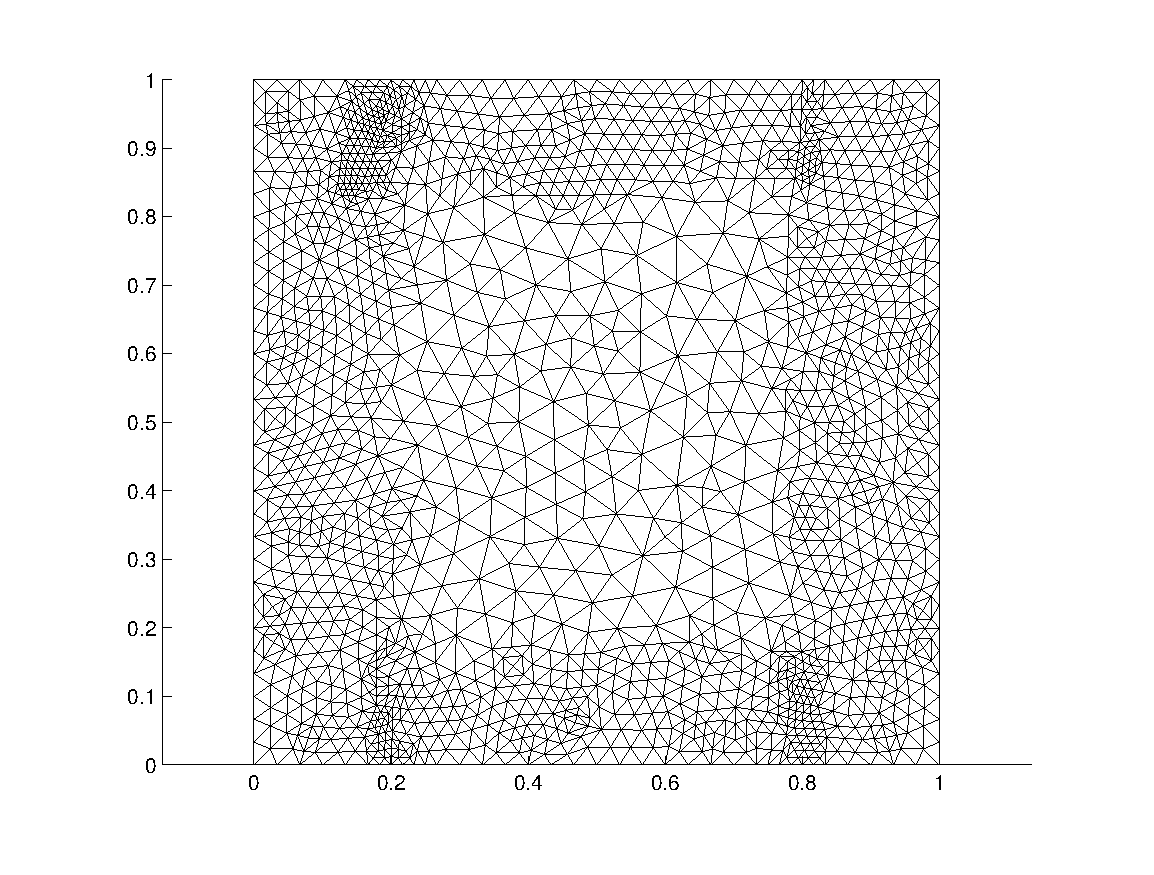
\includegraphics[width=0.8\textwidth]{images/examples/%
    eulerian/mesh}
  \caption{A representative unstructured finite element mesh used in
    the computations.}
  \label{egmesh2d}
\end{figure}

In the numerical implementation presented in Chapter~\ref{numerical%
  -simulations-1}, a simplified form of the balance of momentum was
imposed by treating the tissue as a whole and solving a summation of
Equation~(\ref{localbalanceofmomentum}) over all species. This
simplification necessitated additional assumptions on the underlying
micro-mechanics, and these were discussed in
Section~\ref{constriction-1}. In contrast, the implementation used in
this chapter solves the {\em detailed} momentum balance equations;
enforcing the balance of momentum for each species separately. The
coupling between the mechanics equations of the individual species is
introduced by specifying momentum transfer terms, $\bq^{\iota}$,
arising from frictional interaction as discussed in
Section~\ref{eu-interaction-forces}.

The balance of mass~(\ref{localbalanceofmass}) and
momentum~(\ref{localbalanceofmomentum}) equations for the solid
collagen are solved in the reference configuration of the tissue,
$\Omega_{0}$, and the balance of mass~(\ref{eu-localbalanceofmass})
and momentum~(\ref{eu-localbalanceofmomentum}) equations for the fluid
phase are solved in the current configuration, $\Omega_{t}$. Recall
that this choice is justified because we know the reference
configuration of the solid phase of the tissue. These equations, along
with the saturation constraint discussed below, are solved
simultaneously for the for the solid
concentration,~$\rho_{0}^{\mathrm{c}}$, and
displacement,~$\bu^{\mathrm{c}}$; and the fluid
concentration,~$\rho^{\mathrm{f}}$, velocity,~$\bv^{\mathrm{f}}$, and
pressure,~$p^{\mathrm{f}}$. Variable-order backward difference
formulae \citep{leveque2007} are used for forwarding the equations
through time.

In the interest of generality, the formulation and corresponding
implementation presented in Chapters~\ref{lagrangian-perspective} and
\ref{numerical-simulations-1} allowed for the possibility of
cavitation in tissues under certain ex~vivo/in~vitro
conditions. However, since it is well established that under normal
physiological conditions soft tissues are fully saturated by the
fluid, this condition will be imposed in the following calculations.

The concentration of each species~$\iota$ can be expressed as the
product of two non-negative scalar fields: $\rho^\iota = \phi^\iota
\tilde{\rho}^\iota$, where $\phi^\iota$ is the volume fraction and
$\tilde{\rho}^\iota$ is the intrinsic density of species~$\iota$ in
$\Omega_{t}$. The mixture is said to be saturated if the total volume
fraction, \mbox{$\phi = \sum\limits_{\iota}\phi^\iota = 1$}
\citep{passmanetal}. Since the solute species are present only in very
low concentrations, the preceding condition can be suitably
approximated by:\footnote{The saturation condition, as stated in
  Equation (\ref{eu-saturationconstraint}), incorporates an implicit
  assumption that the solid and fluid phases of the tissue are
  individually {\em intrinsically} incompressible. This means that
  their intrinsic densities, $\tilde{\rho}^\iota$, do not change under
  load, and this is a common assumption employed in the soft tissue
  mechanics literature. (See, for e.g., \citet{mowetal1980} and
  \citet{ateshian07}.)}

\begin{equation}
\frac{\left(\rho_{0}^{\mathrm{c}}/J\right)}
     {\tilde{\rho}^{\mathrm{c}}} +
     \frac{\rho^{\mathrm{f}}}{\tilde{\rho}^{\mathrm{f}}} = 1.
\label{eu-saturationconstraint}
\end{equation}

\noindent In this computational implementation, the fluid
pressure,~$p^{\mathrm{f}}$, is not constitutively specified in terms
of the current concentration of the fluid, and instead serves as an
indeterminate Lagrange multiplier to impose the saturation
constraint~(\ref{eu-saturationconstraint}).

For simplicity, in the calculations that follow, the strain energy
function used for the elastic portion of the response of the solid
collagen is the model of Mooney and Rivlin \citep{mooney1940}:

\begin{equation}
\hat{\psi^{\mathrm{c}}} (\bC^{\mathrm{e}}) = \sum\limits_{i,j=0}^{n}
C_{ij} (I_{1}-3)^{i} (I_{2}-3)^{j}
\label{mooney-rivlin-model}
\end{equation}

\noindent (where $I_{1}$ and $I_{2}$ are the first and second
principal invariants of the elastic right Cauchy-Greent tensor,
$\bC^{\mathrm{e}}$), suitably decomposed into volumetric and isochoric
parts. A mixed displacement-pressure \citep{ZienkTay:89} formulation
is used to treat the near-incompressibility of the solid phase. Also
for simplicity, the fluid is assumed to be ideal, i.e. the fluid
viscosity, $\mu^{\mathrm{f}}=0$~Pa.s.

\section{Some simple physical tests}
\label{simple-physics}

The preliminary calculations presented in this section aim to
illustrate basic aspects of the coupled physics that arise in mixture
models that include only two non-reacting phases: a solid and a
fluid. In these calculations, the tissue is assumed to be $1$~mm thick
and the material model for the solid phase uses the Mooney-Rivlin
strain energy function~(\ref{mooney-rivlin-model}) with just one term
having the material constant \mbox{$C_{10} = 0.8$~MPa.}

\subsection{An inflating balloon}
\label{balloon}

This example studies the inflation of the tissue as a result of
pressure-gradient driven influx of fluid.  The total duration of the
test is 3~s. The initial concentrations of the solid collagen and
fluid phases at all points in a unit square domain \mbox{(1~mm
  $\times$ 1~mm)} are 500~kg.m$^{-3}$, and their intrinsic densities
are 1000~kg.m$^{-3}$. Thus, each phase has an initial volume fraction
of 0.5. At the initial time, the solid displacement and velocity
fields, and the fluid velocity and pressure fields are each 0 in their
respective units at all points in the domain.

The boundary conditions for this problem correspond to holding the
bottom edge of the tissue fixed to prevent rigid body motion, and
forcing inflow of the fluid at this bottom edge while disallowing
outflow at any of the other edges, simulating an inflating balloon. In
particular:

\begin{itemize}
\item For the fluid, the boundary condition on the bottom edge
  specifies that its pressure increases linearly in time from 0~MPa to
  0.3~MPa during the duration of this test. The boundary condition for
  the fluid on the other three edges specifies that its velocity field
  is the same as that of the solid, $\bv^{\mathrm{f}} =
  \bv^{\mathrm{c}}$, disallowing outflow of fluid.
\item For the solid, the boundary condition on the bottom edge fixes
  the components of the solid displacement to 0~mm for the entire
  duration of the test. On the other three edges, following literature
  on fluid-structure interaction \citep{doneaetal2004}, there is a
  traction boundary condition on the solid that reads,
  $\bt^{\mathrm{c}}=\Bsigma^{\mathrm{c}} \bn = -p^{\mathrm{f}} \bn$,
  suitably pulled-back to the reference configuration. Here, $\bn$ is
  the normal to $\Omega_{t}$, and this condition relates the stress in
  the solid to the pressure in the fluid along the edges where there
  is no relative motion between the solid and the fluid.\footnote{In
    contrast to the swelling example discussed in
    Section~\ref{swelling-1}, which used the notion of the growth
    portion of the deformation gradient of the fluid,
    $\bF^{\mathrm{g}^\mathrm{f}}$, to cause kinematic swelling of the
    domain with an increase in fluid concentration, in this example,
    it is primarily this interaction between the solid and fluid
    stresses on the boundary that causes the domain to swell.}
\end{itemize}

In this example, the frictional coefficient tensor, $\bD^{\mathrm{fc}}
= 1\mathrm{e}^{-5} \ \bone$~MPa.s.mm$^{-2}$, is assumed to have a
relatively small magnitude because we are currently more interested in
observing the swelling of the domain due to fluid influx rather than
the frictional interaction between the phases.

Figures~\ref{swelling-balloon-image-0p0}--\ref{swelling-balloon%
  -image-3p0} show snapshots of the swelling domain during the course
of the test. The colour contours provide the horizontal displacement
field of the solid (in~mm) and the arrows provide the direction of the
solid velocity field. The pressure gradient induced by the increasing
fluid pressure boundary condition on the bottom edge causes an inflow
of fluid. The inability of the fluid to flow out of other boundaries
manifests itself as an outward boundary traction on the solid, causing
the domain to swell as seen in the figures.  Because the computation
was run with dynamics, there is initially a small oscillation in the
fluid and solid velocity fields due to wave propagation in the fluid
(not apparent in the plots) which fade in the first 0.4~s.

\begin{figure}[!hptb]
  \centering
  \includegraphics[width=0.9\textwidth]{images/examples/%
    eulerian/swelling/balloon-swell-0p0}
  \caption{The inflating balloon at time $t=0$ s.} 
  \label{swelling-balloon-image-0p0}
\end{figure}

\begin{figure}[!hptb]
  \centering
  \includegraphics[width=0.9\textwidth]{images/examples/%
    eulerian/swelling/balloon-swell-0p6}
  \caption{The inflating balloon at time $t=0.6$ s.} 
  \label{swelling-balloon-image-0p6}
\end{figure}

\begin{figure}[!hptb]
  \centering
  \includegraphics[width=0.9\textwidth]{images/examples/%
    eulerian/swelling/balloon-swell-1p2}
  \caption{The inflating balloon at time $t=1.2$ s.} 
  \label{swelling-balloon-image-1p2}
\end{figure}

\begin{figure}[!hptb]
  \centering
  \includegraphics[width=0.9\textwidth]{images/examples/%
    eulerian/swelling/balloon-swell-1p8}
  \caption{The inflating balloon at time $t=1.8$ s.} 
  \label{swelling-balloon-image-1p8}
\end{figure}

\begin{figure}[!hptb]
  \centering
  \includegraphics[width=0.9\textwidth]{images/examples/%
    eulerian/swelling/balloon-swell-2p4}
  \caption{The inflating balloon at time $t=2.4$ s.} 
  \label{swelling-balloon-image-2p4}
\end{figure}

\begin{figure}[!hptb]
  \centering
  \includegraphics[width=0.9\textwidth]{images/examples/%
    eulerian/swelling/balloon-swell-3p0}
  \caption{The inflating balloon at time $t=3.0$ s.} 
  \label{swelling-balloon-image-3p0}
\end{figure}

\clearpage

\subsection{The tissue under constriction}
\label{constriction-2}

In the previous numerical experiment, we studied the deformation of
the tissue under an influx of fluid. In this example, we turn our
attention to fluid flow fields induced by the deformation of the solid
phase and frictional interactions between the phases. The initial
condition for this problem is identical to the previous case, i.e.,
the tissue is at rest initially and the initial concentrations of the
solid collagen and fluid phases at all points in the unit square
domain \mbox{(1~mm $\times$ 1~mm)} are 500~kg.m$^{-3}$. As before, the
total duration of the test is 3~s.

\begin{figure}[!hptb]
  \centering
  \psfrag{u}{$u$ (mm)}
  \psfrag{y}{$y$ (mm)}
  \psfrag{t}{$t$ (s)}
  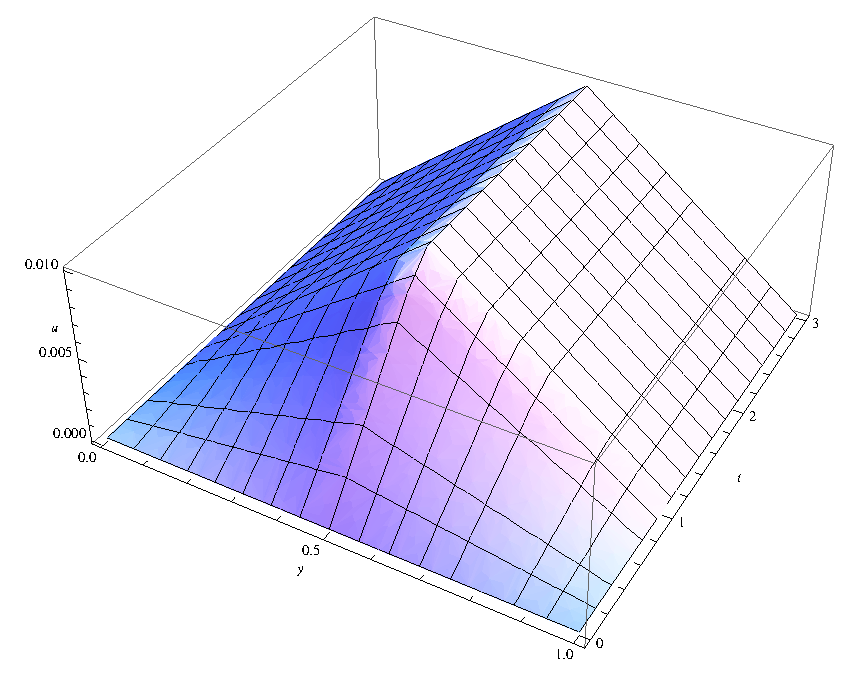
\includegraphics[width=0.8\textwidth]{images/examples/%
    eulerian/constriction/displacement-load}
  \caption{The magnitude of the displacement load on the vertical
    edges of the tissue.}
  \label{eu-constrict-disp-load}
\end{figure}

The boundary conditions for this problem correspond to immersing the
tissue in a bath and applying a displacement load on the vertical
edges so as to constrict the tissue in order to observe the resulting
fluid flow. In particular, the fluid is subjected to a pressure
boundary condition on all four edges; where the pressure of the fluid
is equated to that of the bath,~0~MPa. For the solid, the bottom edge
is held fixed and the top edge is traction free. The left edge is
subjected to the temporally-varying constrictive horizontal
displacement (in~mm) visualised in Figure~\ref{eu-constrict%
  -disp-load}. The figure shows the horizontal displacement being
increased linearly in time for the first 1~s and then held fixed for
the remainder of the test. The right edge is subjected to the negative
of this load. In this example, the magnitude of the frictional
coefficient tensor, $\bD^{\mathrm{fc}} = \bone$~MPa.s.mm$^{-2}$, is
significantly greater than in the previous case, and the effects of
the frictional interaction between the phases are manifest in the
results.

Figures~\ref{constrict-image-0p0}--\ref{constrict-image-3p0} show
snapshots of the constricted tissue during the course of the test. The
colour contours provide the horizontal displacement field of the solid
(in~mm) which remains fixed after the first 1~s of the test. The
arrows provide the direction and magnitude of the fluid velocity
field. Their lengths scale linearly with the magnitude of the fluid
velocity field and the longest arrow corresponds to a fluid velocity
magnitude of 7.03e-3 mm.s$^{-1}$. This fluid flow is mainly driven by
a combination of frictional interaction with the solid phase and the
saturation condition. The plots are asymmetrical in the vertical
direction because the bottom edge is held fixed. Observe that the
fluid velocity grows with increasing constriction of the solid for the
first 1~s and gradually decays after the solid phase is held fixed
(this is clearly seen in seen in Figure~\ref{velocity-evolution%
  -dynamic}). There is also a nominal relaxation of the top edge after
the constriction phase, as observed in the example in Section~\ref%
{constriction-1}.

As in the previous example, effects from the dynamics were observed in
this case as well, and an equivalent quasistatic calculation was
performed for comparison. When the vertical fluid velocity is tracked
at the centre of the top edge for the duration of the test in both
these cases, it is observed that the dynamic case decays gradually and
has oscillations (Figure~\ref{velocity-evolution-dynamic}) while the
quasistatic case reaches a higher magnitude, and decays nearly
instantaneously without manifesting oscillations
(Figure~\ref{velocity-evolution-quasistatic}).

\begin{figure}[!hptb]
  \centering
  \includegraphics[width=0.9\textwidth]{images/examples/%
    eulerian/constriction/constrict-0p0}
  \caption{The constricted tissue at time $t=0$ s.} 
  \label{constrict-image-0p0}
\end{figure}

\begin{figure}[!hptb]
  \centering
  \includegraphics[width=0.9\textwidth]{images/examples/%
    eulerian/constriction/constrict-0p32}
  \caption{The constricted tissue at time $t=0.32$ s.} 
  \label{constrict-image-0p32}
\end{figure}

\begin{figure}[!hptb]
  \centering
  \includegraphics[width=0.9\textwidth]{images/examples/%
    eulerian/constriction/constrict-0p66}
  \caption{The constricted tissue at time $t=0.66$ s.} 
  \label{constrict-image-0p66}
\end{figure}

\begin{figure}[!hptb]
  \centering
  \includegraphics[width=0.9\textwidth]{images/examples/%
    eulerian/constriction/constrict-1p0}
  \caption{The constricted tissue at time $t=1.0$ s.} 
  \label{constrict-image-1p0}
\end{figure}

\begin{figure}[!hptb]
  \centering
  \includegraphics[width=0.9\textwidth]{images/examples/%
    eulerian/constriction/constrict-2p0}
  \caption{The constricted tissue at time $t=2.0$ s.} 
  \label{constrict-image-2p0}
\end{figure}

\begin{figure}[!hptb]
  \centering
  \includegraphics[width=0.9\textwidth]{images/examples/%
    eulerian/constriction/constrict-3p0}
  \caption{The constricted tissue at time $t=3.0$ s.} 
  \label{constrict-image-3p0}
\end{figure}

\begin{figure}[!hptb]
  \centering
  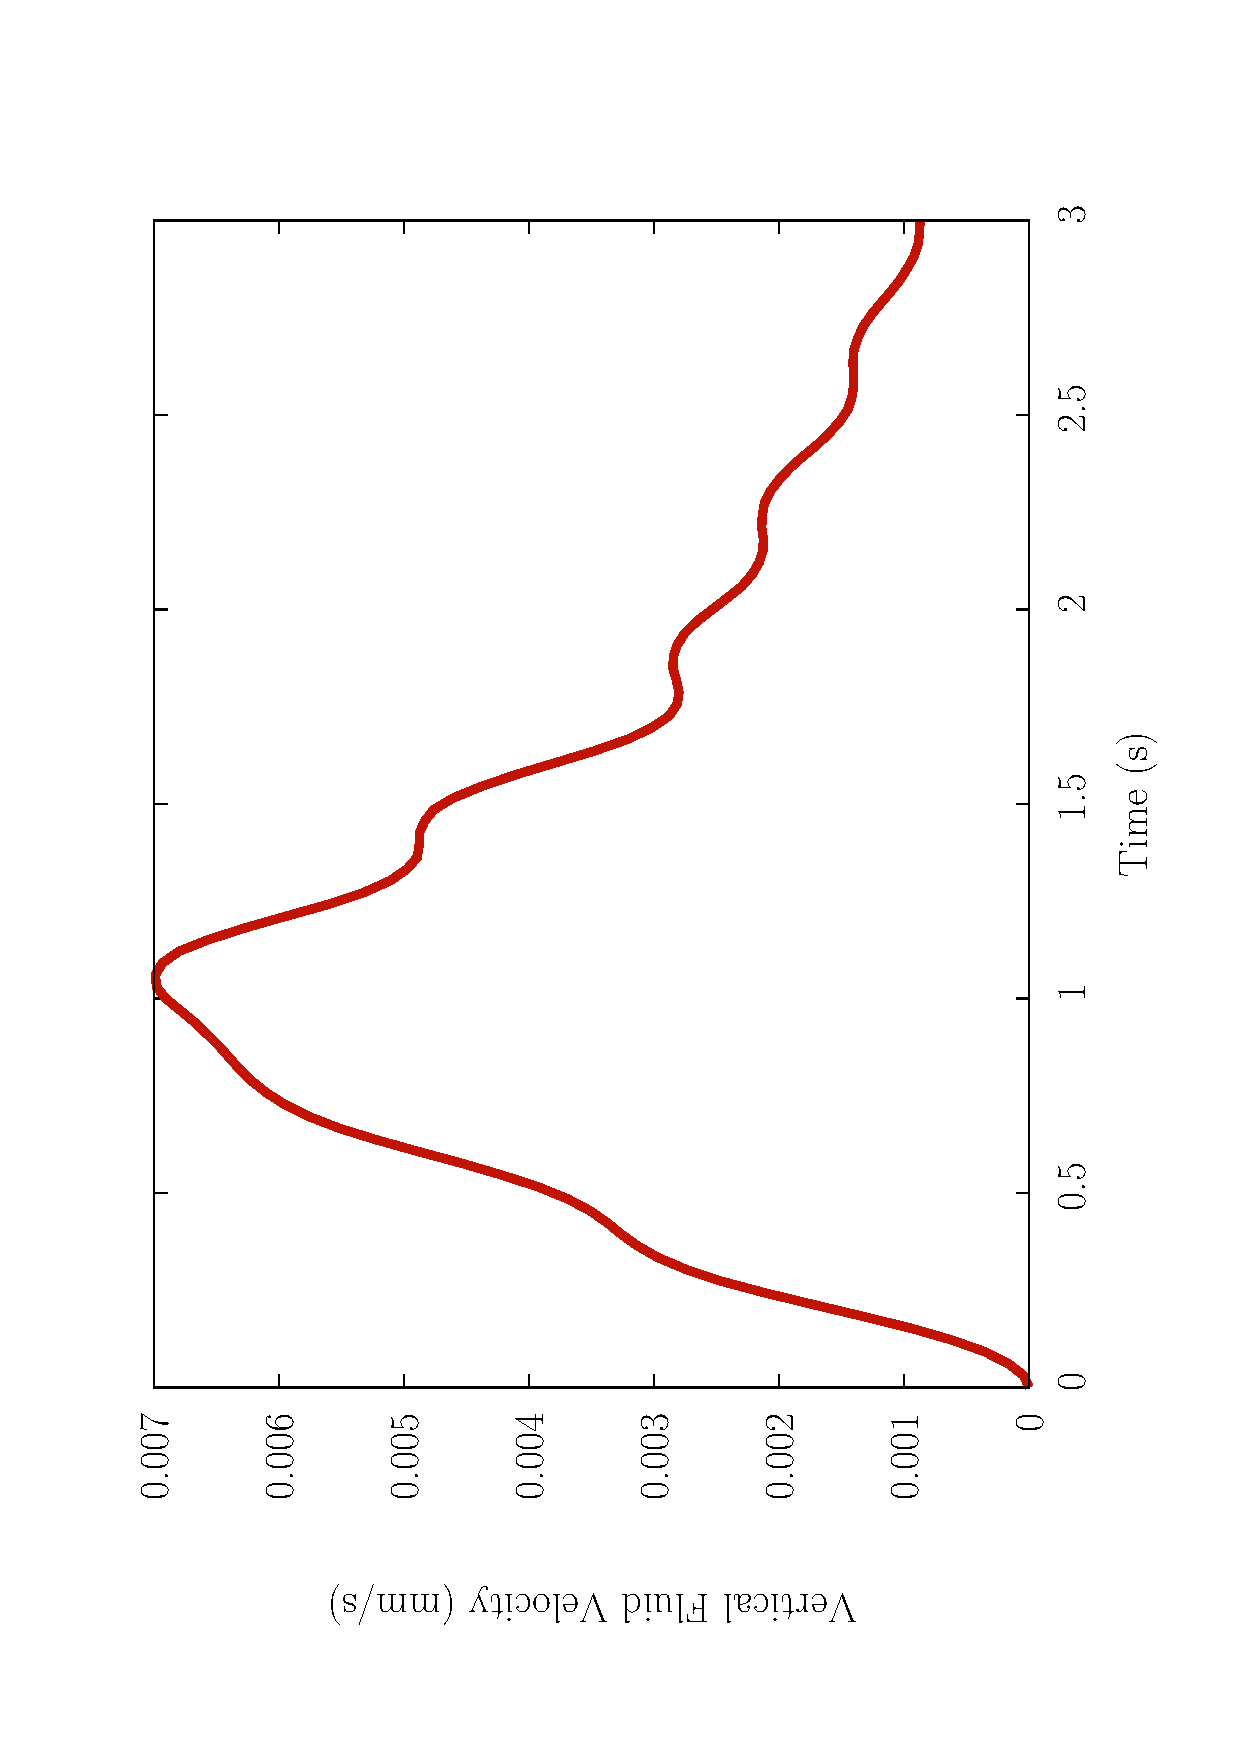
\includegraphics[width=0.6\textwidth,angle=270]{images/examples/%
    eulerian/constriction/constrict-vel-drop-dynamic}
  \caption{Dynamic evolution of the vertical fluid velocity.}
  \label{velocity-evolution-dynamic}
\end{figure}

\begin{figure}[!hptb]
  \centering
  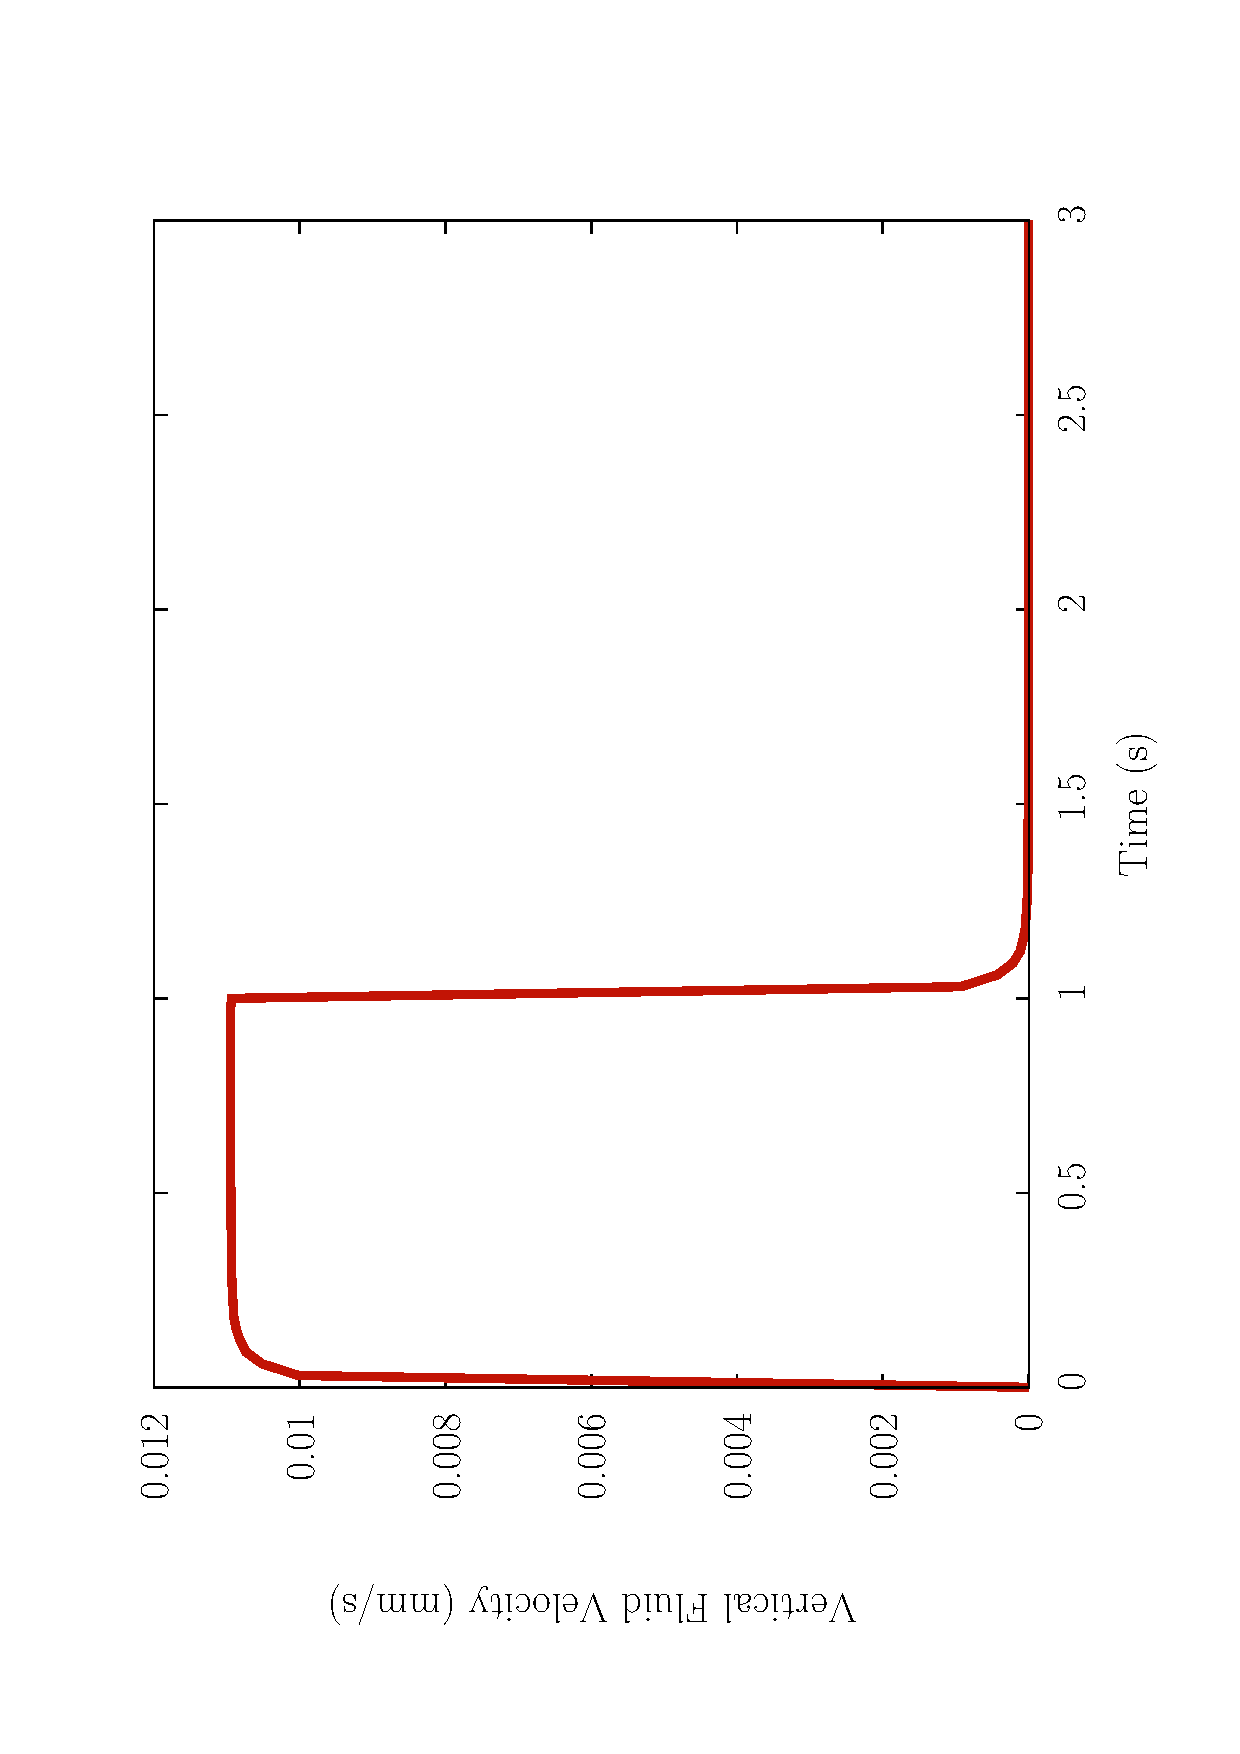
\includegraphics[width=0.6\textwidth,angle=270]{images/examples/%
    eulerian/constriction/constrict-vel-drop-quasistatic}
  \caption{Quasistatic evolution of the vertical fluid velocity.}
  \label{velocity-evolution-quasistatic}
\end{figure}

\clearpage

\section{Examples exploring the biphasic nature of porous soft
  tissues}
\label{biphasic-examples-2}

The introductory examples presented in the preceding section
illustrated basic aspects of the coupled physics exhibited by
non-reacting two-phase mixtures. The computational formulation thus
provides a means for determining the evolution of fluid flow fields
under varying physically-relevant boundary conditions, and allows us
to study their effects on the mechanics of tissues. With this
established, we now turn our attention to a more realistic
application---studying aspects of the time- and rate-dependent
behaviour of ligaments.

In the following examples, the material parameters and model geometry
are tailored to more closely represent experimental studies on the
mechanics of engineered ligaments \citep{Syed-Picard:06}. The examples
focus on the viscoelastic behaviour of these tissues arising primarily
from frictional interaction between two purely elastic phases: an
ideal fluid perfusing a porous, hyperelastic solid (as in the
preceding section). In particular cases, this {\em poroelastic}
response is compared to analogous results obtained using a
single-phase linear viscoelastic solid model (discussed in
Section~\ref{eu-viscoelastic-solid}).

Motivated by the experimental work, the model geometry is initially
12~mm in length and 1.128~mm in width, and has a uniform thickness of
1.128~mm. The initial concentration of the solid collagen is
300~kg.m$^{-3}$ and the initial fluid concentration is 700~kg.m$^{-3}$
at all points in the domain. The intrinsic densities of the solid
collagen and fluid phases are both 1000~kg.m$^{-3}$, as before. The
hyperelastic model for the solid phase uses the Mooney-Rivlin strain
energy function~(\ref{mooney-rivlin-model}) with 9 terms, and the
values of the corresponding parameters used in the analysis are
reported in Table~\ref{parameters-explant}.

\begin{table}[!hptb]
  \centering
  \begin{tabular}{|c|c|}
    \hline Parameter & Value (GPa) \\
    \hline \hline
    $C_{10}$  &   0$\phantom{.00000}$  \\
    $C_{01}$  &   0$\phantom{.00000}$  \\
    $C_{20}$  &   0.54434  \\
    $C_{11}$  &   0$\phantom{.00000}$  \\
    $C_{02}$  &   0.54714  \\
    $C_{30}$  &   1.83688  \\
    $C_{21}$  &   1.19985  \\
    $C_{12}$  &   10.6863  \\
    $C_{03}$  &   38.3875  \\
    \hline
  \end{tabular}
  \caption{Material constants corresponding to the explanted
    ligament (Figure~\ref{explanted-ligament}).}
  \label{parameters-explant}
\end{table}

The initial solid and fluid concentrations, and the Mooney-Rivlin
parameters chosen, approximate the collagen content and the tensile
response of the explanted ligament\footnote{This tissue is from a
  batch of engineered ligaments explanted after implantation for one
  month as medial collateral ligament replacements in live rats
  \citep{Syed-Picard:06}.} whose mechanical response under repeated
cyclic loading is shown in Figure~\ref{explanted-ligament}. In
particular, the hyperelastic material parameters are chosen to
approximate the stress-strain response corresponding to the first load
excursion (denoted by the blue points).

\begin{figure}[!hptb]
  \centering
  \includegraphics[width=0.8\textwidth]{images/experiments/%
    explant-cyclic-load}
  \caption{Mechanical response of an explanted ligament
    \citep{Syed-Picard:06}.}
  \label{explanted-ligament}
\end{figure}

The basal magnitude of the frictional coefficient tensor used in
following calculations is fit to the experimental work of
\citet{Swartzetal:99} on fluid transport through mouse tails. This was
achieved by subjecting the computational model to a fluid pressure
gradient identical to that in their experiment, and the frictional
coefficient tensor magnitude was modified until the until the
steady-state flow velocity in the computations matched those reported
in the experiment. The resulting frictional coefficient tensor is:
$\bD^{\mathrm{fc}} = 1.037 \ \bone$~MPa.s.mm$^{-2}$. In what follows,
this isotropic tensor will be characterised by its scalar magnitude,
$D$.

\subsection{Stress relaxation}
\label{stress-relaxation}

In these tests, the boundary conditions correspond to gripping the
tissue at its longitudinal ends, and loading the tissue at a constant
strain rate to a specific strain and holding it fixed at that strain
for the remainder of the test. For the solid phase, this translates to
holding one of the longitudinal edges fixed while subjecting the other
to the suitable displacement load. The lateral edges of the solid
remain traction free. For the fluid, there is no flow relative to the
solid at the longitudinal edges, i.e., $\bv^{\mathrm{f}} =
\bv^{\mathrm{c}}$. Since we are simulating the tissue being held by
grips at the longitudinal edges, this boundary condition ensures that
there is no outflow or inflow along those edges. The lateral edges
expose the fluid to the bath, and therefore the fluid pressure is
equated to that of the bath, 0~MPa, along those edges.

Figure~\ref{poro-stress-relax-0p01} shows the stress relaxation in a
quasistatic calculation\footnote{Since the displacement condition
  applied to the solid is not smooth in time, the corresponding
  velocity boundary condition on the fluid is discontinuous in
  time. Consequently, the poroelastic calculations presented in this
  section assume that the process is quasistatic; only requiring that
  the velocity fields be integrable in time.}  where the tissue is
loaded at a strain rate of $\dot{\epsilon}=0.01$ Hz to a maximum
strain of 0.085 in 8.5~s, and then held fixed at that strain for the
remainder of the test. A large portion of the tensile response is
furnished by the hyperelastic solid collagen, and the decaying peak in
the stress is due to the decaying relative velocity between the two
phases. Notice that this peak in stress decays rapidly, corresponding
to the rapidly decaying velocity field in the quasistatic result shown
in Figure~\ref{velocity-evolution-quasistatic}.

In order to study the effects of the load rate on the mechanical
response, the next test doubles the strain rate to $\dot{\epsilon} =
0.02$ Hz. The tissue is subjected to the same maximum strain of 0.085,
now in 4.25~s, and is held fixed for the remainder of the test. The
stress relaxation resulting from this test is shown in
Figure~\ref{poro-stress-relax-0p02}. The initial peak stress is now
increased; an observation which is in agreement with classical results
in viscoelasticity theory. This is because the increased strain rate
results in an increased relative velocity between the phases
initially, which correspondingly increases the frictional interaction
between the phases.

Finally, the biphasic poroelastic response is compared to the response
of a model comprising of only one phase: linear viscoelastic solid
collagen. In this computation, the elastic portion of the response of
the solid collagen has the same form~(\ref{mooney-rivlin-model}) and
material properties (Table~\ref{parameters-explant}) as the
poroelastic case, and has a characteristic relaxation time,
$\tau=0.3$~s, and strain-energy factor, $\beta=0.5$.\footnote{Refer
  Section~\ref{eu-viscoelastic-solid} for details.} This test is
carried out at a strain rate of $\dot{\epsilon}=0.02$~Hz for 4.25~s,
at which point the tissue is held fixed. Figure~\ref{visco-stress%
  -relax-0p02-t0p3} shows the corresponding stress relaxation, and
there are two noticeable differences in the results from the
poroelastic calculation performed at the same strain rate
(Figure~\ref{poro-stress-relax-0p02}).  Firstly, stemming from the
initially high relative velocity between the phases, the poroelastic
curve starts with a higher stiffness than the viscoelastic case. And
secondly, the quasistatic nature of the poroelastic calculation
results in a sharper, more rapidly-decaying peak in stress.

\clearpage

\begin{figure}[!hptb]
  \centering
  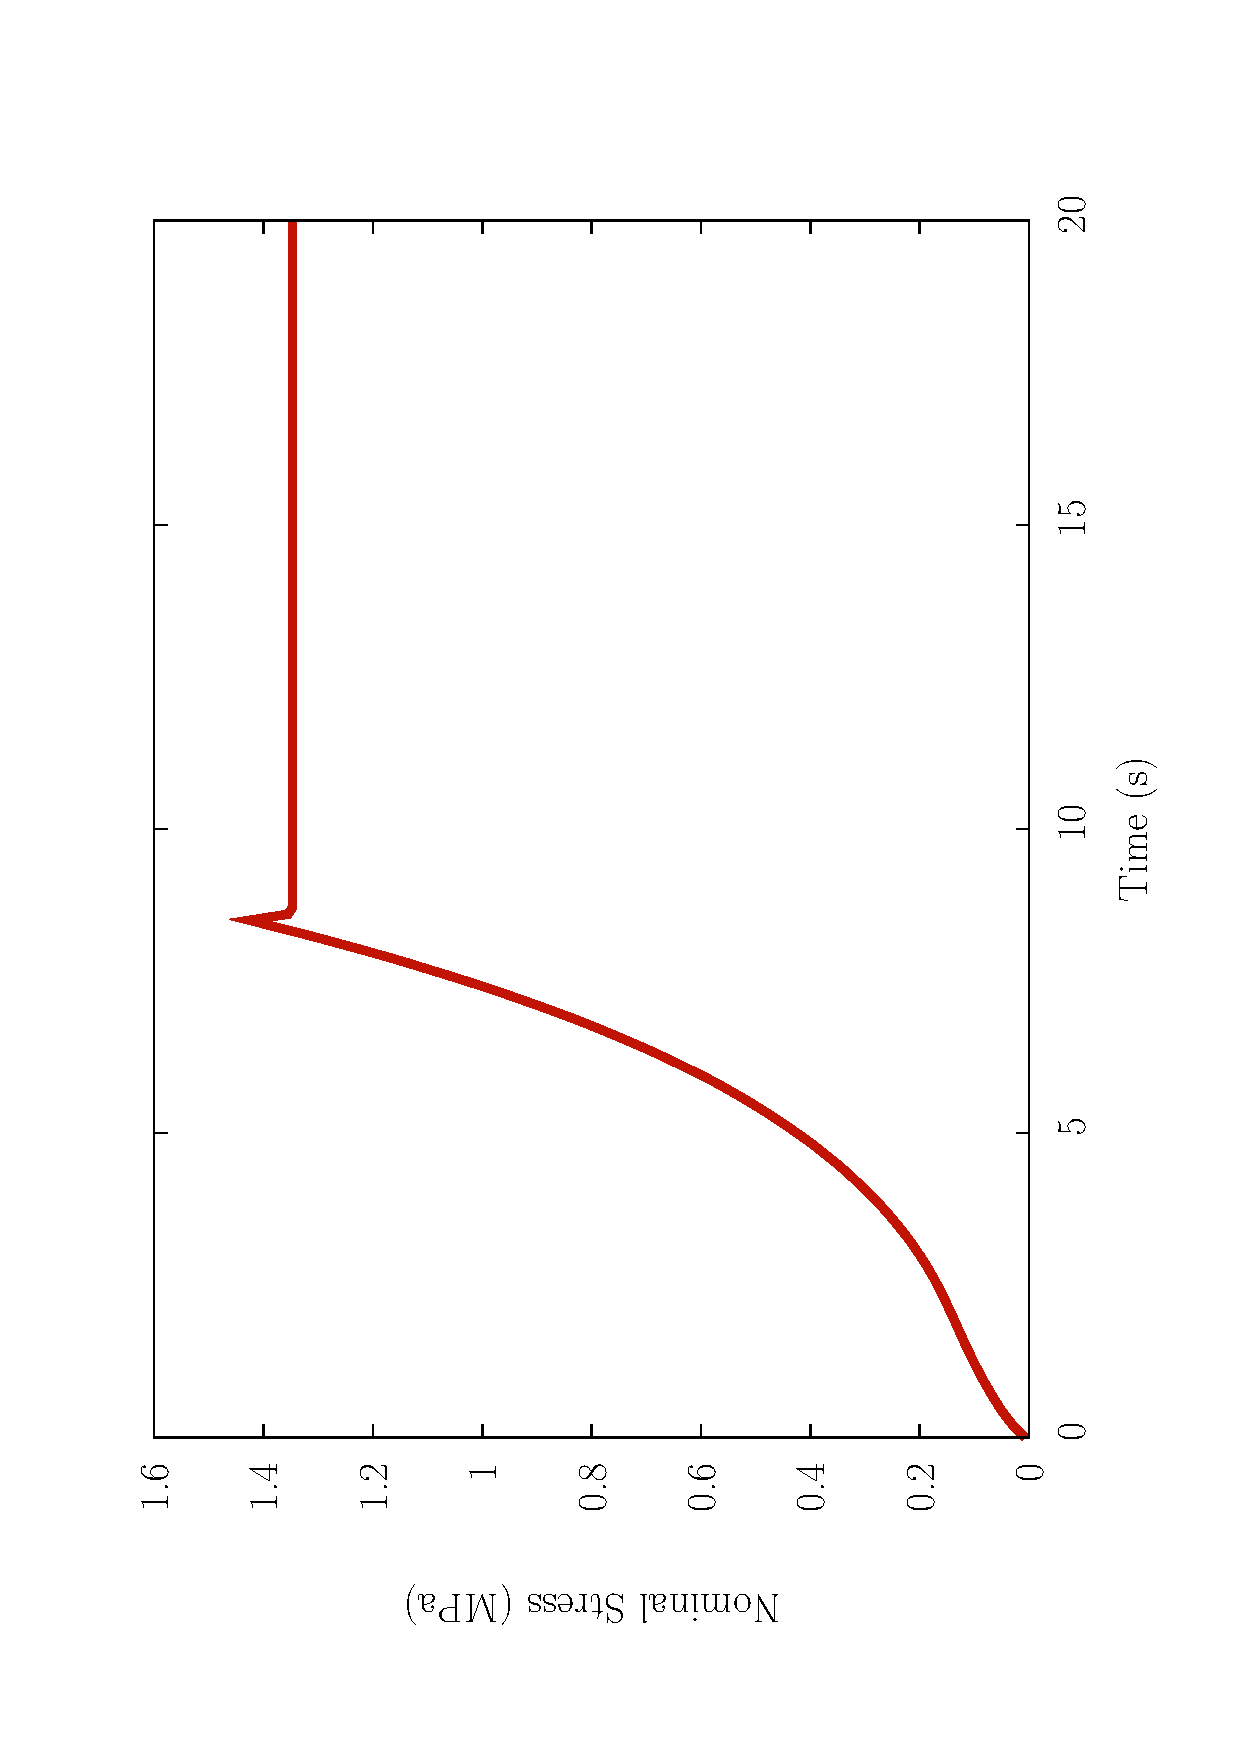
\includegraphics[width=0.6\textwidth,angle=270]{images/examples/%
    eulerian/pulling/plots/poro-elastic/poro-stress-relax-0p01}
  \caption{Quasistatic poroelastic model, $\dot{\epsilon}=0.01$ Hz,
    $D=1.037$ MPa.s.mm$^{-2}$.}
  \label{poro-stress-relax-0p01}
\end{figure}

\begin{figure}[!hptb]
  \centering
  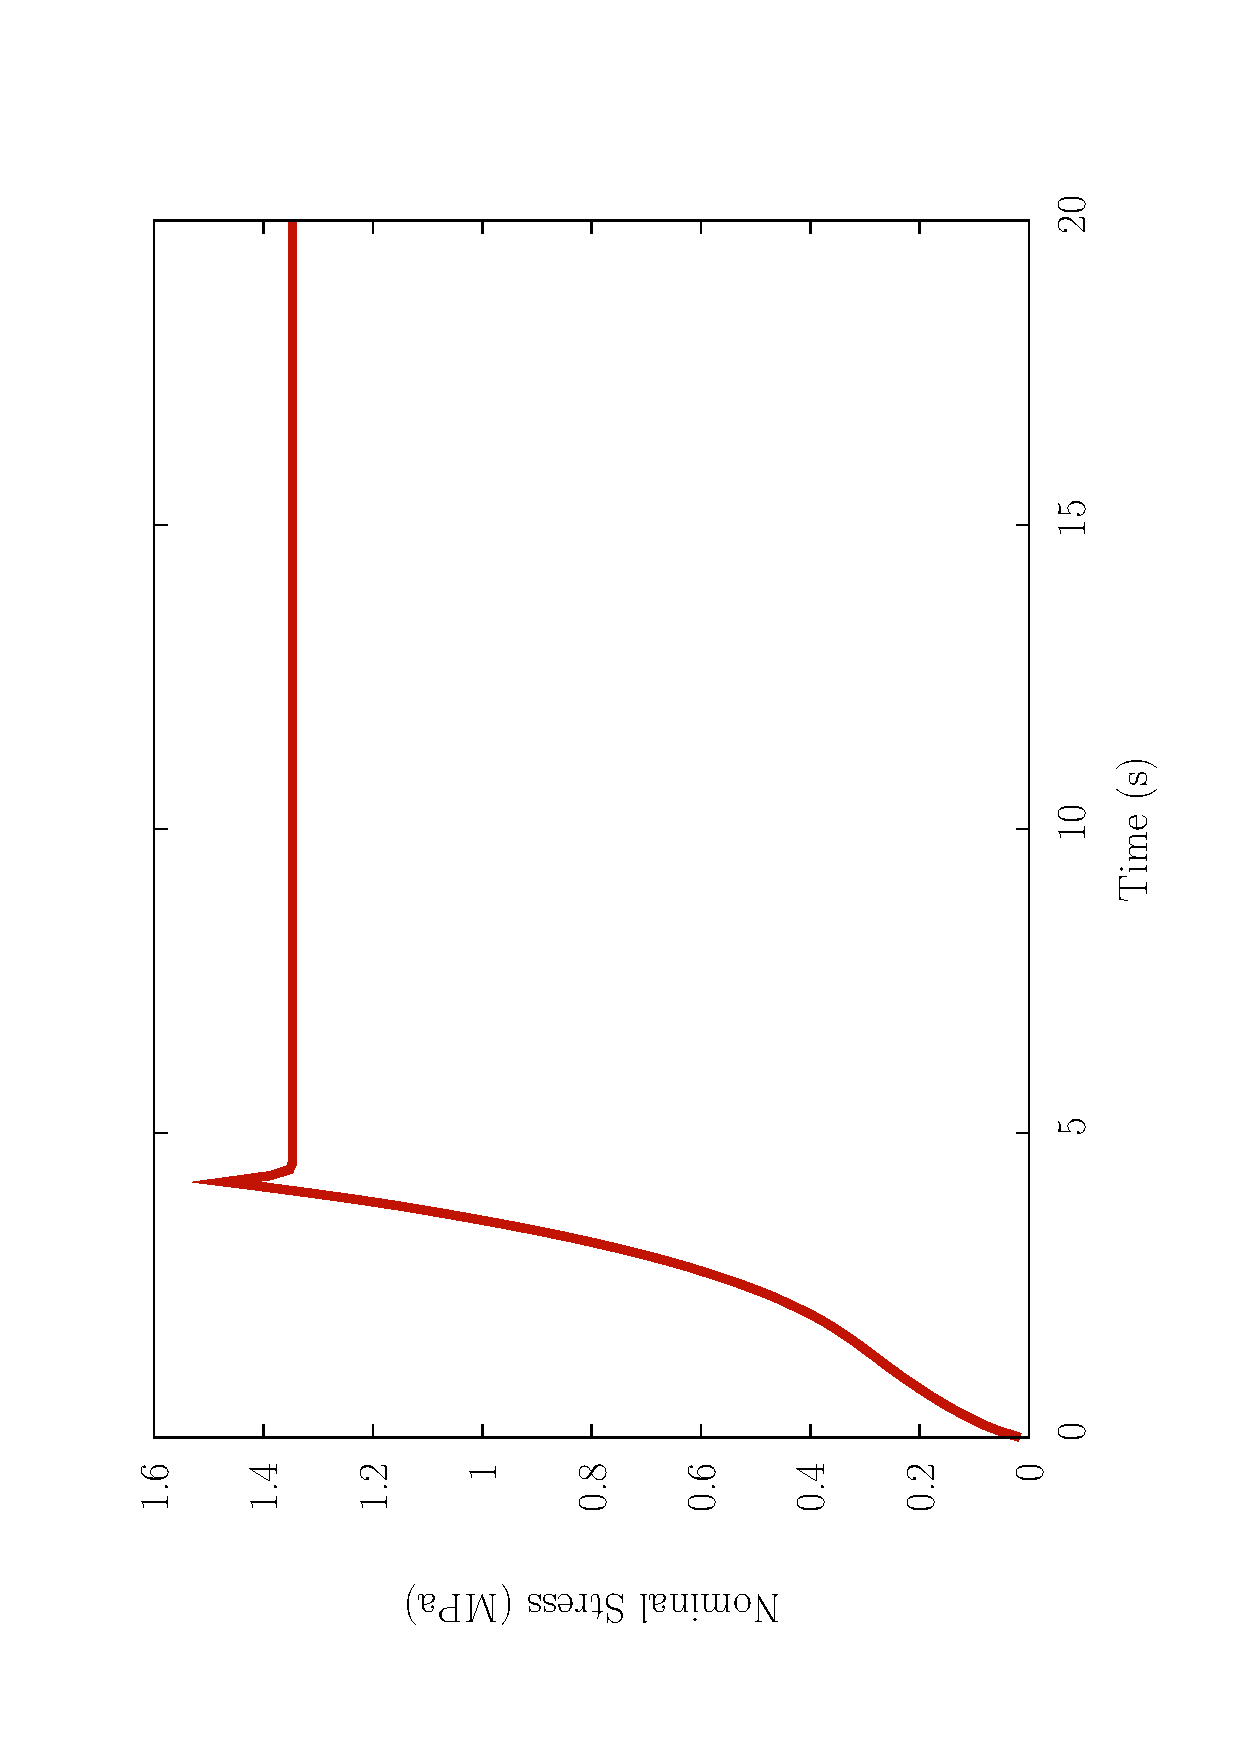
\includegraphics[width=0.6\textwidth,angle=270]{images/examples/%
    eulerian/pulling/plots/poro-elastic/poro-stress-relax-0p02}
  \caption{Quasistatic poroelastic model, $\dot{\epsilon}=0.02$ Hz,
    $D=1.037$ MPa.s.mm$^{-2}$.}
  \label{poro-stress-relax-0p02}
\end{figure}

\begin{figure}[!hptb]
  \centering
  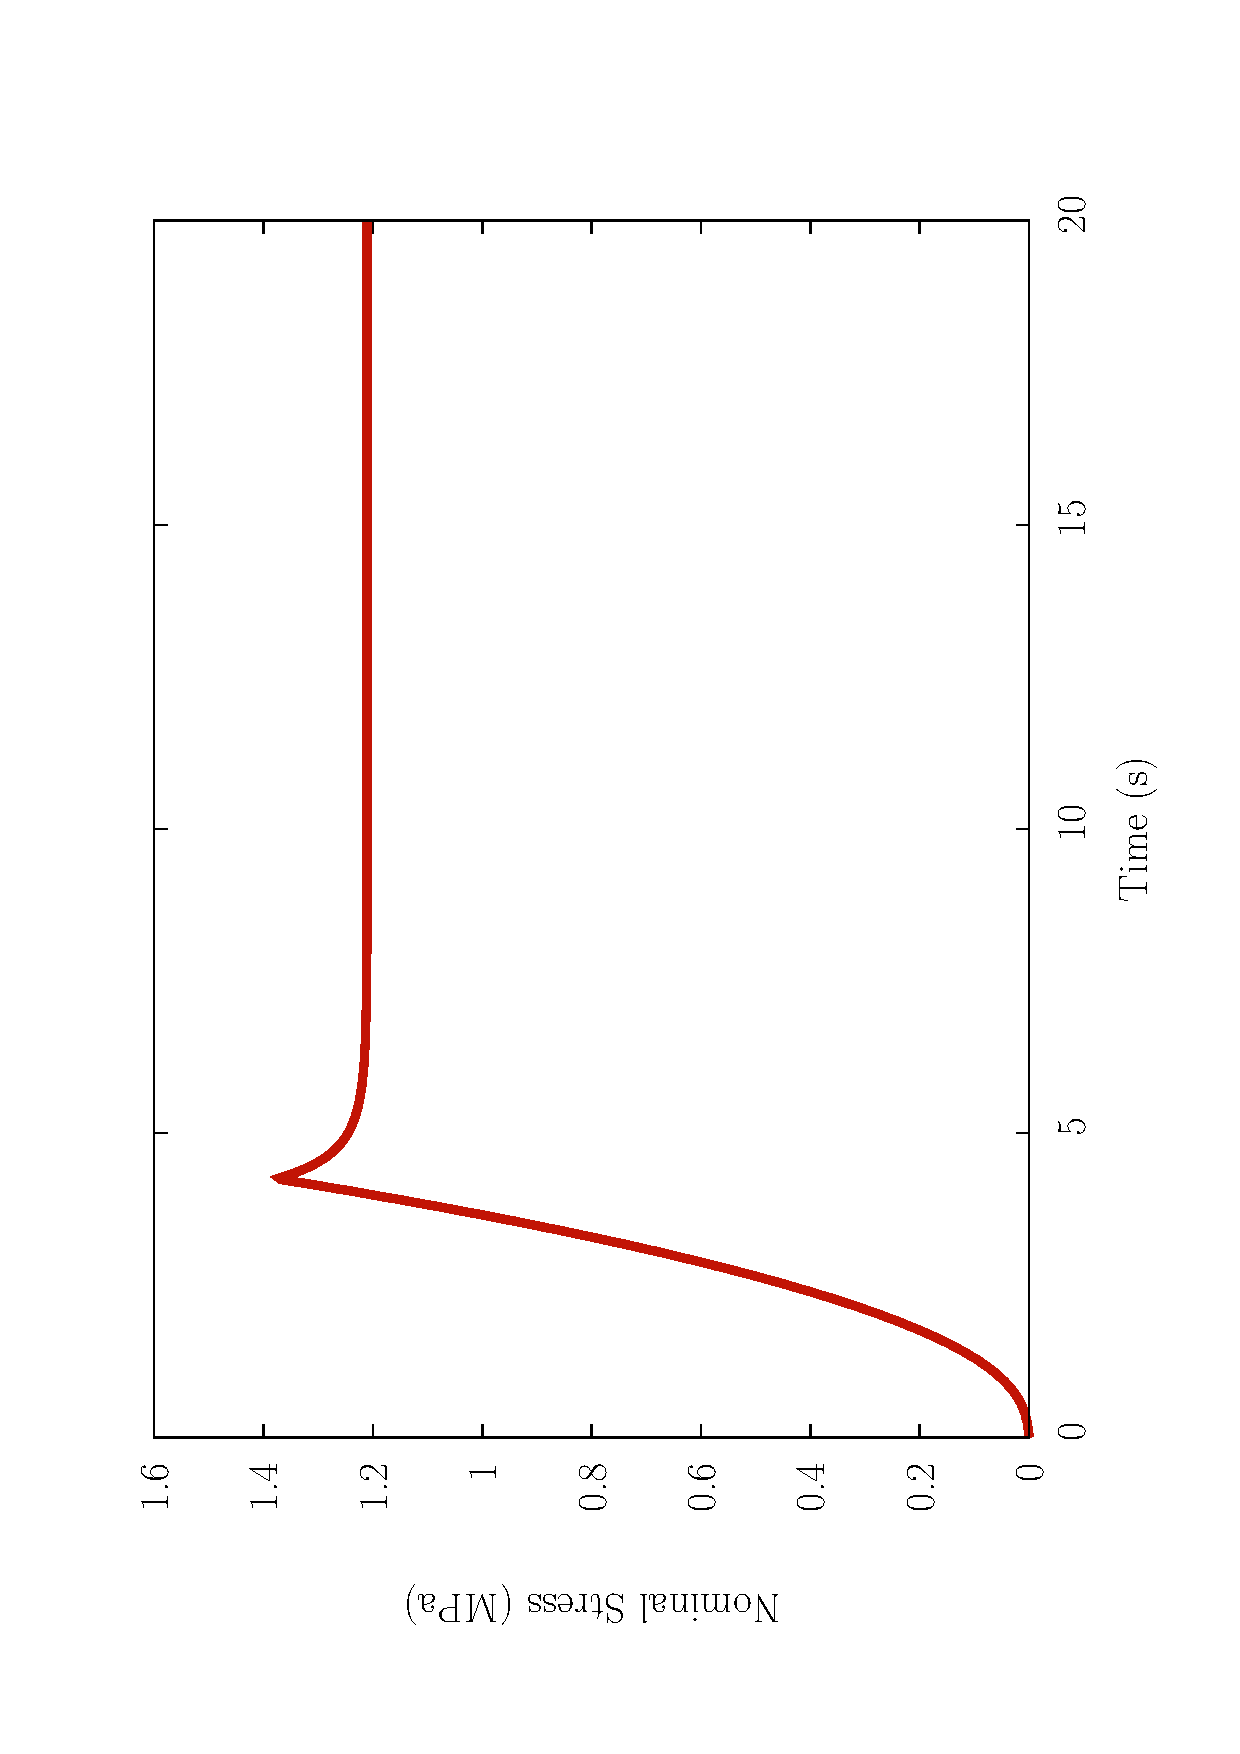
\includegraphics[width=0.6\textwidth,angle=270]{images/examples/%
    eulerian/pulling/plots/visco-elastic/visco-stress-relax-0p02-t0p3}
  \caption{Dynamic viscoelastic model, $\dot{\epsilon}=0.02$ Hz,
    $\tau=0.3$ s.}
  \label{visco-stress-relax-0p02-t0p3}
\end{figure}

\subsection{Hysteresis in the cyclic stress-strain response}
\label{hysteresis}

The examples in this section study the hysteresis in the stress-strain
response when the model is subjected to a complete load-unload
cycle. As before, for the solid phase, the boundary conditions specify
that one of longitudinal edges of the tissue is held fixed, while
subjecting the other to the suitable displacement load. The lateral
edges of the solid remain traction free. For the fluid, there is no
flow relative to the solid at the longitudinal edges, i.e.,
$\bv^{\mathrm{f}} = \bv^{\mathrm{c}}$. The lateral edges expose the
fluid to the bath, and therefore the fluid pressure is equated to that
of the bath, 0~MPa, along those edges.

In all these tests, the model was first loaded to a maximum strain of
0.085 (to match the experimental data presented in Figure~\ref%
{explanted-ligament}) and subsequently unloaded to no strain. Since
the numerical experiments so far have suggested conspicuous
differences between the quasistatic and dynamic solutions, both these
cases have been explored in this section. When the fluid flow fields
are observed during the course of these load-unload tests, it is found
that they constantly lag behind the motion of the solid; and it is
this relative velocity, and the corresponding frictional interaction
between the phases, that leads to energy dissipation manifesting
itself as the hysteresis loop.

For the quasistatic hysteresis curve presented in
Figure~\ref{medium-hysteresis-static-0p01-d1p037}, the model was
loaded at a rate of $\dot{\epsilon}=0.01$ Hz for 8.5~s to a total
strain of 0.085, and then subsequently unloaded at the same rate back
to 0 strain in another 8.5~s. This discontinuous (in time) velocity
boundary condition for the fluid is acceptable for the quasistatic
calculation. When compared to the hysteresis result arising from the
dynamic calculation loaded and unloaded at the same {\em average}
strain rate (Figure~\ref{medium-hysteresis-dynamic-0p01-d1p037}),%
\footnote{Since the uniform strain rate load-unload displacement
  condition prescribed for the quasistatic calculation (termed the
  {\em triangular load}) is insufficiently smooth in time, the dynamic
  calculations are instead subjected to a load-unload displacement
  that takes the shape of a cosine curve. This displacement condition
  reaches the same maximum strain and unloads to no strain at the same
  times as the triangular load, but maintains the necessary smoothness
  in the velocity fields to allow for dynamic calculations.} it is
clear once more that the quasistatic calculation lacks the
characteristic oscillations arising from pressure wave propagation in
the fluid observed in the dynamic calculation. It is also interesting
to note that beyond a certain strain, the solid is stiff enough to
overcome the oscillatory effects arising from the fluid flow.

When this average strain rate is decreased to $\bar{\dot{\epsilon}} =
0.001$ Hz, (1/10$^\mathrm{th}$ the rate of the preceding calculation),
the relative velocity between the phases correspondingly decreases,
resulting in reduced dissipation and area of the hysteresis loop
(see Figure~\ref{medium-hysteresis-dynamic-0p001-d1p037}). In other
words, this slower process proceeds closer to thermodynamic
equilibrium. In an analogous comparison, when the average strain rate
is maintained at $\bar{\dot{\epsilon}} = 0.01$ Hz, but the magnitude
of the frictional coefficient tensor is increased by a factor of 10 to
$D=10.37$ MPa.s.mm$^{-2}$, it is observed that the dynamic effects of
the fluid flow are much more prominent (as observed in
Figure~\ref{medium-hysteresis-dynamic-0p01-d10p37}). This is because
the comparable strain rates ensure similar relative velocities between
the phases (in the calculations corresponding to
Figures~\ref{medium-hysteresis-dynamic-0p01-d1p037} and
\ref{medium-hysteresis-dynamic-0p01-d10p37}), but the frictional
interaction between the fluid and solid phases has now scaled by this
factor of 10.

The results presented in this section demonstrate aspects of the
experimentally observed mechanical response of ligaments seen in
Figure~\ref{explanted-ligament}. Finally, the biphasic poroelastic
results presented in this section are compared to the response of the
purely linear viscoelastic model introduced in the preceding
section. This model was loaded at a strain rate of
$\dot{\epsilon}=0.01$ Hz for 8.5~s to a total strain of 0.085, and
then subsequently unloaded at the same rate back to 0 strain in
another 8.5~s. The resulting stress-strain curve is shown in
Figure~\ref{medium-hysteresis-visco-0p01-t0p3}. Upon comparing it with
Figure~\ref{medium-hysteresis-dynamic-0p01-d1p037}, we find as we did
before that, stemming from initial frictional interaction between the
phases, the poroelastic case starts out stiffer, and the viscoelastic
model fails to capture any of the dynamic effects arising from the
fluid flow.

\begin{figure}[!hptb]
\centering
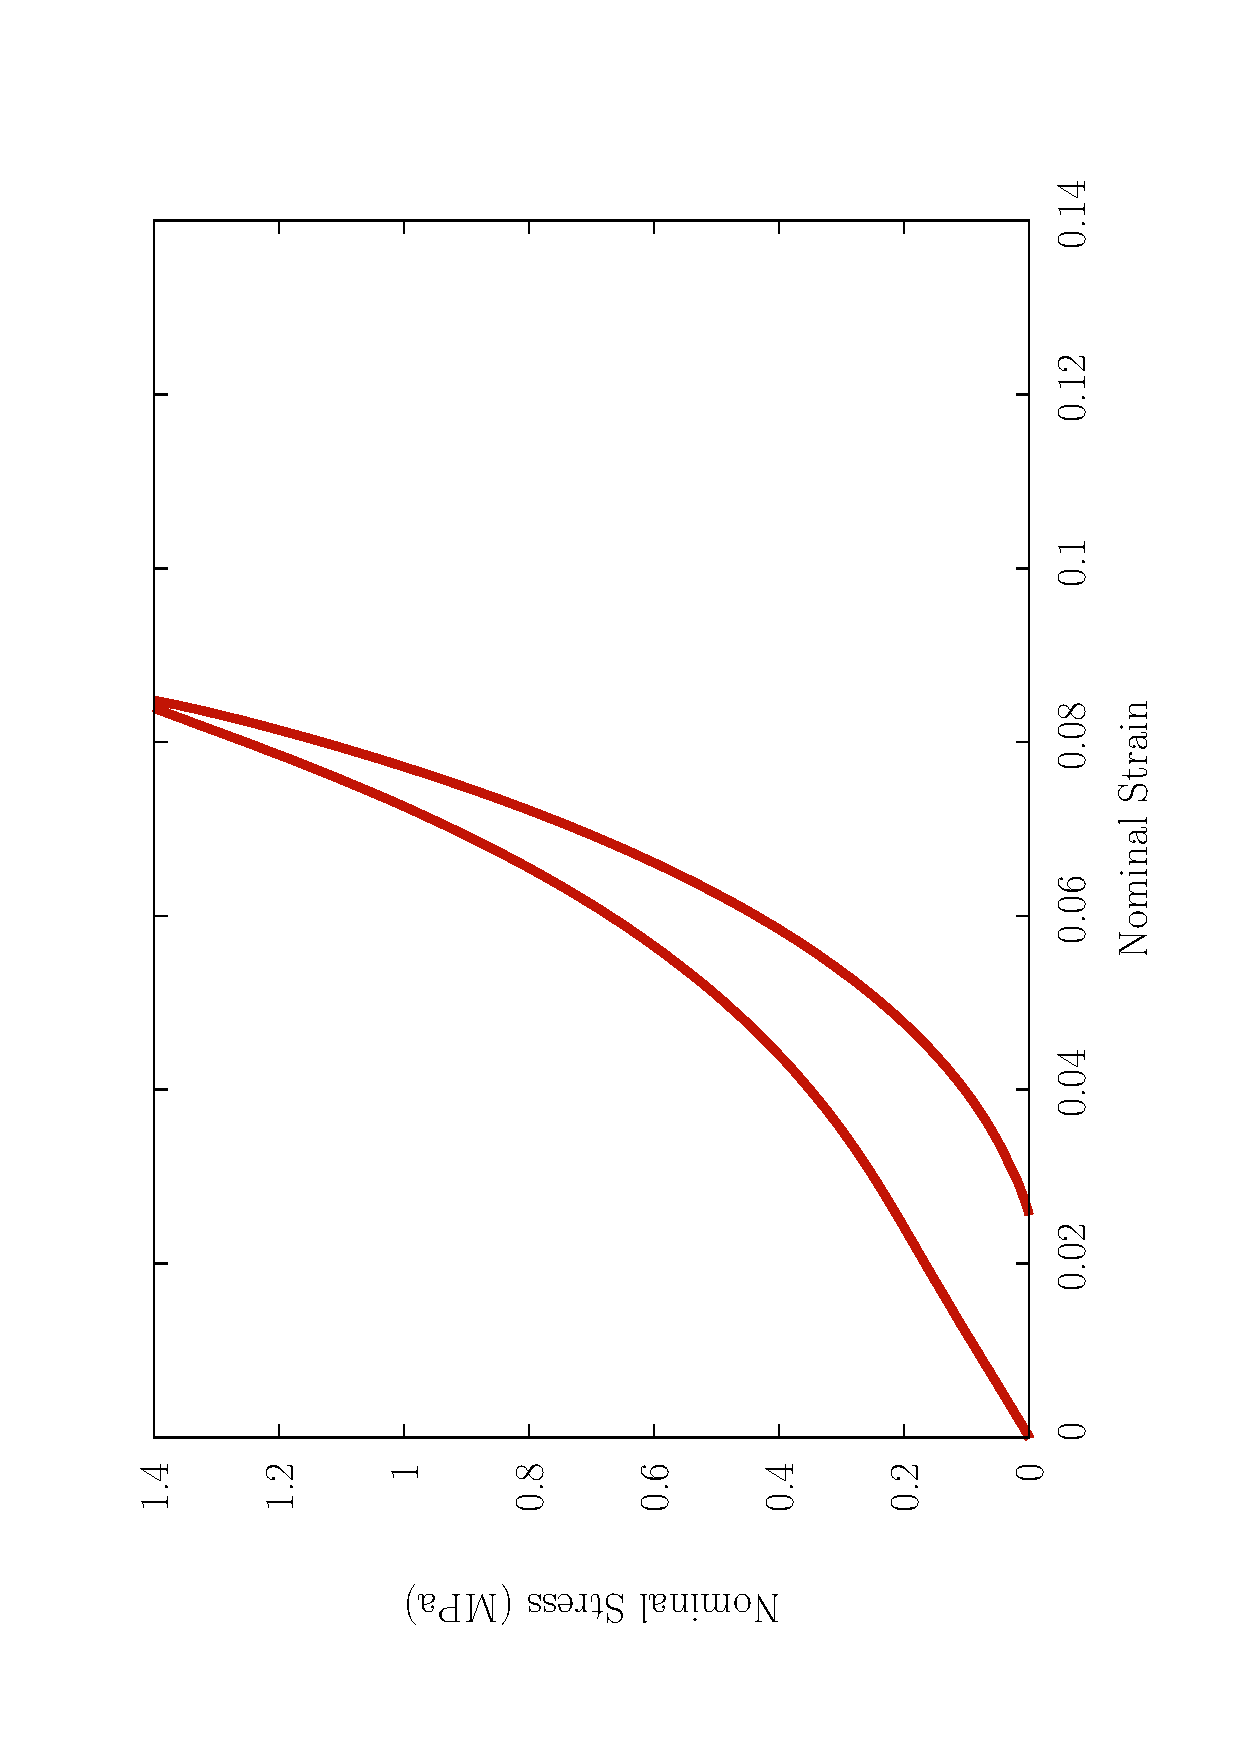
\includegraphics[width=0.6\textwidth,angle=270]{images/examples/%
eulerian/pulling/plots/poro-elastic/medium-hysteresis-static-0p01-d1p037}
\caption{Quasistatic poroelastic model, $\dot{\epsilon}=0.01$ Hz, $D=1.037$
  MPa.s.mm$^{-2}$.}
\label{medium-hysteresis-static-0p01-d1p037}
\end{figure}

\begin{figure}[!hptb]
\centering
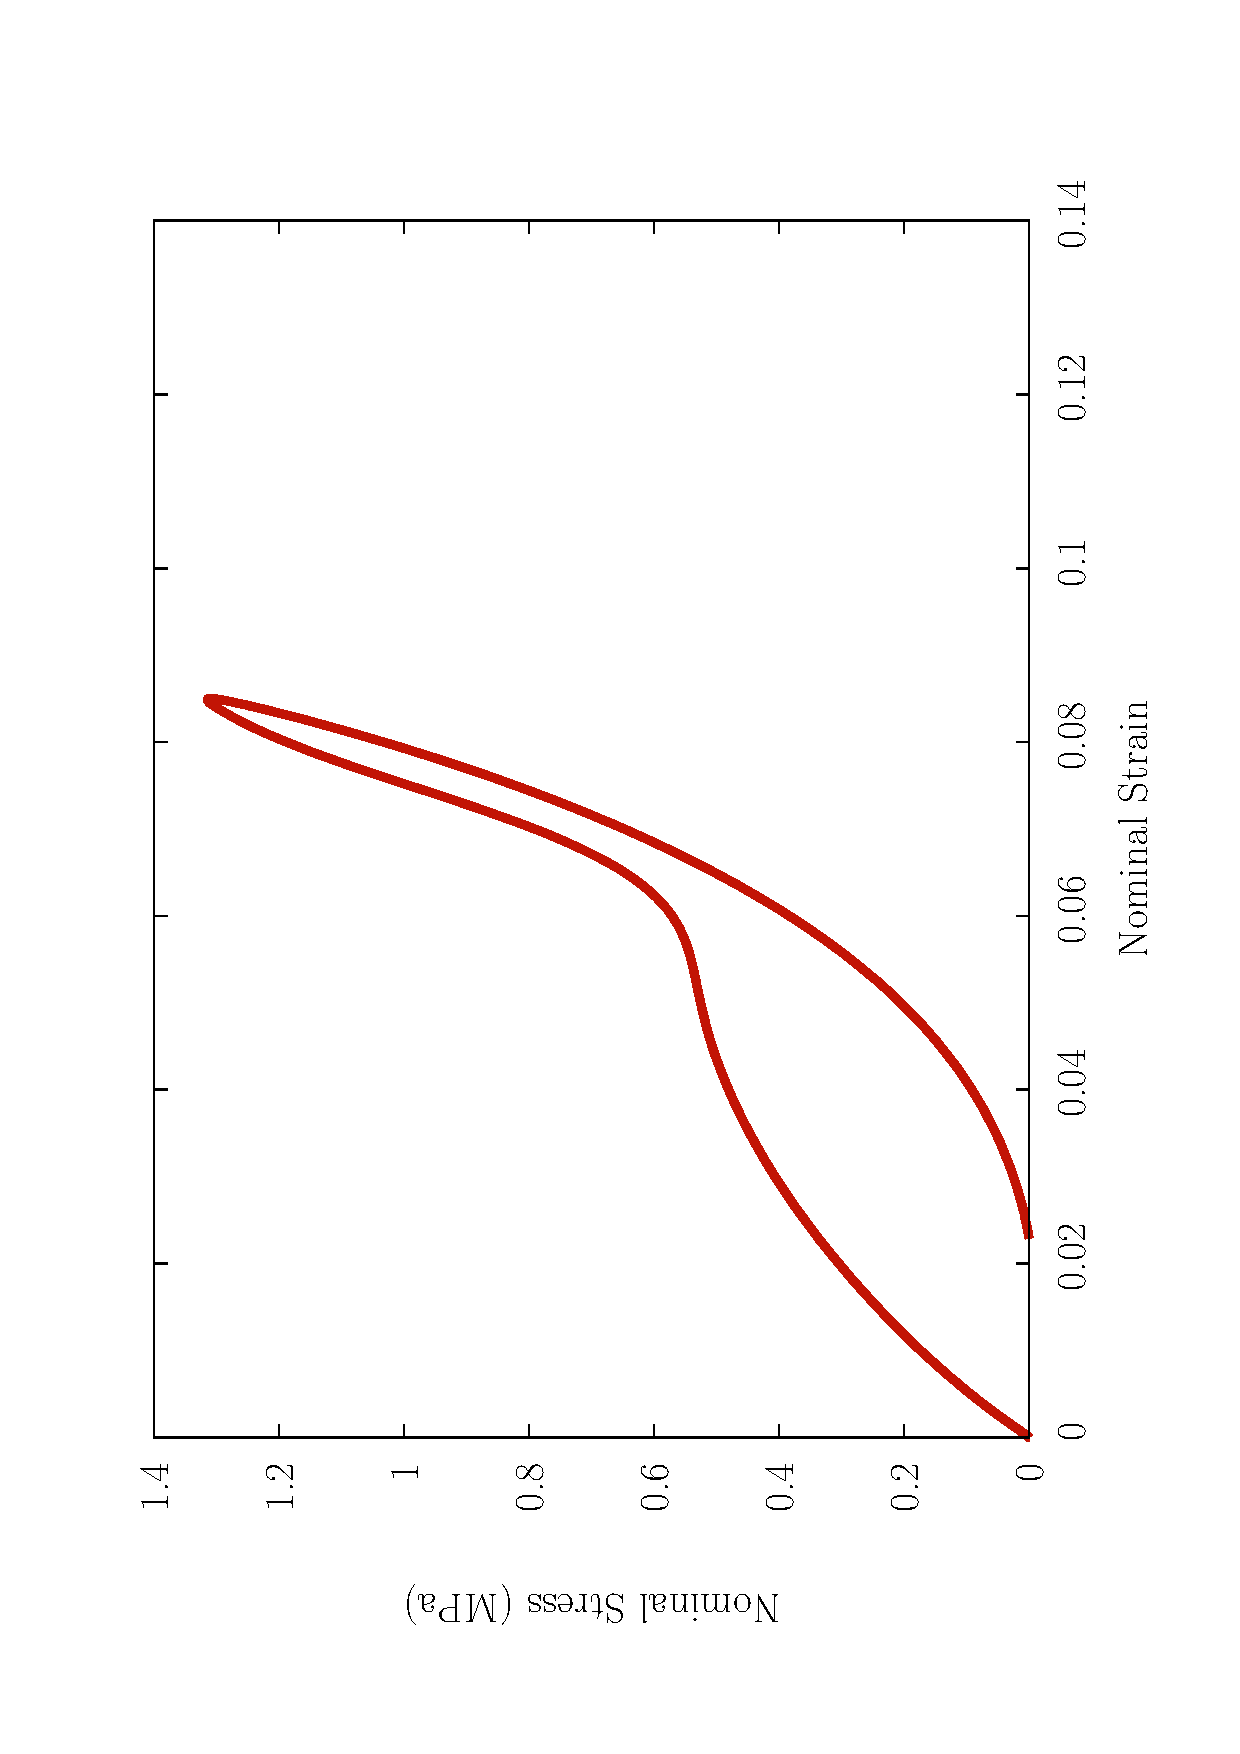
\includegraphics[width=0.6\textwidth,angle=270]{images/examples/%
eulerian/pulling/plots/poro-elastic/medium-hysteresis-dynamic-0p01-d1p037}
\caption{Dynamic poroelastic model, $\bar{\dot{\epsilon}}=0.01$ Hz,
  $D=1.037$ MPa.s.mm$^{-2}$.}
\label{medium-hysteresis-dynamic-0p01-d1p037}
\end{figure}

\begin{figure}[!hptb]
\centering
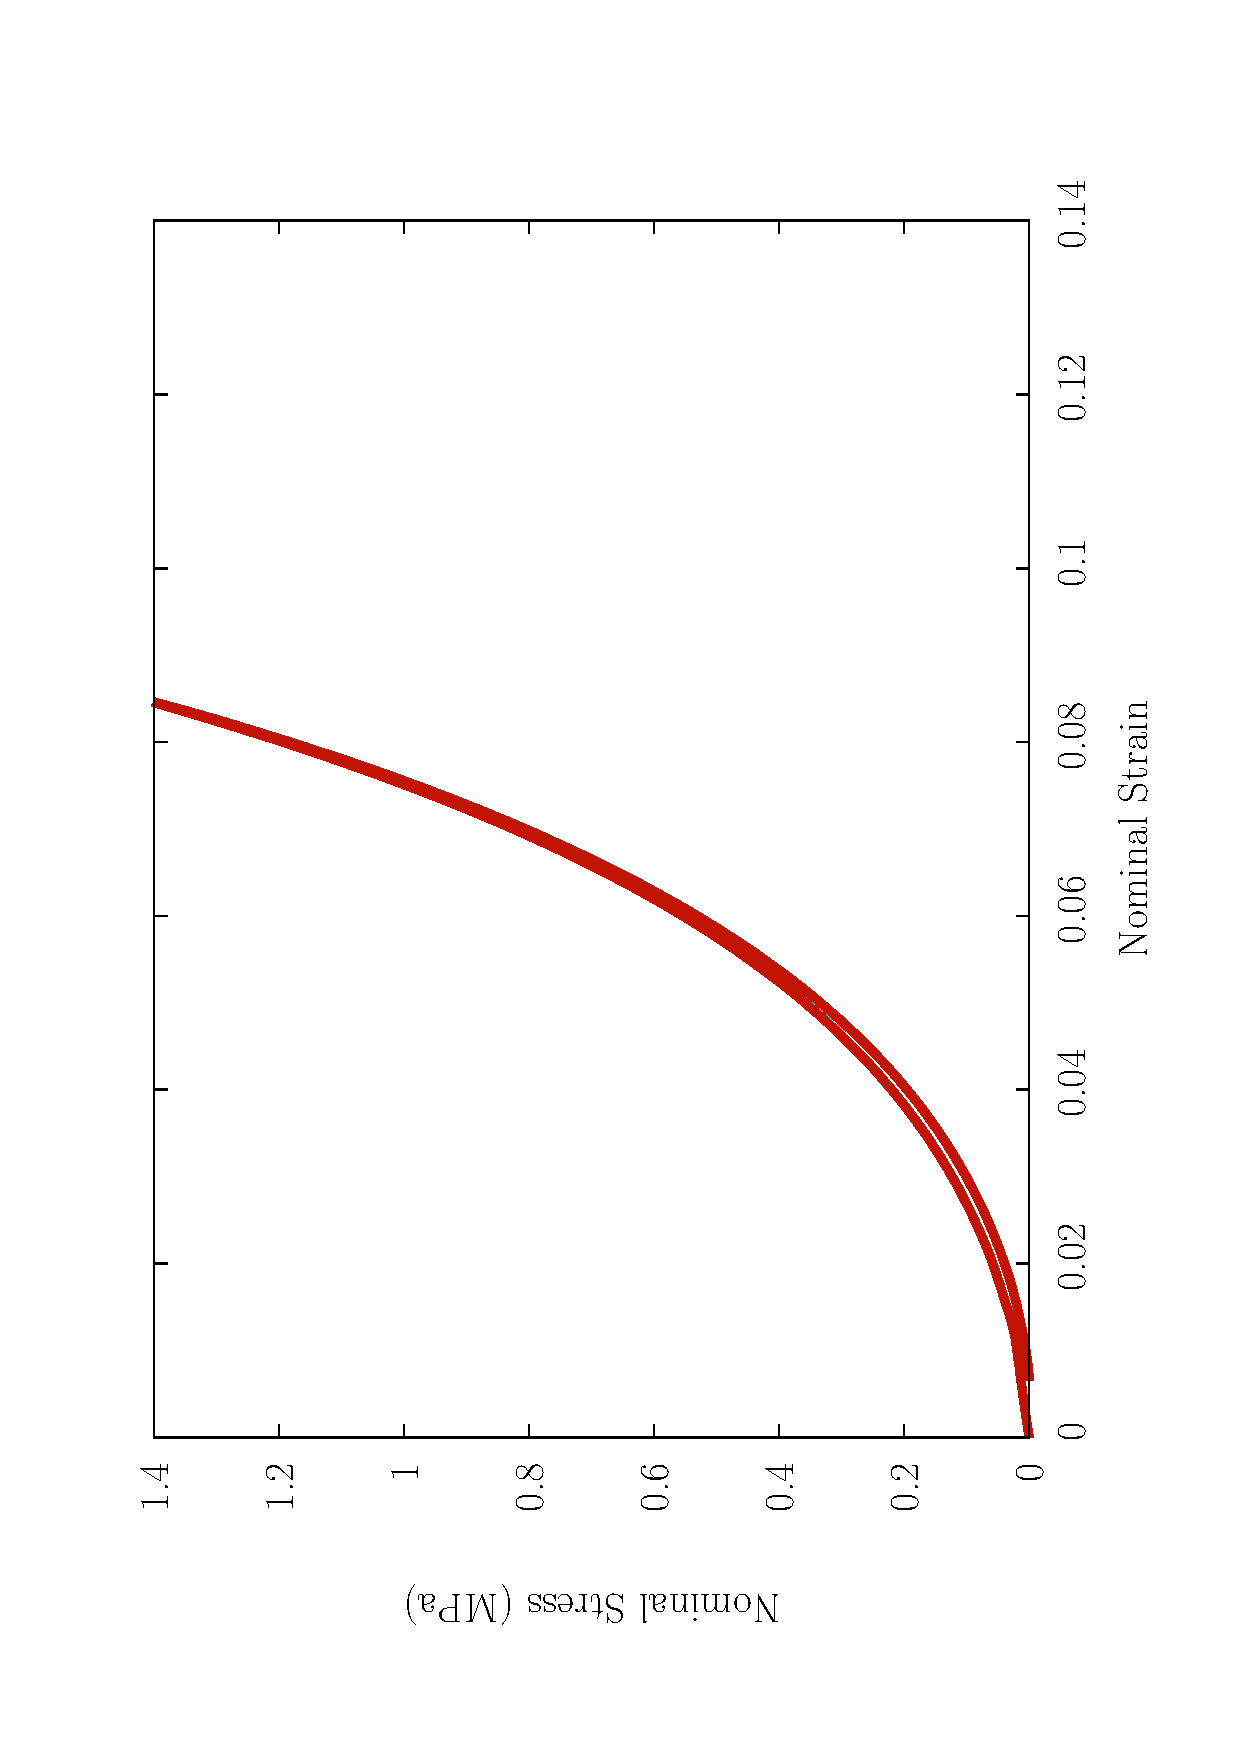
\includegraphics[width=0.6\textwidth,angle=270]{images/examples/%
eulerian/pulling/plots/poro-elastic/medium-hysteresis-dynamic-0p001-d1p037}
\caption{Dynamic poroelastic model, $\bar{\dot{\epsilon}}=0.001$ Hz,
  $D=1.037$ MPa.s.mm$^{-2}$.}
\label{medium-hysteresis-dynamic-0p001-d1p037}
\end{figure}

\begin{figure}[!hptb]
\centering
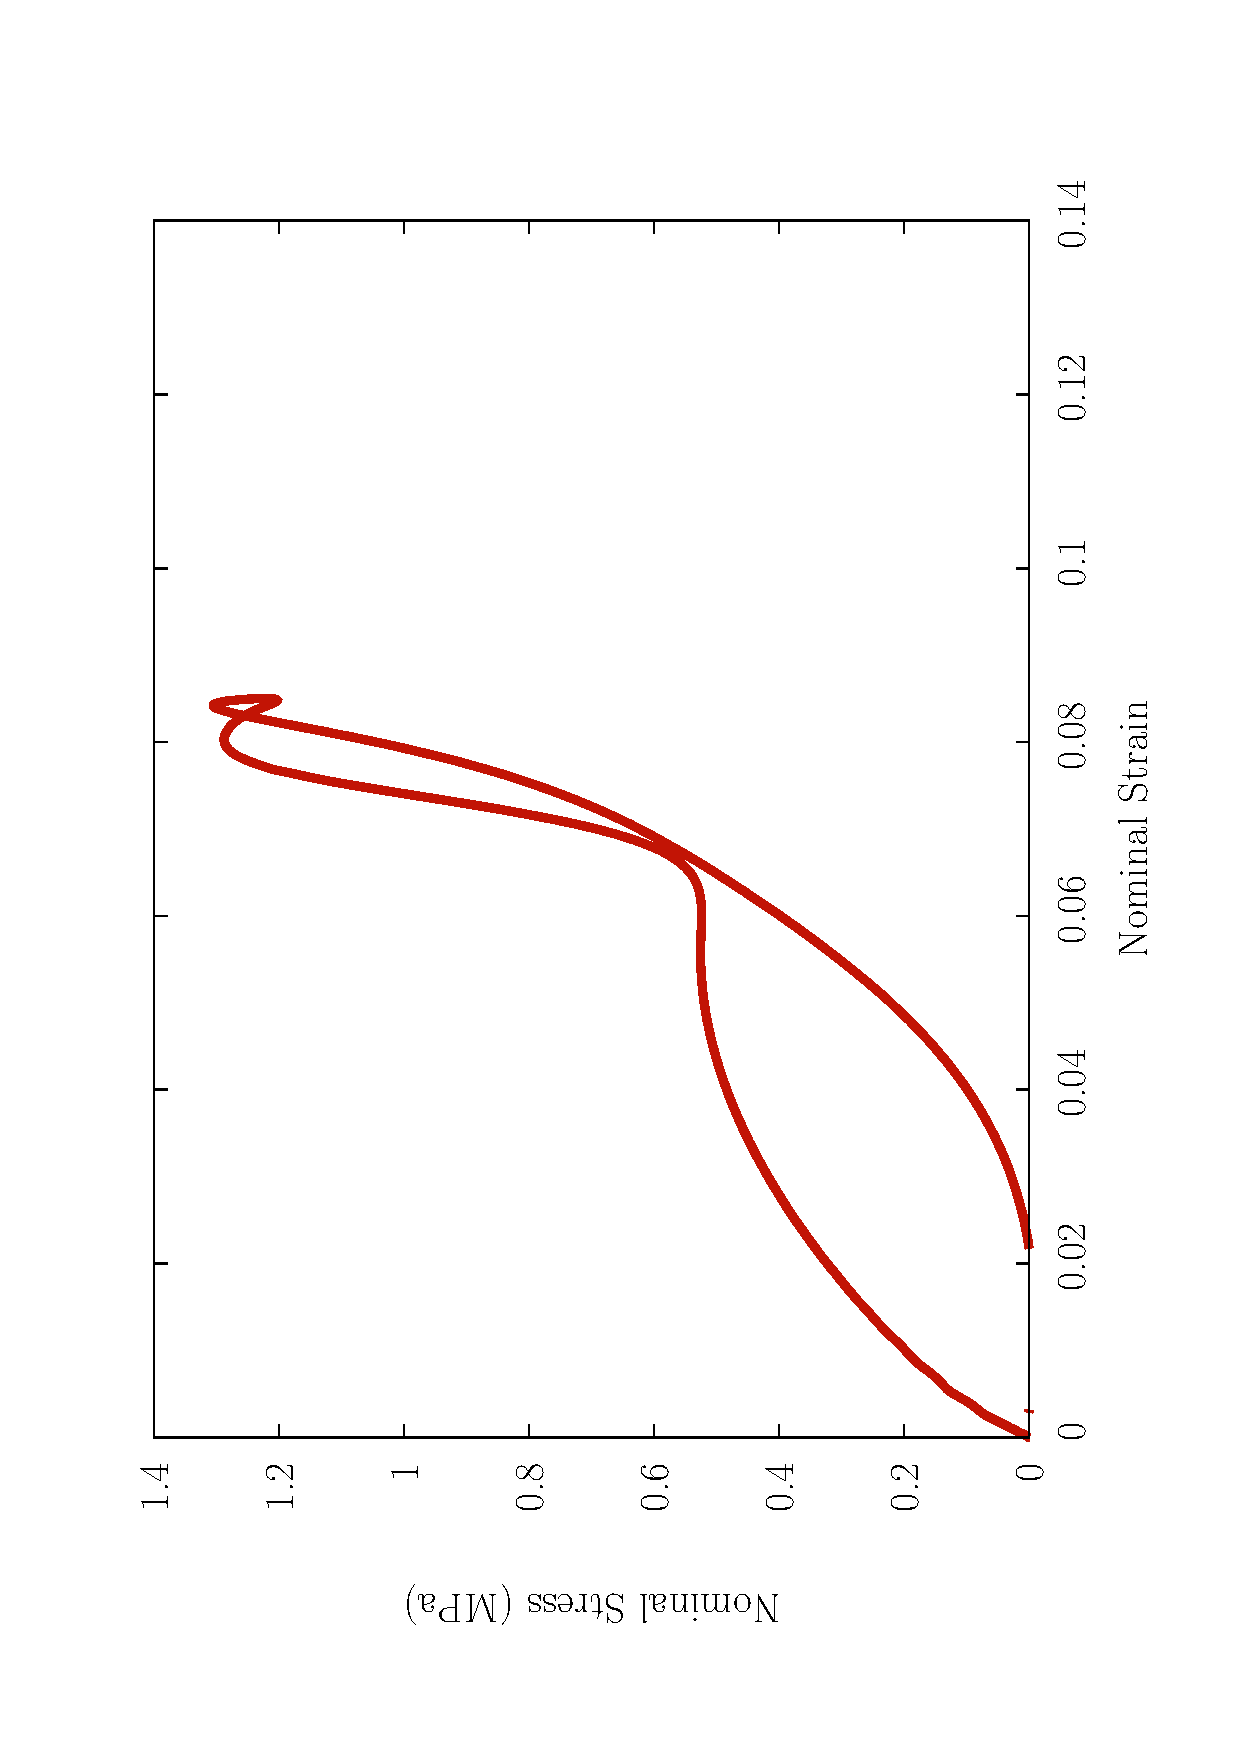
\includegraphics[width=0.6\textwidth,angle=270]{images/examples/%
eulerian/pulling/plots/poro-elastic/medium-hysteresis-dynamic-0p01-d10p37}
\caption{Dynamic poroelastic model, $\bar{\dot{\epsilon}}=0.01$ Hz,
  $D=10.37$ MPa.s.mm$^{-2}$.}
\label{medium-hysteresis-dynamic-0p01-d10p37}
\end{figure}

\begin{figure}[!hptb]
\centering
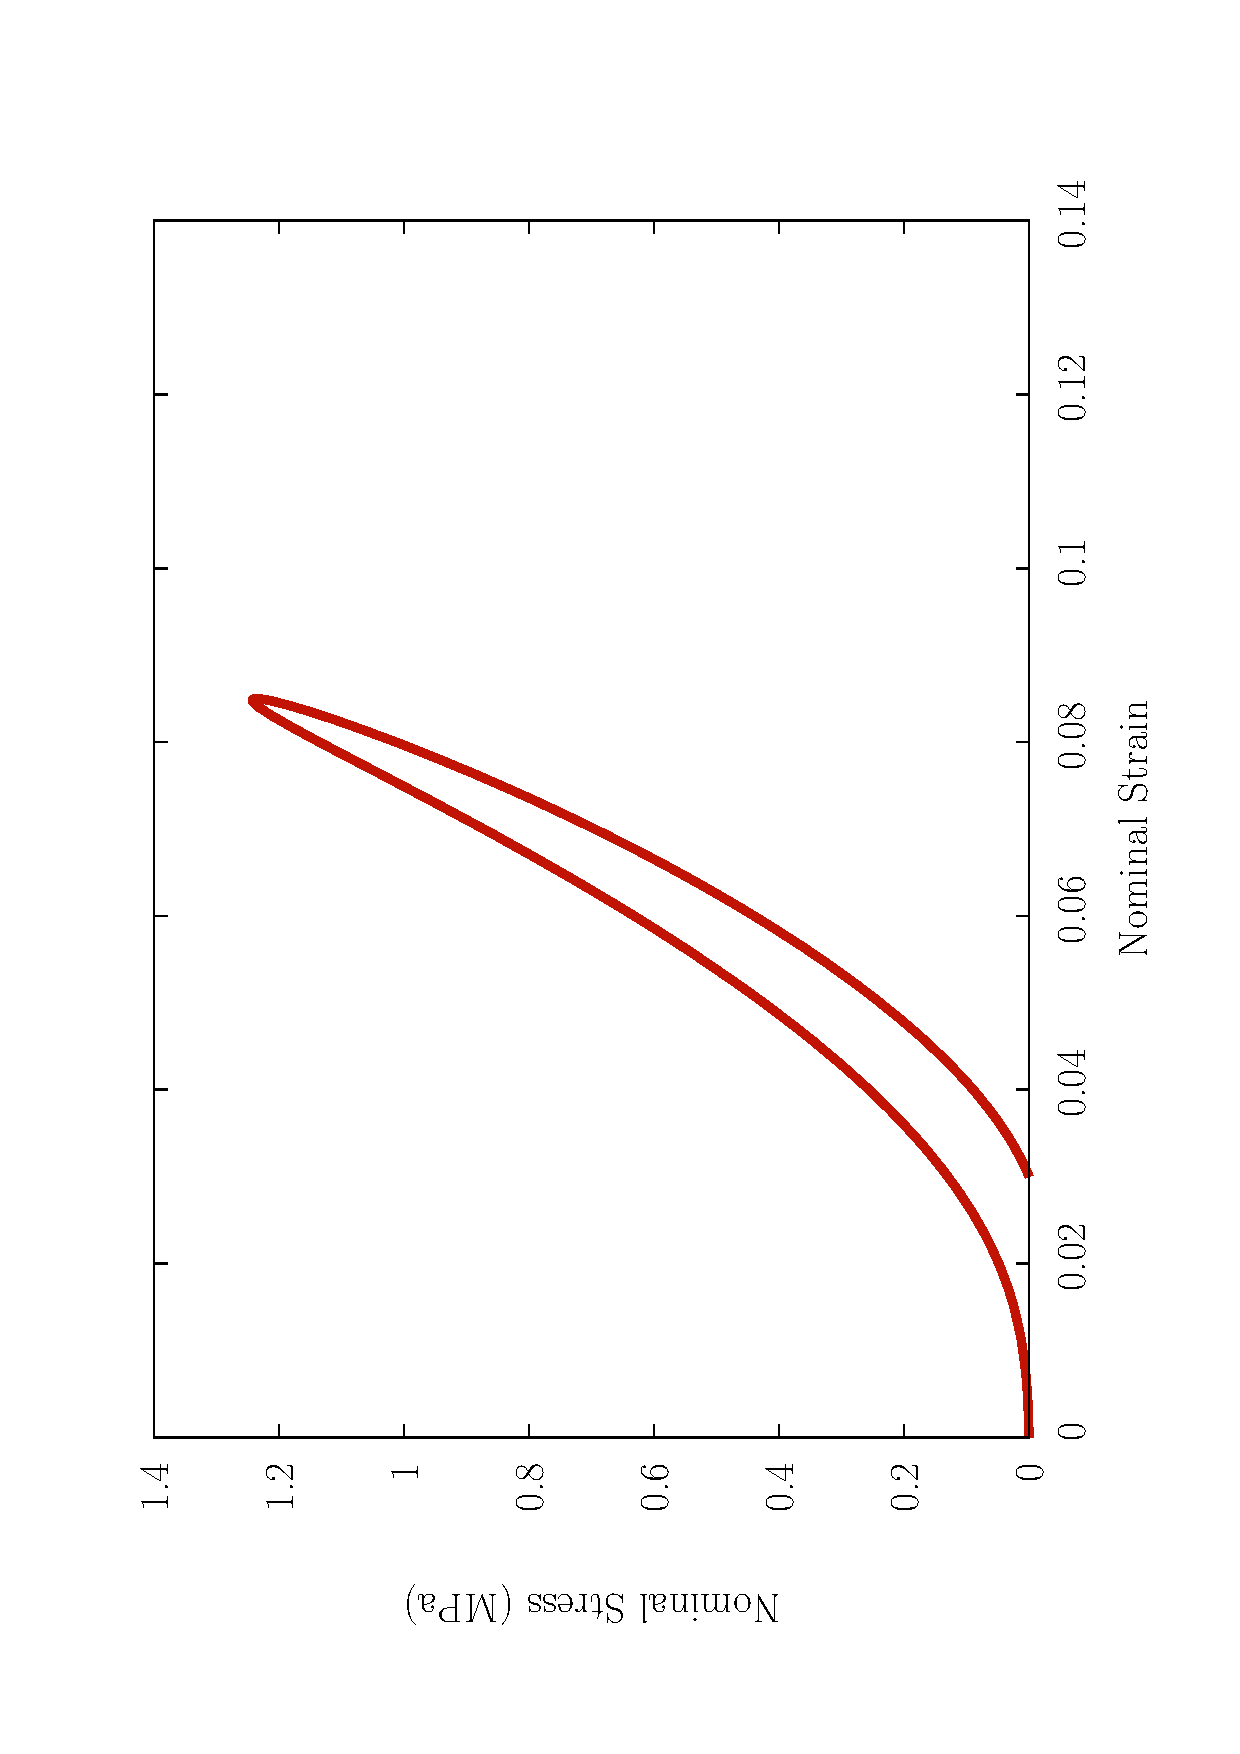
\includegraphics[width=0.6\textwidth,angle=270]{images/examples/%
eulerian/pulling/plots/visco-elastic/medium-hysteresis-visco-0p01-t0p3}
\caption{Dynamic viscoelastic model, $\dot{\epsilon}=0.01$ Hz,
  $\tau=0.3$ s.}
\label{medium-hysteresis-visco-0p01-t0p3}
\end{figure}

\section{Examining the effects of the mechanical environment on the
  growth of tumours}
\label{tumour-growth}

This final section presents a preliminary foray into tailoring the
mathematical formulation developed in Chapter~\ref{eulerian%
  -perspective} to studying the mechanics of growing tumours. Unlike
the computations presented in the preceding sections, which
principally focused on the biphasic mechanics of soft tissues in the
absence of biochemical interactions between the phases (tissue
growth), in examples that follow, we will turn our attention to an
idealisation of growing tumours, and examine the role of the
mechanical environment on its growth.

Similar to the approach followed in Section~\ref{simple-physics}, the
computations presented below serve only to demonstrate aspects of the
coupled physics underlying the problem, and the actual constitutive
modelling choices (and corresponding numerical parameters) chosen are
not intended for direct comparison with experiment. Incorporating more
realistic modelling choices (such as the use of more sophisticated
biochemistry involving additional species \citep{tjacks2000}), and the
ascertainment of corresponding parameters, is a direction for future
work.

The computations presented in this section are motivated by and aim to
replicate a fundamental experimental observation: Compressive solid
stress along a given direction restricts the in vitro growth of
tumours along that direction \citep{jain1997}. The foundational
examples discussed in Sections~\ref{tumour-isotropic-swelling}--%
\ref{cell-transport} focus on different aspects of this confined
tumour growth problem, and a combination of all these phenomena are
manifested in the final computation presented in
Section~\ref{cacophonous-medley}.

The computational model used in this section is primarily a solid
comprised of an extra-cellular matrix (ECM) and tumour cells capable
of moving with respect to this matrix.\footnote{We have already
  studied the effects of the extra-cellular fluid flow on the
  mechanics in some detail in the preceding sections. Since we are
  focusing on other phenomena in this section, we have chosen to
  ignore the fluid here.} It is assumed that the solute
phases, such as the nutrients and enzymes, are present in sufficient
amounts to drive the biochemistry that allows the cells to proliferate
and produce more ECM. The model geometry, as visualised in
Figure~\ref{tumour-isotropic-swelling-0}, is a semicircle and has a
radius of 10~mm initially.

\subsection{Kinematic swelling concomitant with growth}
\label{tumour-isotropic-swelling}

In this initial calculation, we focus on the kinematic swelling
associated with an increase in the mass of the solid tumour. The
isotropic swelling tensor introduced in
Section~\ref{kinematics-of-growth} has been modified to,

\begin{equation}
\bF^{\mathrm{g}^{\mathrm{c}}} = \left(
\begin{array}{ccc}
\left(\frac{\rho_0^{\mathrm{c}}}
     {\rho_{0_{\mathrm{ini}}}^{\mathrm{c}}}\right)^{1/2} & 0 & 0 \\ 0
     & \left(\frac{\rho_0^{\mathrm{c}}}
     {\rho_{0_{\mathrm{ini}}}^{\mathrm{c}}}\right)^{1/2} & 0 \\ 0 & 0
     & 1 \end{array} \right),
\label{2d-isotropic}
\end{equation}

\noindent since we are working in two dimensions under a plain strain
setting.

This example solves the mass (\ref{localbalanceofmass}) and momentum
balance (\ref{localbalanceofmomentum}) equations for the solid
(comprised at this point of both cells and the matrix) in the
reference configuration. The boundary conditions for the momentum
balance equations only prevent rigid body motion of the domain, and do
not constrain the constrain its deformation in anyway. The mass
balance equation is solved with a uniform source term
$\Pi^{\mathrm{c}}=0.001$~kg.m$^{-3}$/day. The initial solid
concentration is $\rho_{0_{\mathrm{ini}}}^{\mathrm{c}}=1~$kg.m$^{-3}$.

As a result of this uniform mass source, and the increasing solid
concentration, the domain begins to
swell. Figures~\ref{tumour-isotropic-swelling-0} and
\ref{tumour-isotropic-swelling-100} show the tumour
initially, and after 100 days. The colour contours provide the
radial displacement of the solid in mm, and the arrows provide the
direction of its velocity. Since there are no constraints on the
deformation, this swelling is
isotropic. Figure~\ref{tumour-isotropic-area-evolution}, shows the area of
the domain increasing linearly in time over the duration of the
computation. Note that the ratio of the final to initial areas
172.788~mm$^2$/157.08~mm$^2$ is exactly the same as the ratio of final
to initial concentrations 1.1~kg.m$^{-3}$/1~kg.m$^{-3}$, as one would
expect.

\begin{figure}[!hptb]
\centering
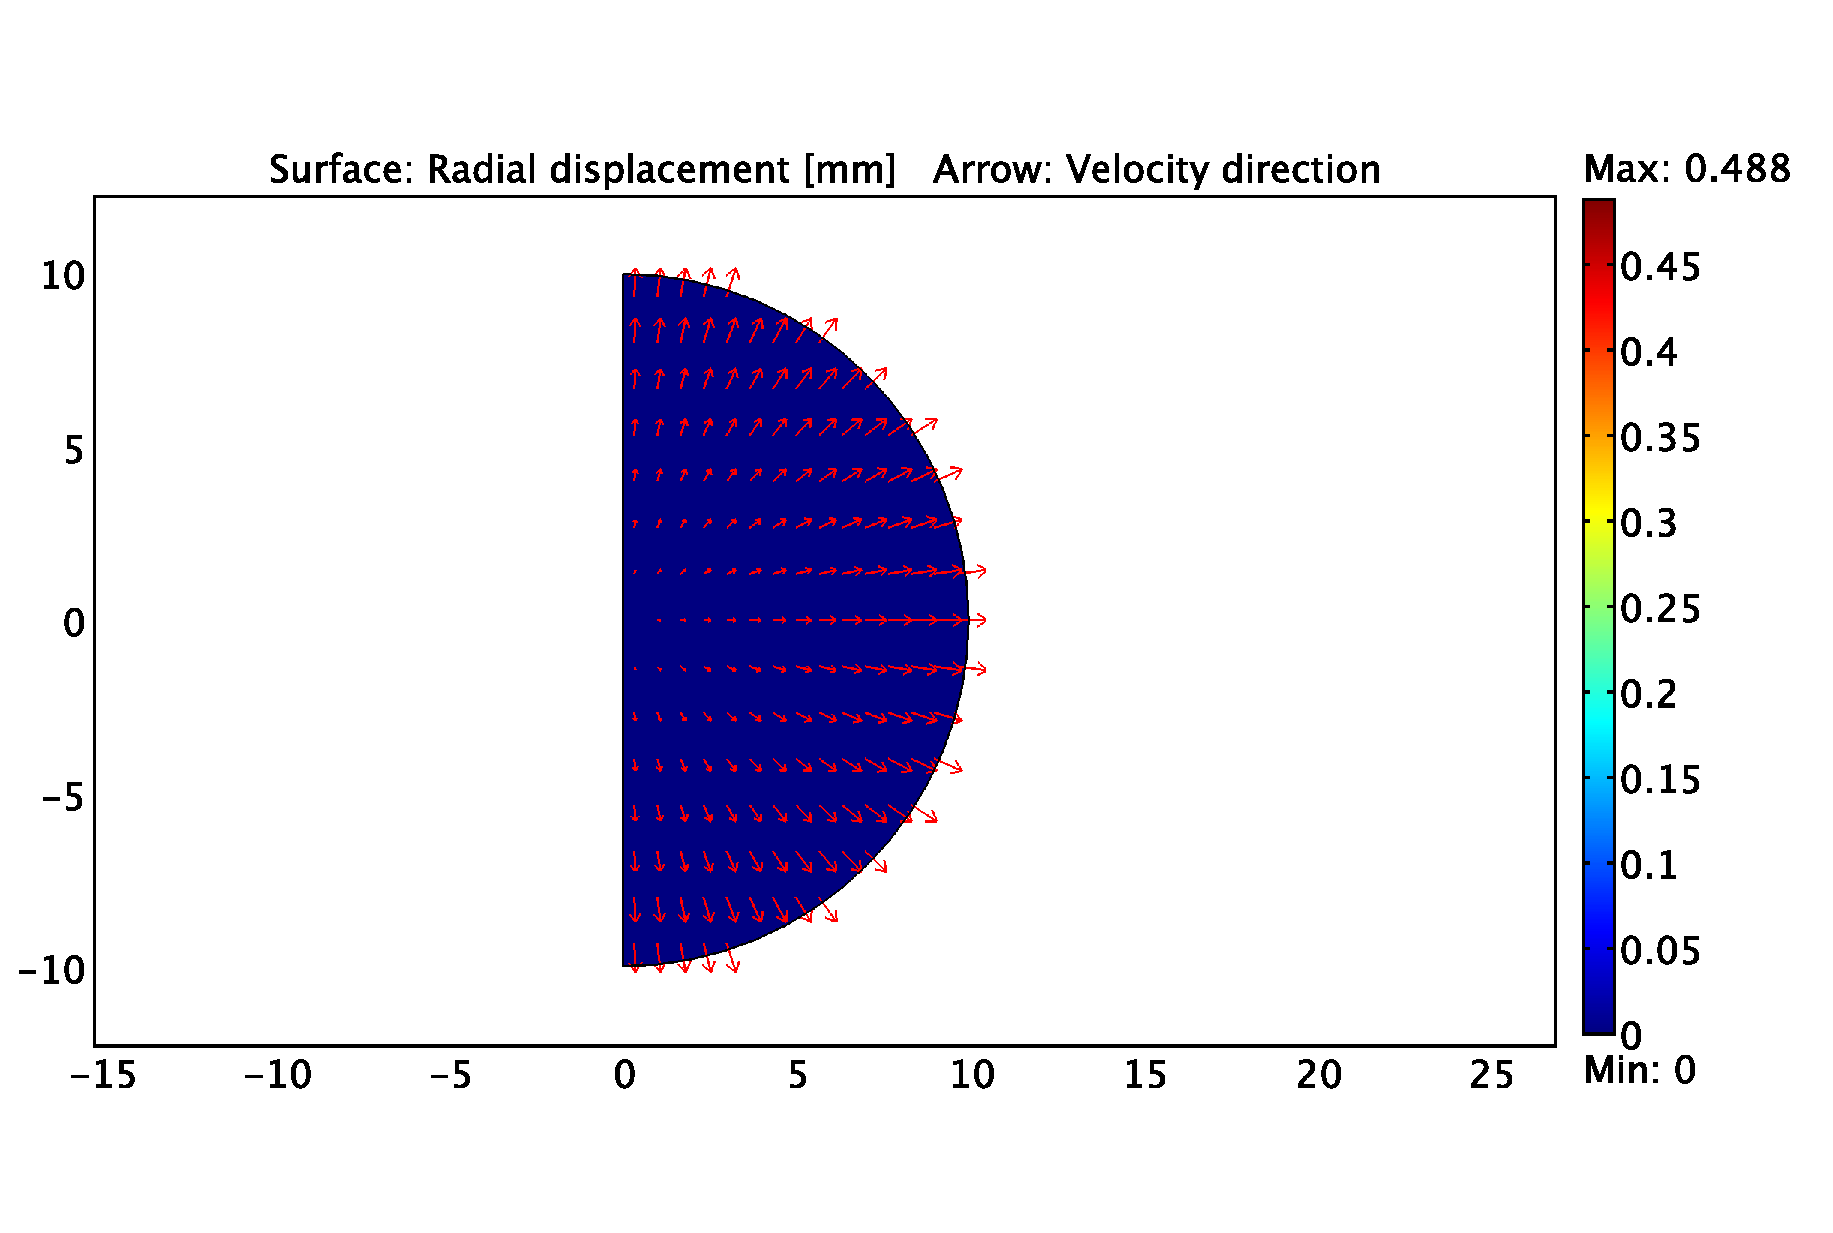
\includegraphics[width=0.9\textwidth]{images/examples/%
eulerian/cancer/isotropic-swelling-0}
\caption{A semicircular tumour at time $t=0$ days.}
\label{tumour-isotropic-swelling-0}
\end{figure}

\begin{figure}[!hptb]
\centering
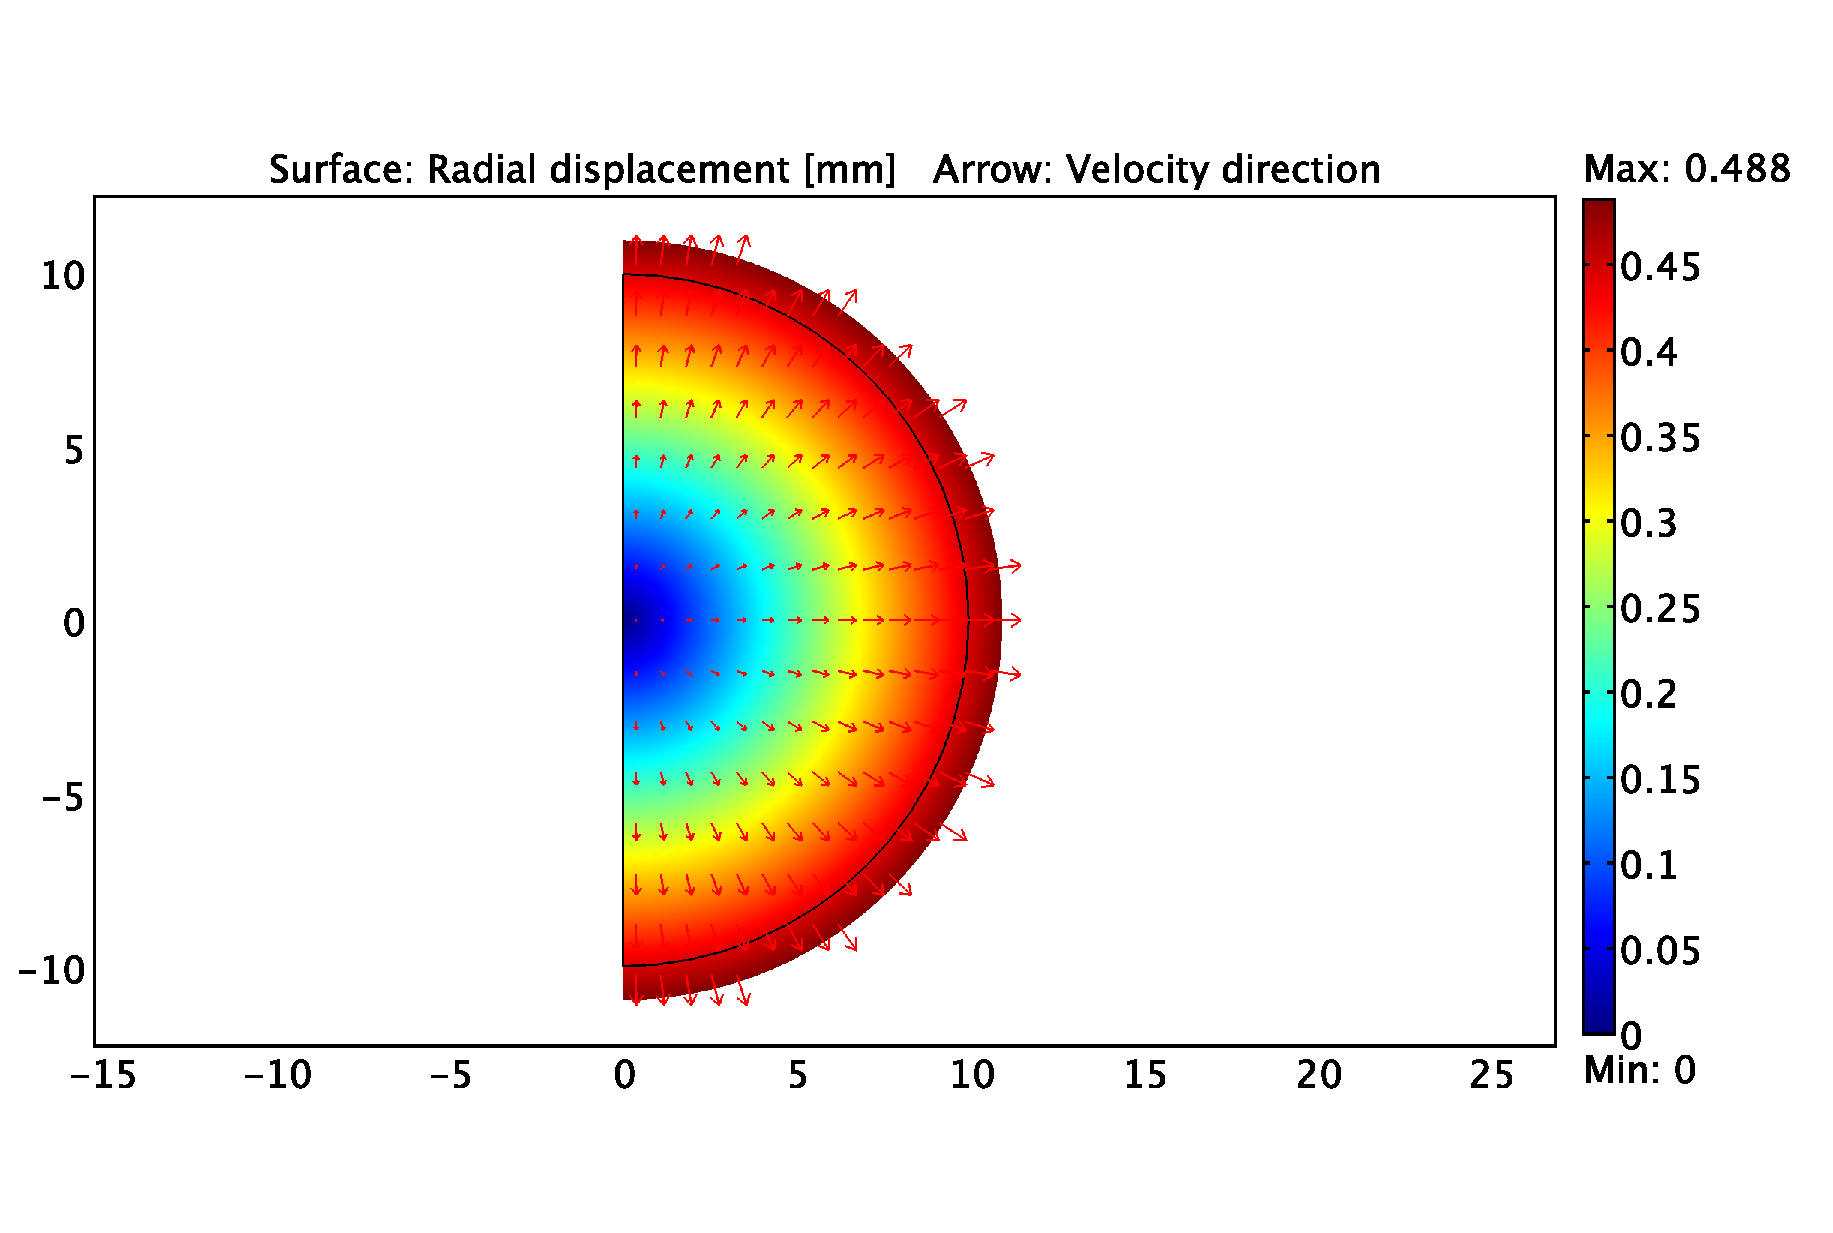
\includegraphics[width=0.9\textwidth]{images/examples/%
eulerian/cancer/isotropic-swelling-100}
\caption{A semicircular tumour at time $t=100$ days.}
\label{tumour-isotropic-swelling-100}
\end{figure}

\begin{figure}[!hptb]
\centering
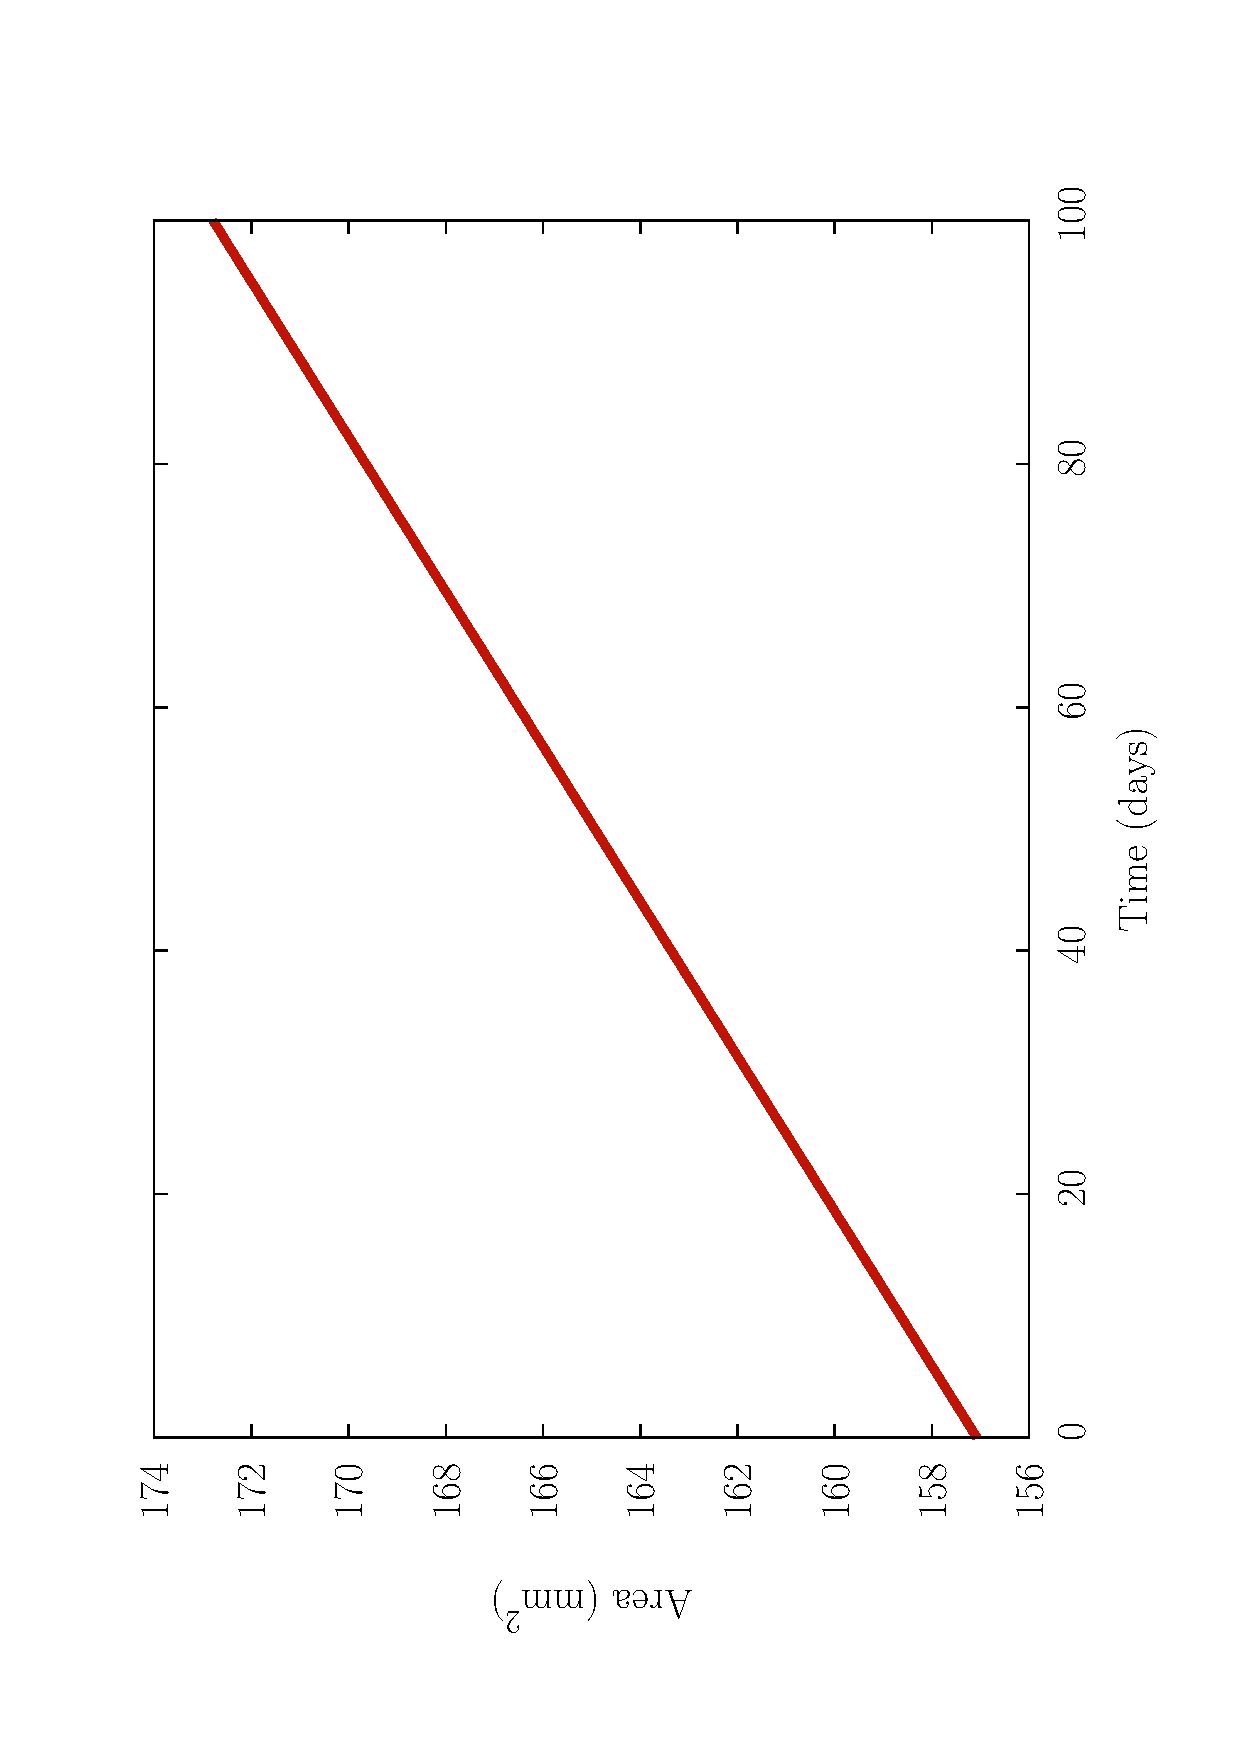
\includegraphics[width=0.6\textwidth,angle=270]{images/examples/%
eulerian/cancer/isotropic-swelling-area-evolution}
\caption{The area of the tumour evolving over 100 days.}
\label{tumour-isotropic-area-evolution}
\end{figure}

\subsection{A constraining wall and soft contact mechanics}
\label{wall-constraint}

We are interested in subjecting this solid tumour model to a
compressive stress, and the way we go about imposing this is to
introduce a rigid wall 10.5~mm to the right of the vertical edge
of the domain, and allowing the swelling tumour to impinge upon
it. Recall that the initial radius of the semicircular domain is
10~mm, thus giving it 0.5~mm to grow before it contacts the wall.

For this calculation, the solid is assumed to be hyperelastic with the
Mooney-Rivlin strain energy function~(\ref{mooney-rivlin-model}) with
constants $C_{10}=0.37$ and $C_{10}=0.11$ MPa. As in the previous
calculation, the balance of mass and momentum for this growing solid
are solved in the reference configuration. Since we are solving the
momentum balance with dynamics, we cannot introduce the rigid wall
instantaneously as this results in time-discontinuous solid velocity
fields. We instead use the following ``soft'' contact mechanics model,

\begin{equation}
q = - A \exp (-B g),
\end{equation}

\noindent where $q$ is the horizontal traction force induced by the
wall, $g$ is the gap between the wall and the approaching tumour, and
$A$ and $B$ are parameters associated with the contact model that
control the magnitude of the force, and how sharply the force rises as
the tumour approaches the wall. This model ensures that the velocity
fields on the impinging boundary of the tumour remain smooth in time.

Starting with the same initial conditions as the previous test
(Figure~\ref{tumour-isotropic-swelling-0}),
Figure~\ref{tumour-constrained-swelling-120} depicts the compressive
horizontal stress built up in the solid after 120~days due to the
presence of the wall (not visible in the figure). Notice that the
velocity vectors are much smaller in the constrained
direction. Figure~\ref{tumour-constrained-stress-evolution} shows the 
time evolution of the compressive horizontal stress at a point near
the extreme right of the domain. The stress increases sharply as the
point gets close to the wall, but remains smooth in time.

\begin{figure}[!hptb]
\centering
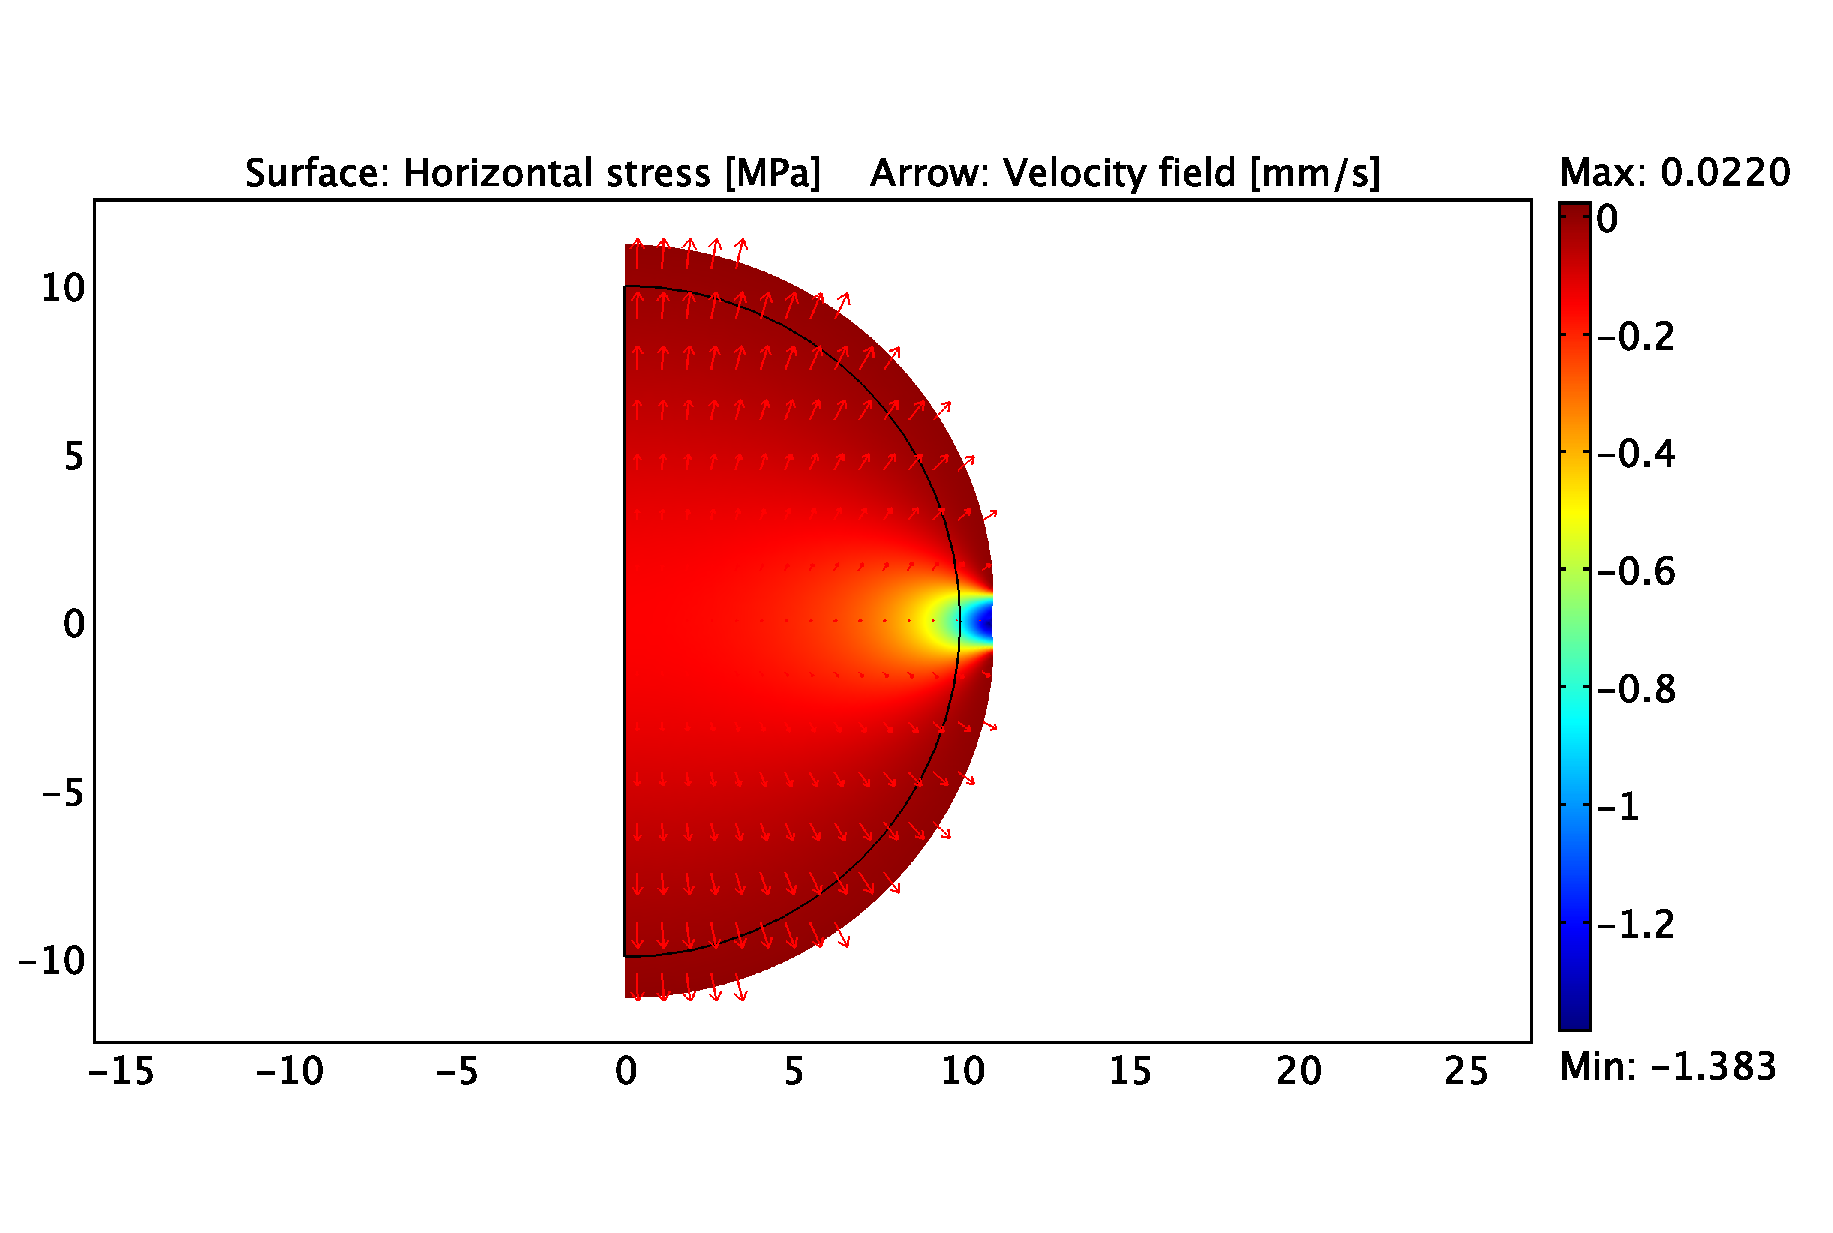
\includegraphics[width=0.9\textwidth]{images/examples/%
eulerian/cancer/constrained-swelling-120}
\caption{The growing tumour constrained by a wall at time $t=120$ days.}
\label{tumour-constrained-swelling-120}
\end{figure}

\begin{figure}[!hptb]
\centering
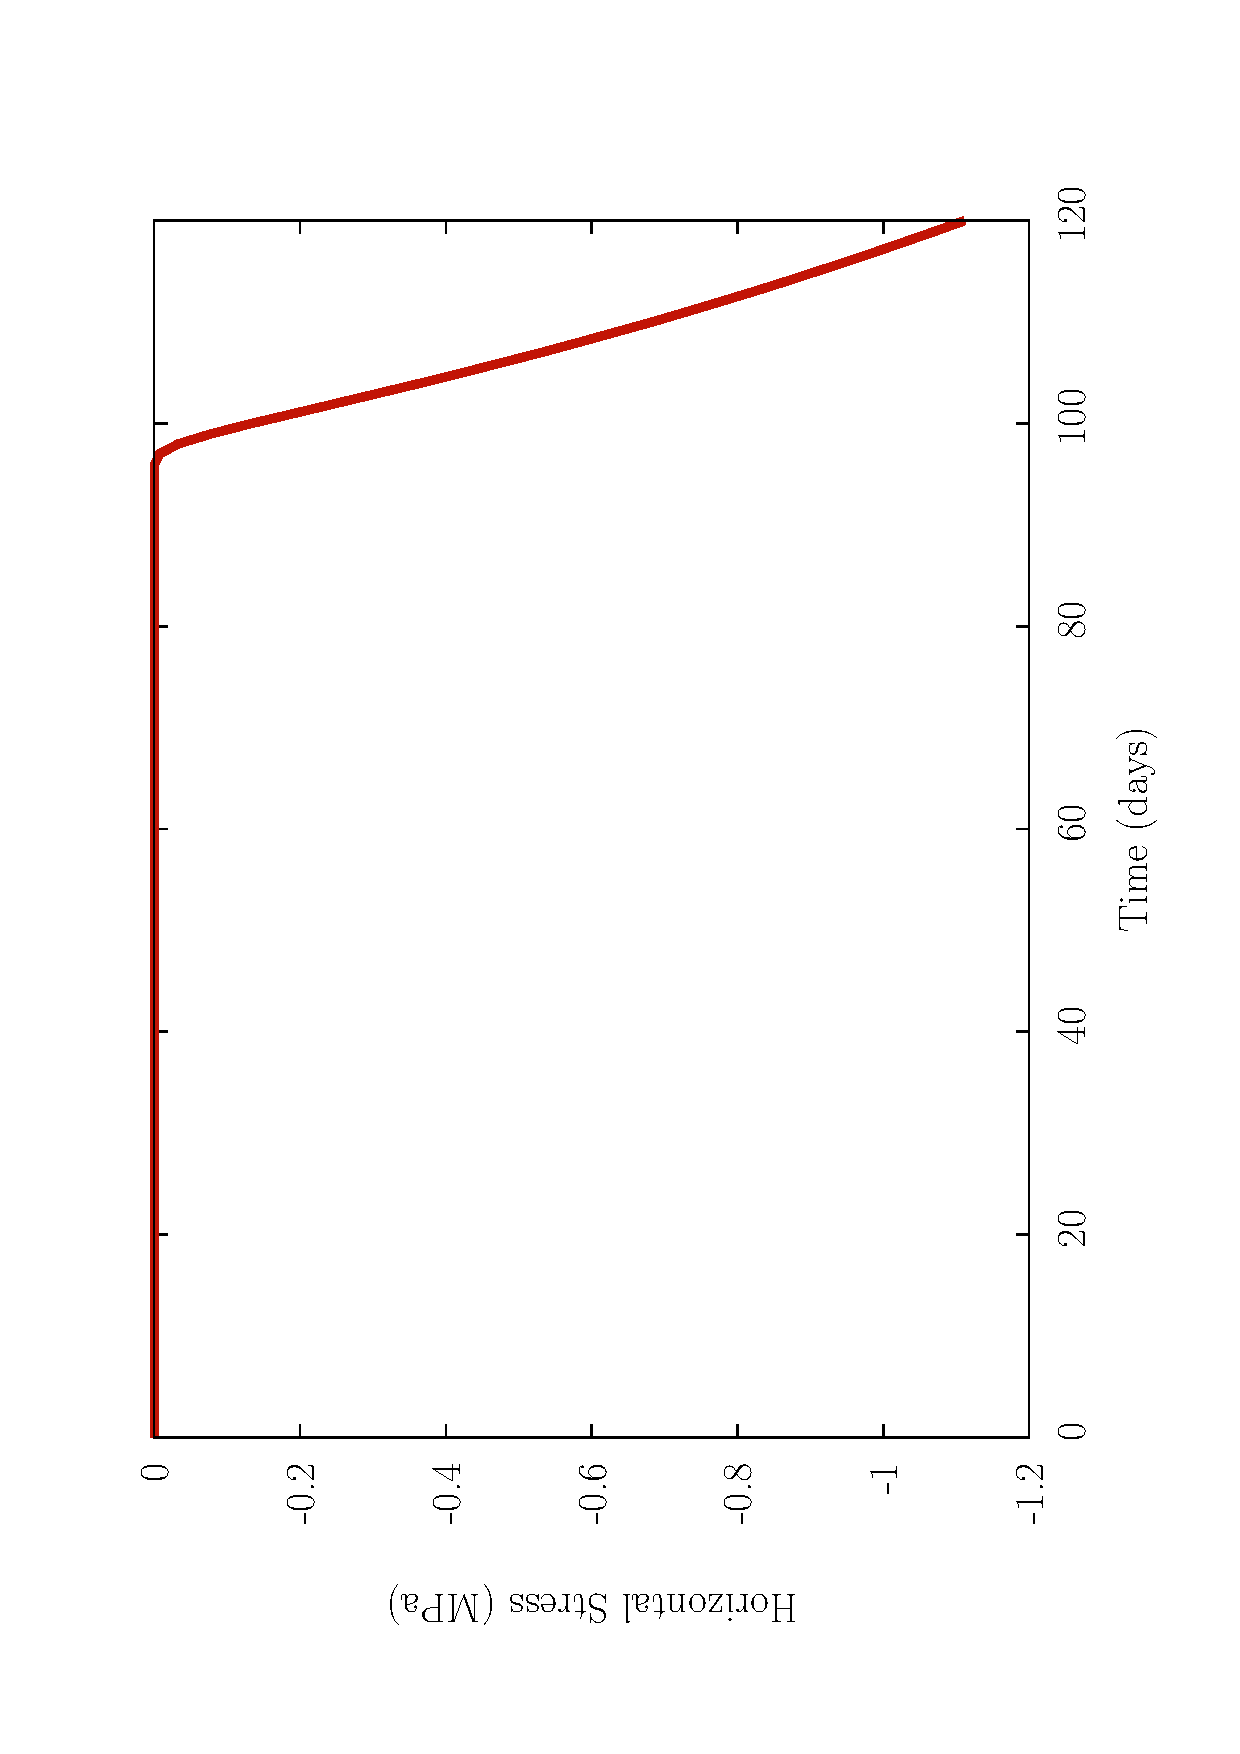
\includegraphics[width=0.6\textwidth,angle=270]{images/examples/%
eulerian/cancer/constrained-stress-evolution}
\caption{The horizontal stress in the tumour evolving over 120 days.}
\label{tumour-constrained-stress-evolution}
\end{figure}

\clearpage

\subsection{The mechanics of cells}
\label{cell-roles}

In order to observe just the gross kinematic swelling associated with
an increase in the mass of the tumour, we have treated the tumour thus
far as a homogenous solid, not distinguishing between the cells and
the ECM. In this section, we turn off the growth process, and begin to
differentiate between the species by decomposing the total solid
stress into two parts: a ``passive'' stress associated with the
hyperelastic response of the ECM, and an ``active'' stress, associated
with the cell traction forces on the surrounding medium:

\begin{equation}
\Bsigma^{\mathrm{c}} =
\underbrace{\frac{1}{J}\ \frac{\rho_{0}^{\mathrm{c}}}
  {\tilde{\rho_{0}^{\mathrm{c}}}}\    
\frac{\partial \hat{\psi^{\mathrm{c}}}}{\partial
  \bF}  \bF^{\mathrm{T}} }_{\text{Passive}}
+ \underbrace{\tau\ \rho^{\mathrm{c}} \rho^{\mathrm{cell}}
(N - \rho^{\mathrm{cell}})\ \bone.
}_{\text{Active}}
\label{activepassivesplit}
\end{equation}

\noindent This decomposition, as well as other modelling choices made
in the remaining calculations, is based on the modelling work of
\citet{namyetal:04}. Here, $\tau$ is a parameter that monitors the
individual cellular traction amplitude, $\rho^{\mathrm{c}}$ and
$\rho^{\mathrm{cell}}$ are the current concentrations of the ECM and
the cells, respectively, and $N$ is a real, positive constant
($N>\rho^{\mathrm{cell}}$) that controls the cell traction inhibition
when the cell density increases. The model assumes that the active
stresses are proportional to the ECM concentration, and that there is
a critical concentration of cells at which this active stress is
maximum.

Assuming the following uniform distribution of cells and ECM,
$\rho^{\mathrm{cell}}=0.5$~kg.m$^{-3}$ and
$\rho^{\mathrm{c}}=1$~kg.m$^{-3}$, and the values for the constants
$\tau=1000$~MPa.kg$^{-3}$.m$^{9}$ and $N=1$~kg.m$^{-3}$,
Figure~\ref{tumour-homogeneous-inward-tug} shows the cells uniformly
pulling the matrix inward. The colour contours provide the radial
displacement of the ECM. A similar calculation was performed with the
non-uniform distribution of cells (ranging between 1.18~kg.m$^{-3}$
and 4.72~kg.m$^{-3}$) shown in the colour contours in
Figure~\ref{tumour-heterogeneous-inward-tug}, and the deformed domain
shows the corresponding deformation of the ECM. Notice that the
regions of higher cell concentrations pull their surrounding ECM
neighbourhoods in greater.

\begin{figure}[!hptb]
\centering
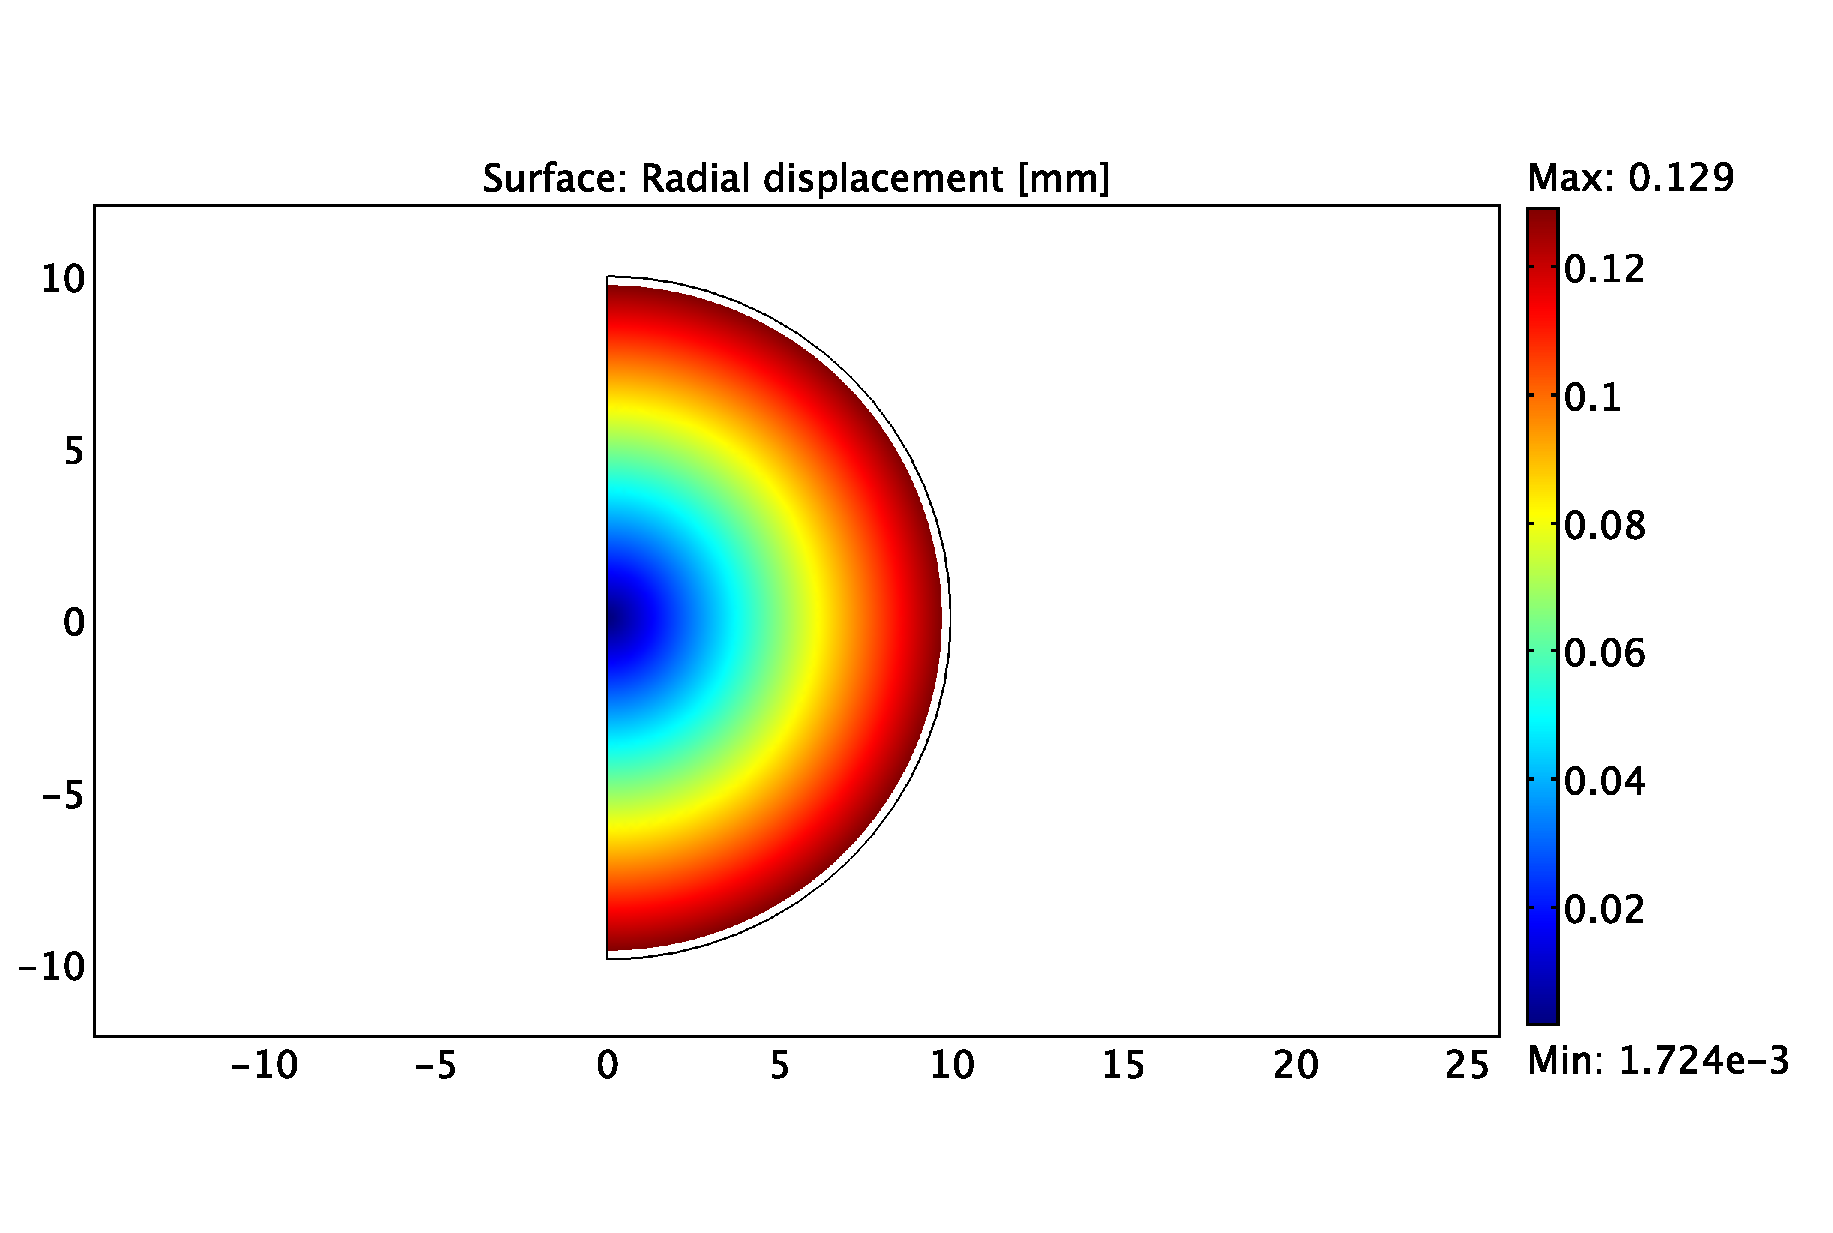
\includegraphics[width=0.9\textwidth]{images/examples/%
eulerian/cancer/homogeneous-inward-tug}
\caption{Homogeneous inward pull due to a uniform distribution of
  cells.}
\label{tumour-homogeneous-inward-tug}
\end{figure}

\begin{figure}[!hptb]
\centering
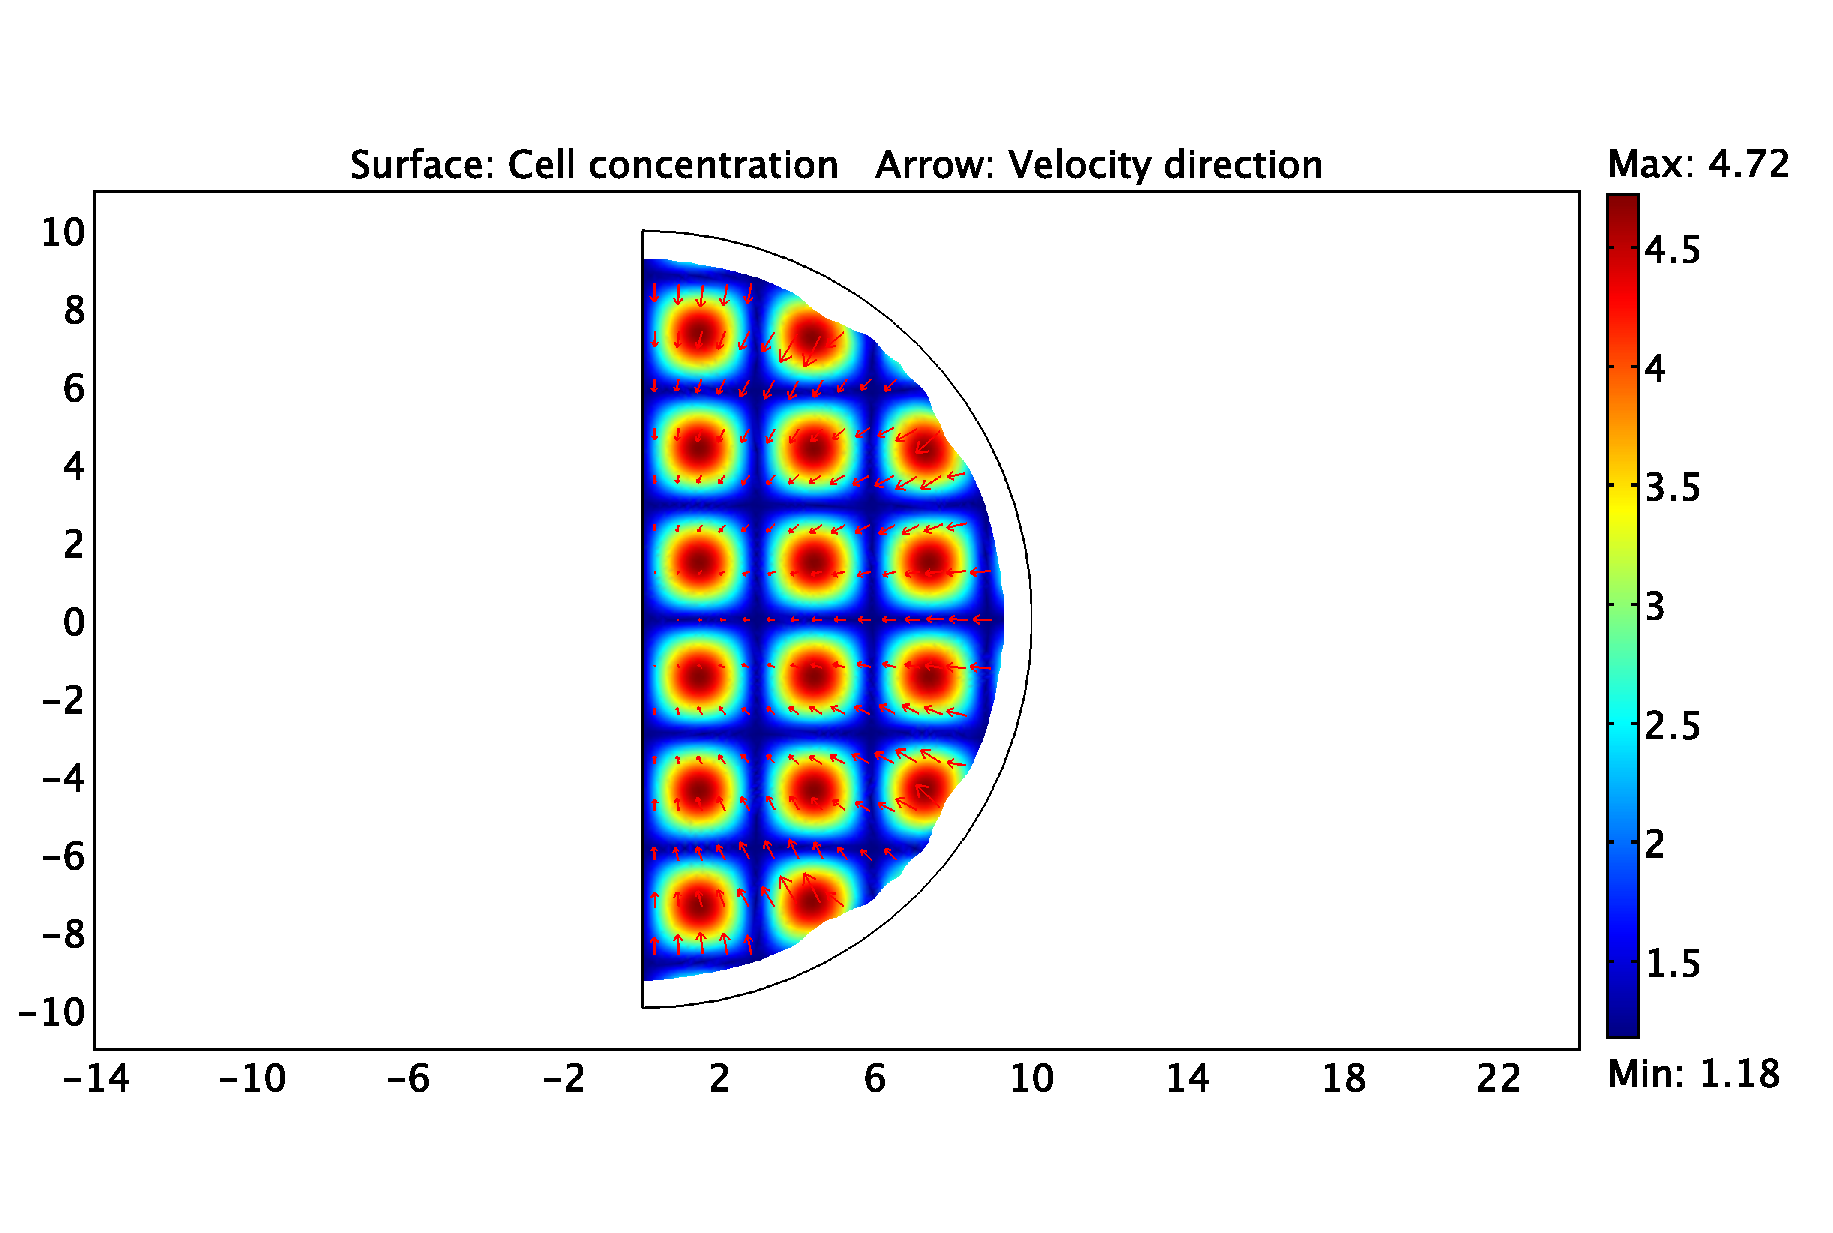
\includegraphics[width=0.9\textwidth]{images/examples/%
eulerian/cancer/heterogeneous-inward-tug}
\caption{Heterogeneous inward pull due to a non-uniform distribution
  of cells.}
\label{tumour-heterogeneous-inward-tug}
\end{figure}

\clearpage

\subsection{Transport of the cells}
\label{cell-transport}

In the calculations presented in the preceding section, the cell
concentrations were fixed spatially and temporally. In this section,
we allow for the cells to proliferate and move via diffusion and
haptotaxis (again, following the work of \citet{namyetal:04}). We
solve the mass transport equation (\ref{eu-localbalanceofmass}) for
the cells to determine their current concentration
fields. In order to account for the aforementioned modes of mass
transport, we specify the following constitutive form for the cell
mass flux:

\begin{equation}
\rho^{\mathrm{cell}}\ \bv^{\mathrm{cell}} = \underbrace{h\ \rho^{\mathrm{cell}}\
\mathrm{grad}\left(\rho^{\mathrm{c}}\right)}_{\text{Haptotactic flux}}
-\underbrace{D^{\mathrm{cell}}\ \mathrm{grad}\left(\rho^{\mathrm{cell}}\right)
}_{\text{Cell diffusion}},
\end{equation}

\noindent where $h$ is the haptotactic coefficient and
$D^{\mathrm{cell}}$ is the diffusivity of the cells in the matrix. In
this section, we are primarily interested in observing the
proliferation and transport of the cells, and so we will not associate
any kinematics with the changing concentration of cells.

In the first set of results, we look at cell proliferation and
diffusion, and observe the effect that this has on the traction that
they apply on their ECM neighbourhoods. Starting with a cell-rich
circle of radius 5~mm at the centre of the domain (having a uniform cell
concentration of 6.266~kg.m$^{-3}$), and a smaller cell concentration
(3.778~kg.m$^{-3}$) everywhere else; and using a uniform cell source
$\pi^{\mathrm{cell}}=0.001$~kg.m$^{-3}$/day and a diffusion
coefficient of $D^{\mathrm{cell}}=0.01$~mm$^2$/day,
Figures~\ref{tumour-diffusion-proliferation-0}--Figure~%
\ref{tumour-diffusion-proliferation-100} show the snapshots of the
diffusing and proliferating cells during the course of the test. The colour
contours provide the evolving cell concentration fields and the arrows
provide the deformation direction of the ECM, induced by the cell
traction.

\clearpage

\begin{figure}[!hptb]
\centering
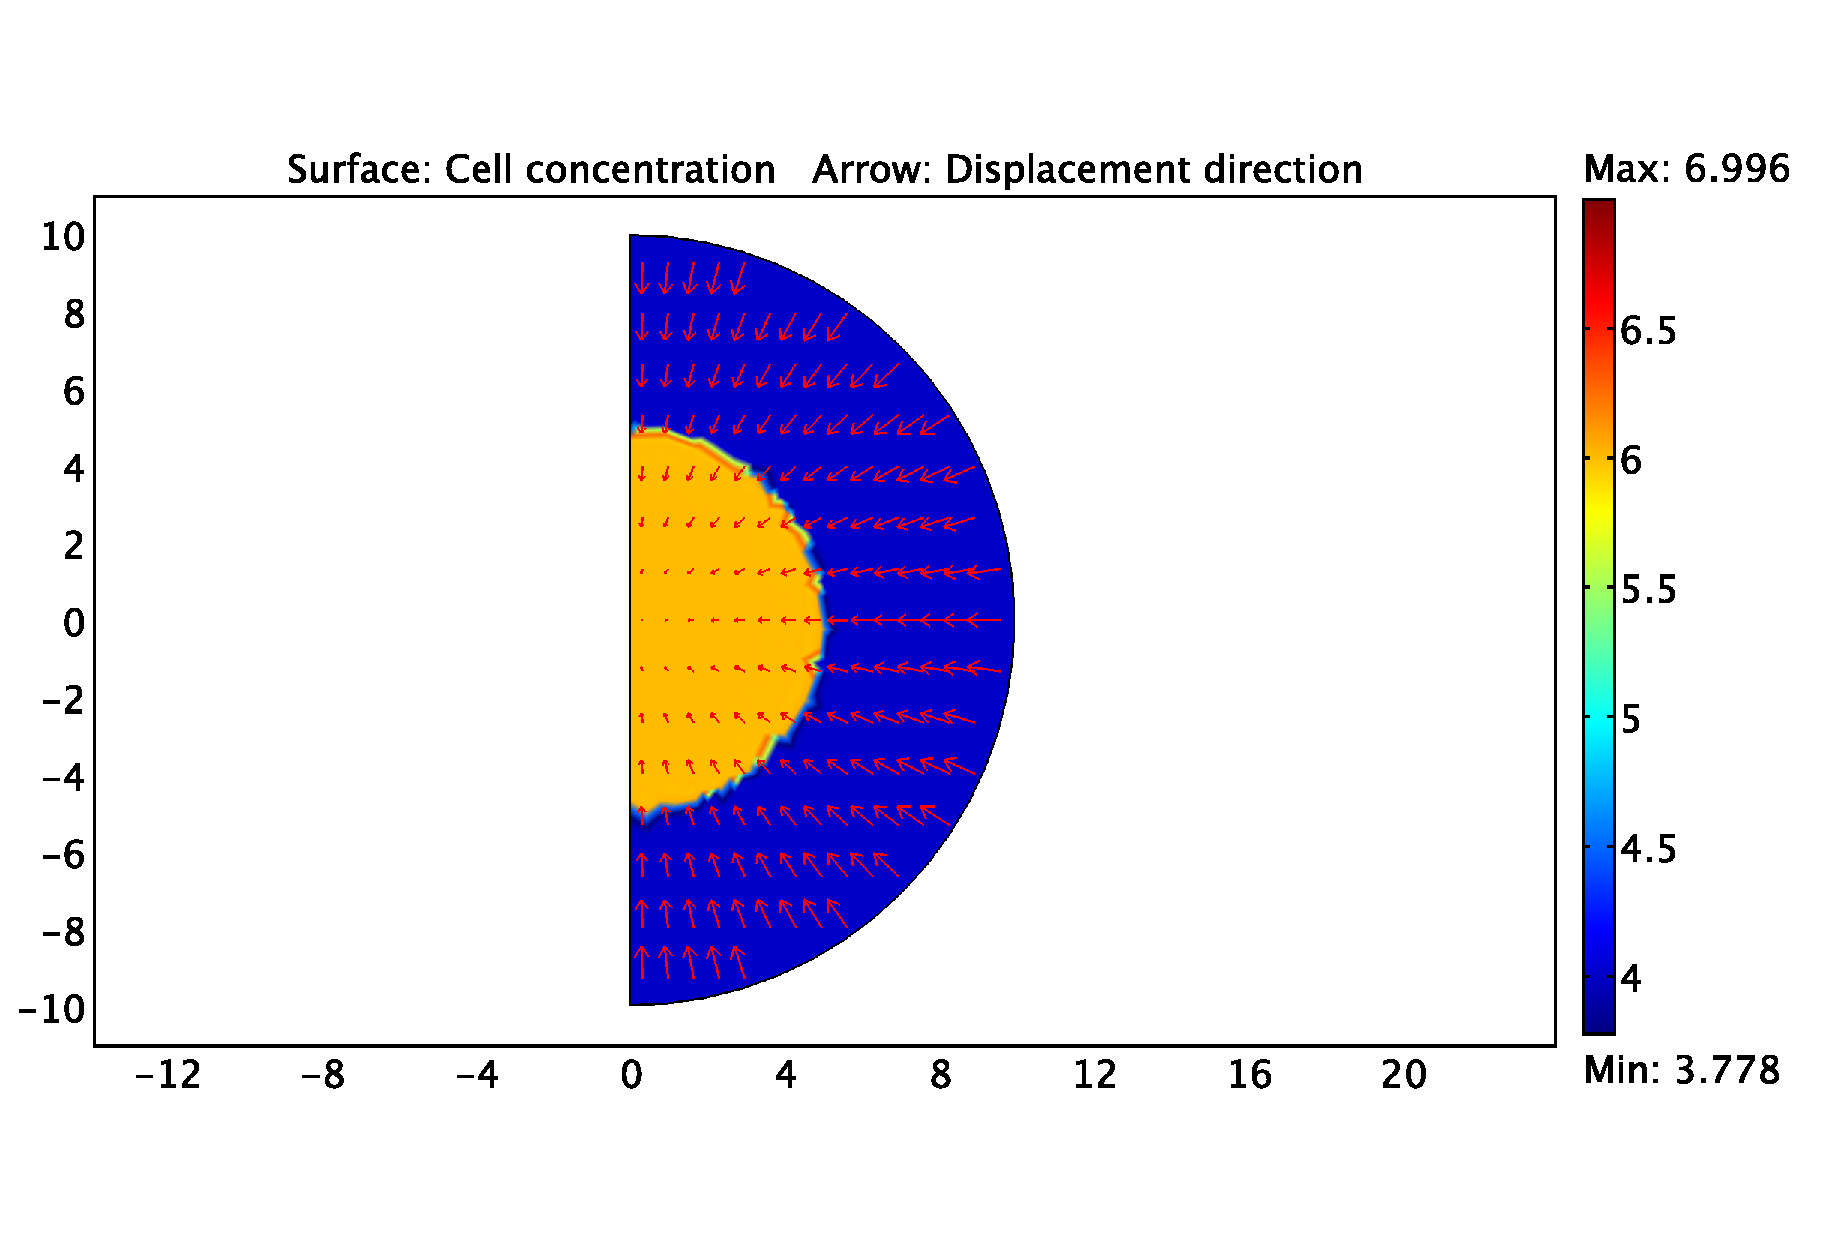
\includegraphics[width=0.9\textwidth]{images/examples/%
eulerian/cancer/diffusing-proliferating-cells-0}
\caption{The cells diffusing and proliferating at time $t=0$ days.}
\label{tumour-diffusion-proliferation-0}
\end{figure}

\begin{figure}[!hptb]
\centering
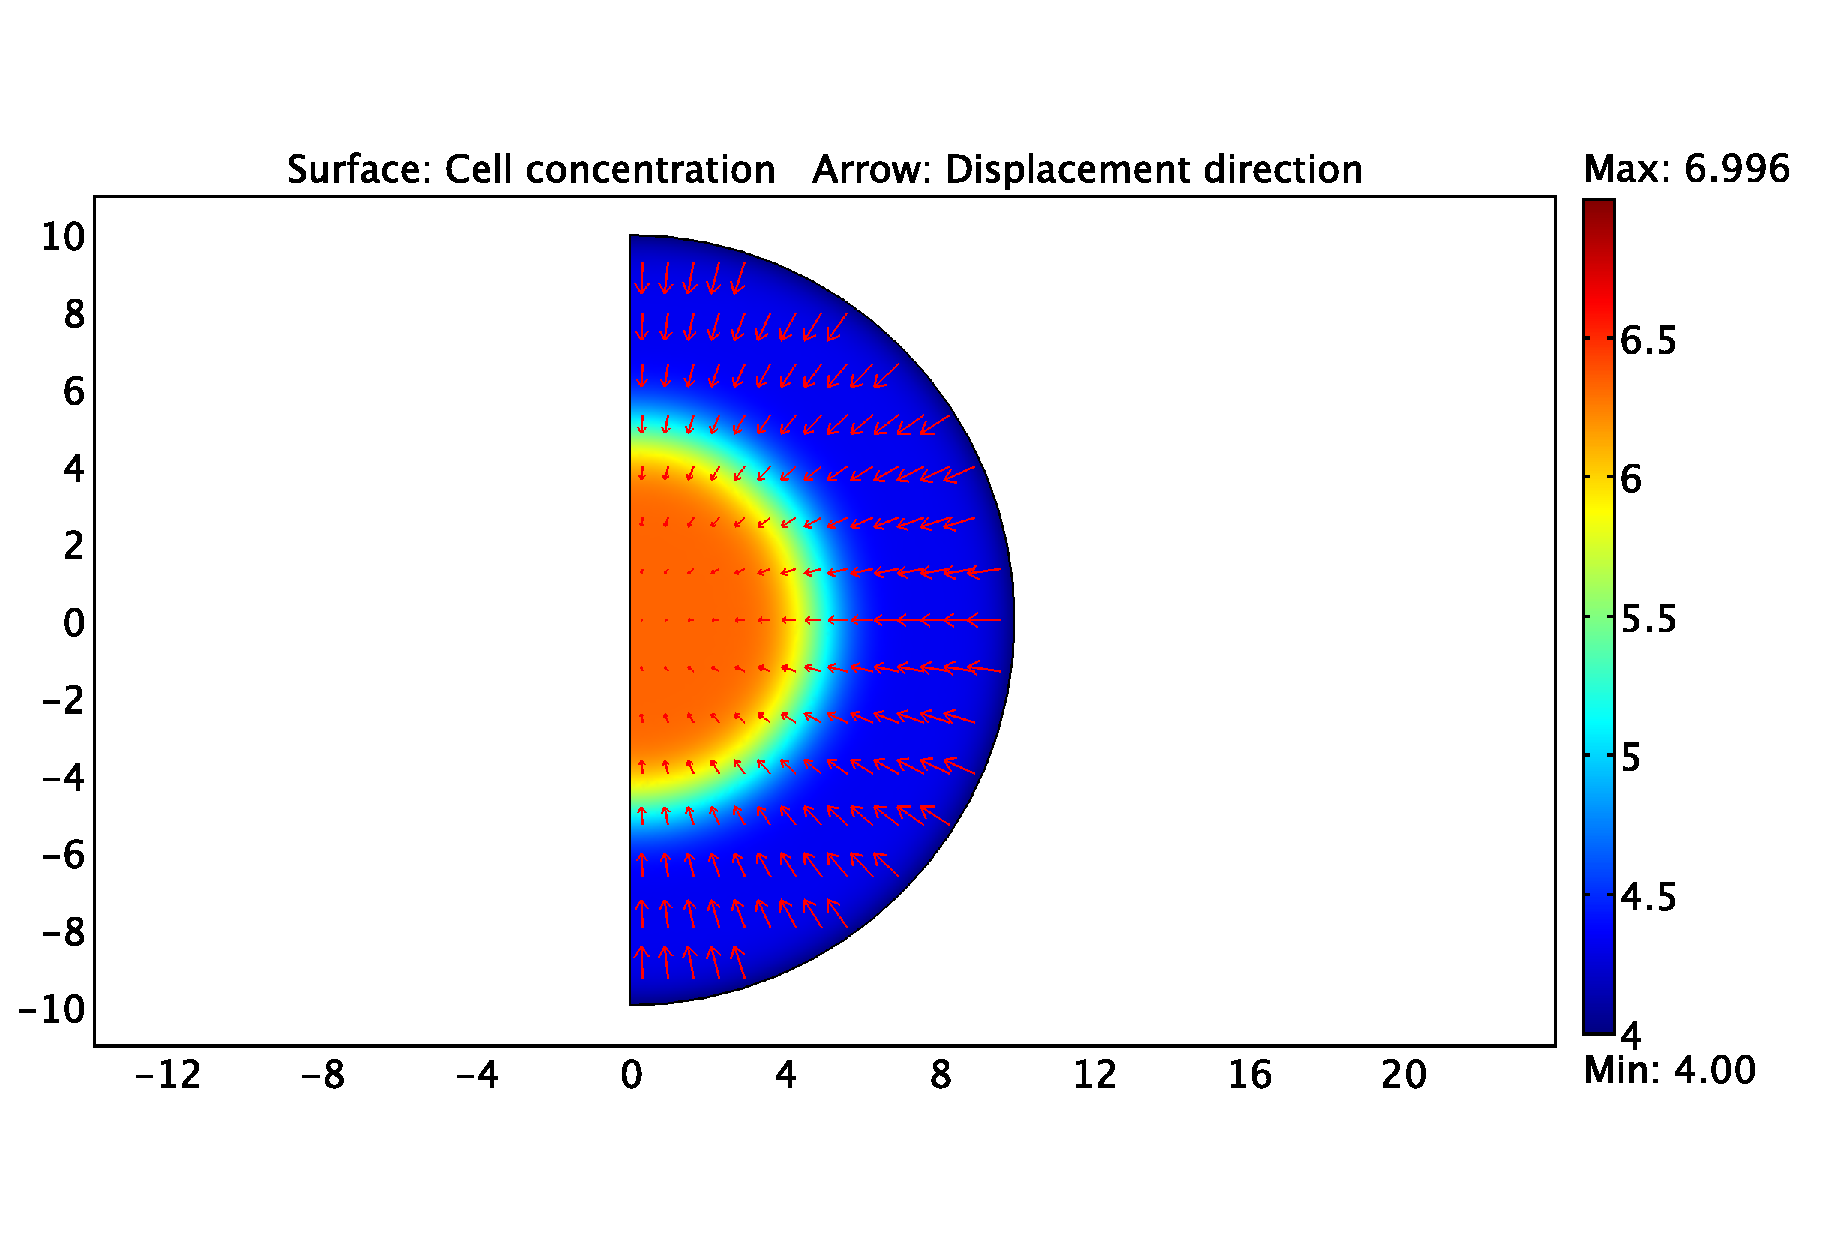
\includegraphics[width=0.9\textwidth]{images/examples/%
eulerian/cancer/diffusing-proliferating-cells-33}
\caption{The cells diffusing and proliferating at time $t=33$ days.}
\label{tumour-diffusion-proliferation-33}
\end{figure}

\begin{figure}[!hptb]
\centering
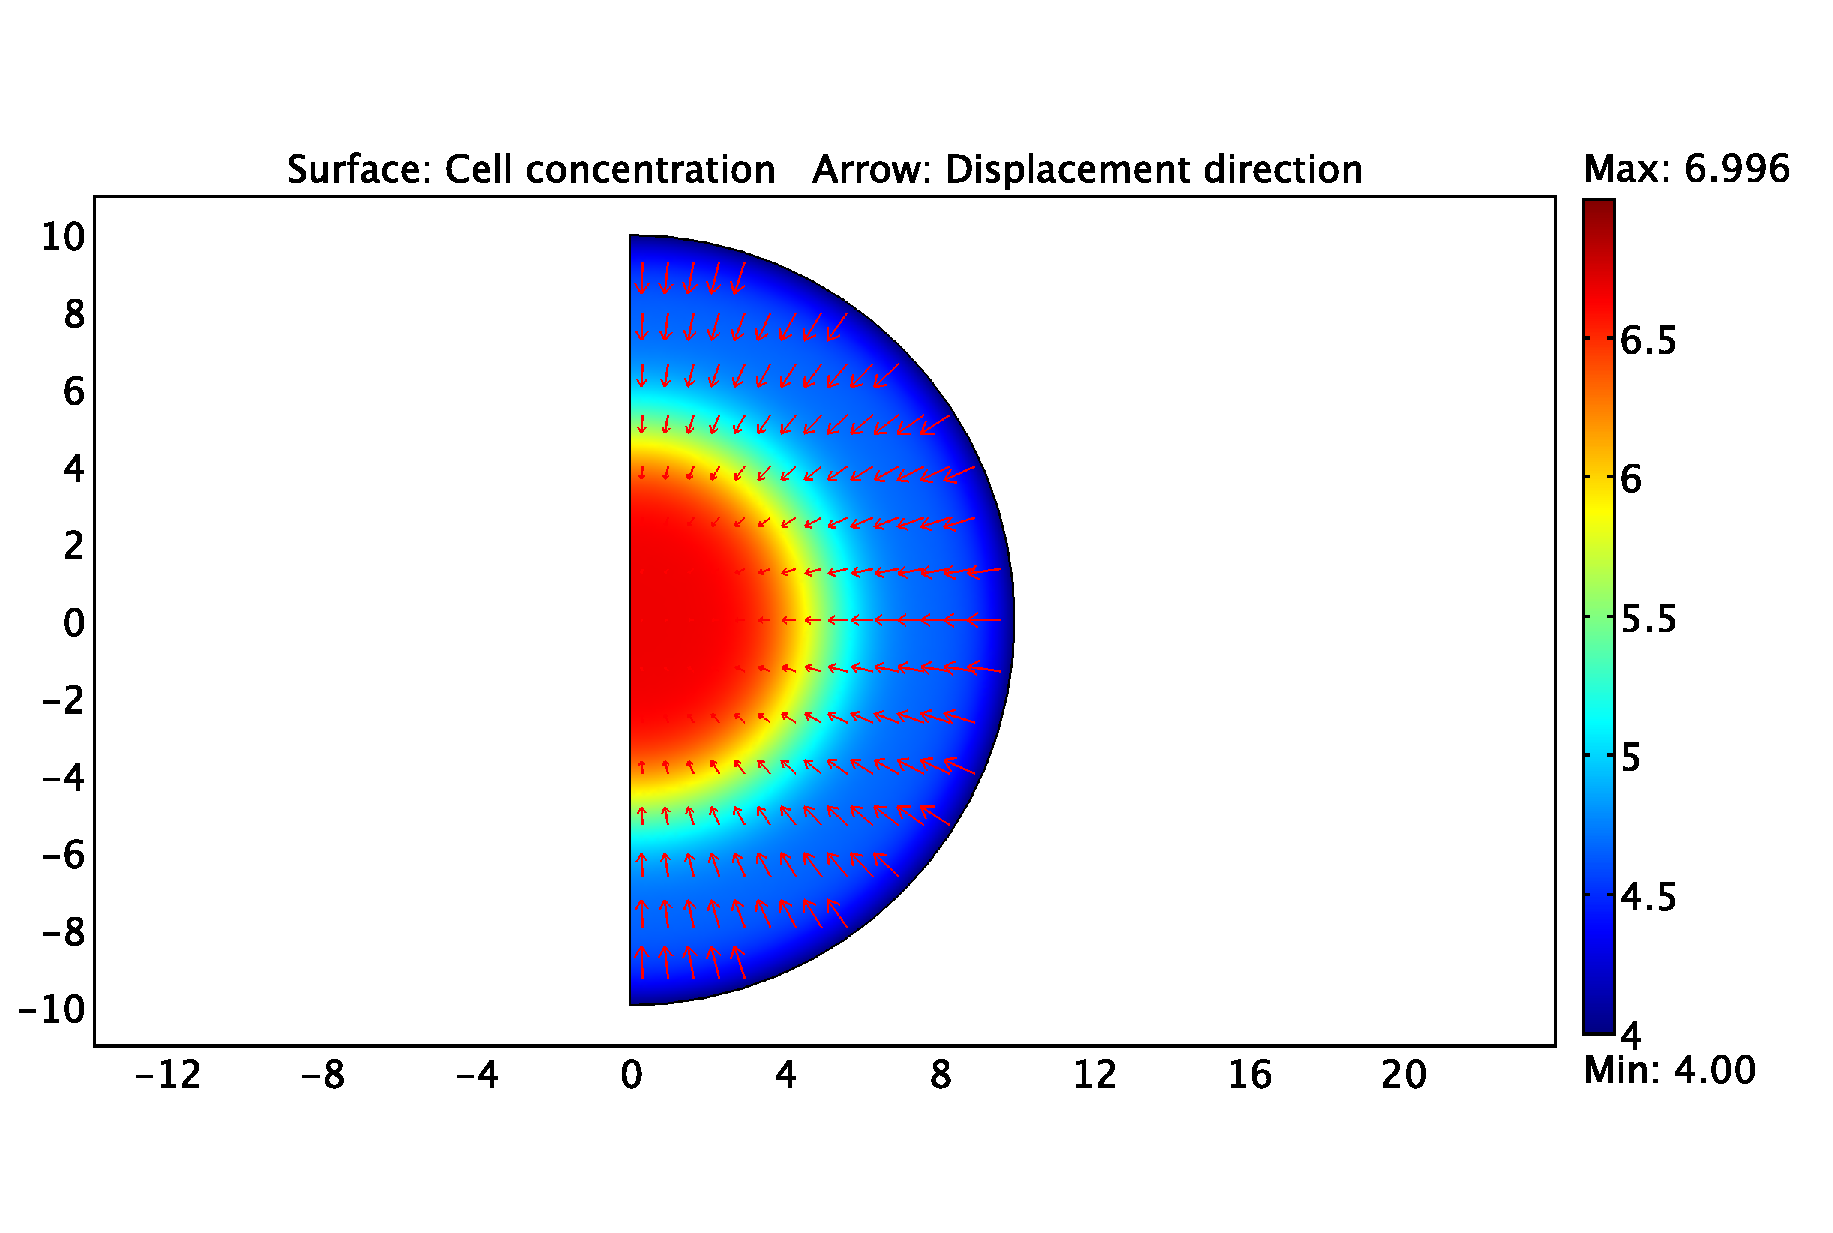
\includegraphics[width=0.9\textwidth]{images/examples/%
eulerian/cancer/diffusing-proliferating-cells-67}
\caption{The cells diffusing and proliferating at time $t=67$ days.}
\label{tumour-diffusion-proliferation-67}
\end{figure}

\begin{figure}[!hptb]
\centering
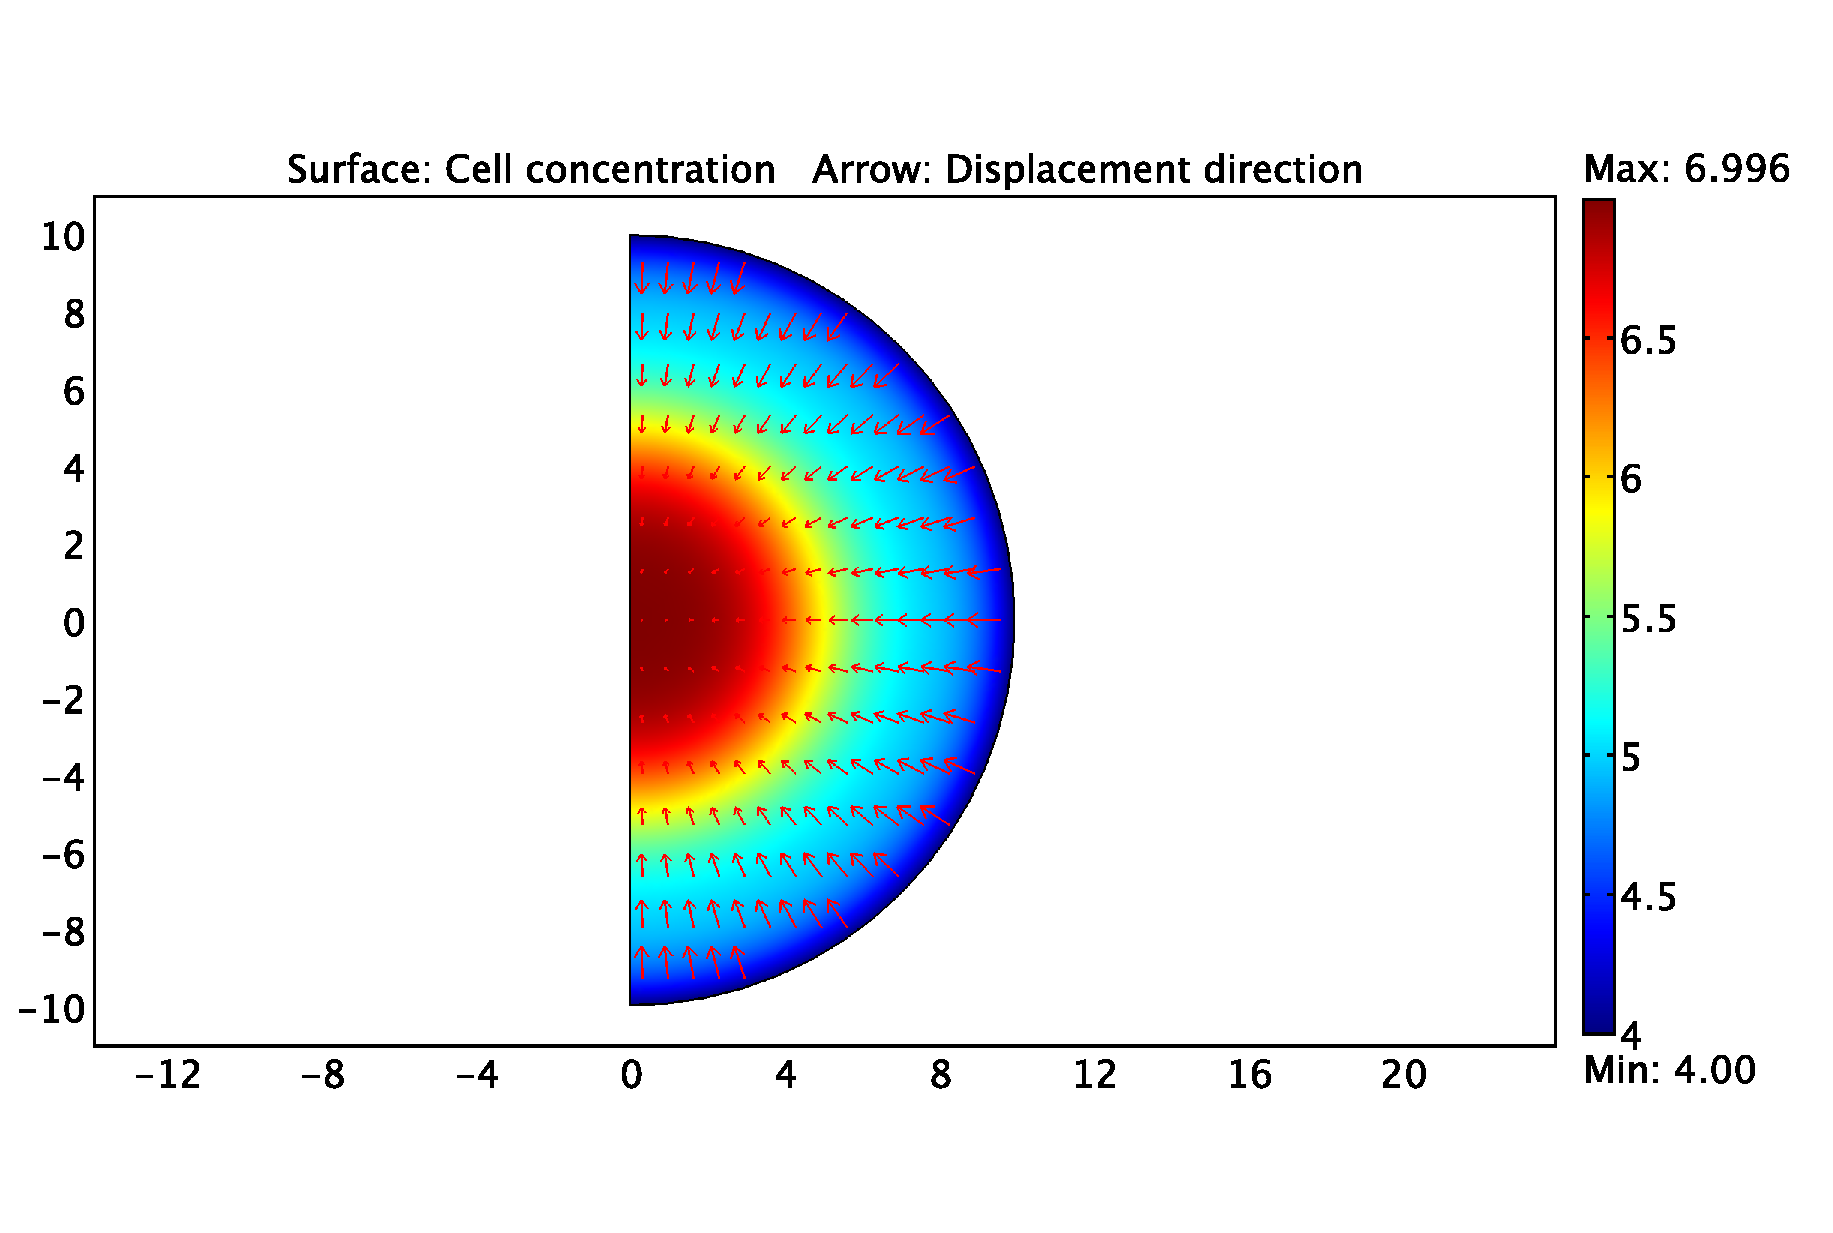
\includegraphics[width=0.9\textwidth]{images/examples/%
eulerian/cancer/diffusing-proliferating-cells-100}
\caption{The cells diffusing and proliferating at time $t=100$ days.}
\label{tumour-diffusion-proliferation-100}
\end{figure}

\clearpage

In the second set of results, we look at cell proliferation and
haptotaxis, and observe the effect that this has on the traction that
they apply on their ECM neighbourhoods. We start this test with the
same initial conditions for the cells as the previous calculation (a
cell rich bulb at the centre of the domain), but in order to induce
haptotaxis, we begin with the heterogenous ECM concentration (varying
between 0.5~kg.m$^{-3}$ and 1.5~kg.m$^{-3}$), seen in
Figure~\ref{heterogeneous-ecm-concentration}. In these tests, the
haptotactic coefficient $h$ is 0.1~mm$^2$.day$^{-1}$.mm$^3$.kg$^{-1}$.
Figures~\ref{tumour-haptotaxis-proliferation-0}--%
\ref{tumour-haptotaxis-proliferation-10} show snapshots of the cells
undergoing haptotaxis and proliferating during the course of the
test. The colour contours provide the evolving cell concentration
fields and the arrows provide the deformation direction of the ECM,
induced by the cell traction. We observe that the cells migrate toward
areas of higher ECM while proliferating. Note that the directionality
of the cell traction field changes correspondingly with the
concentration field, as noted by the lengths and directions of the
arrows.

\begin{figure}[!hptb]
\centering
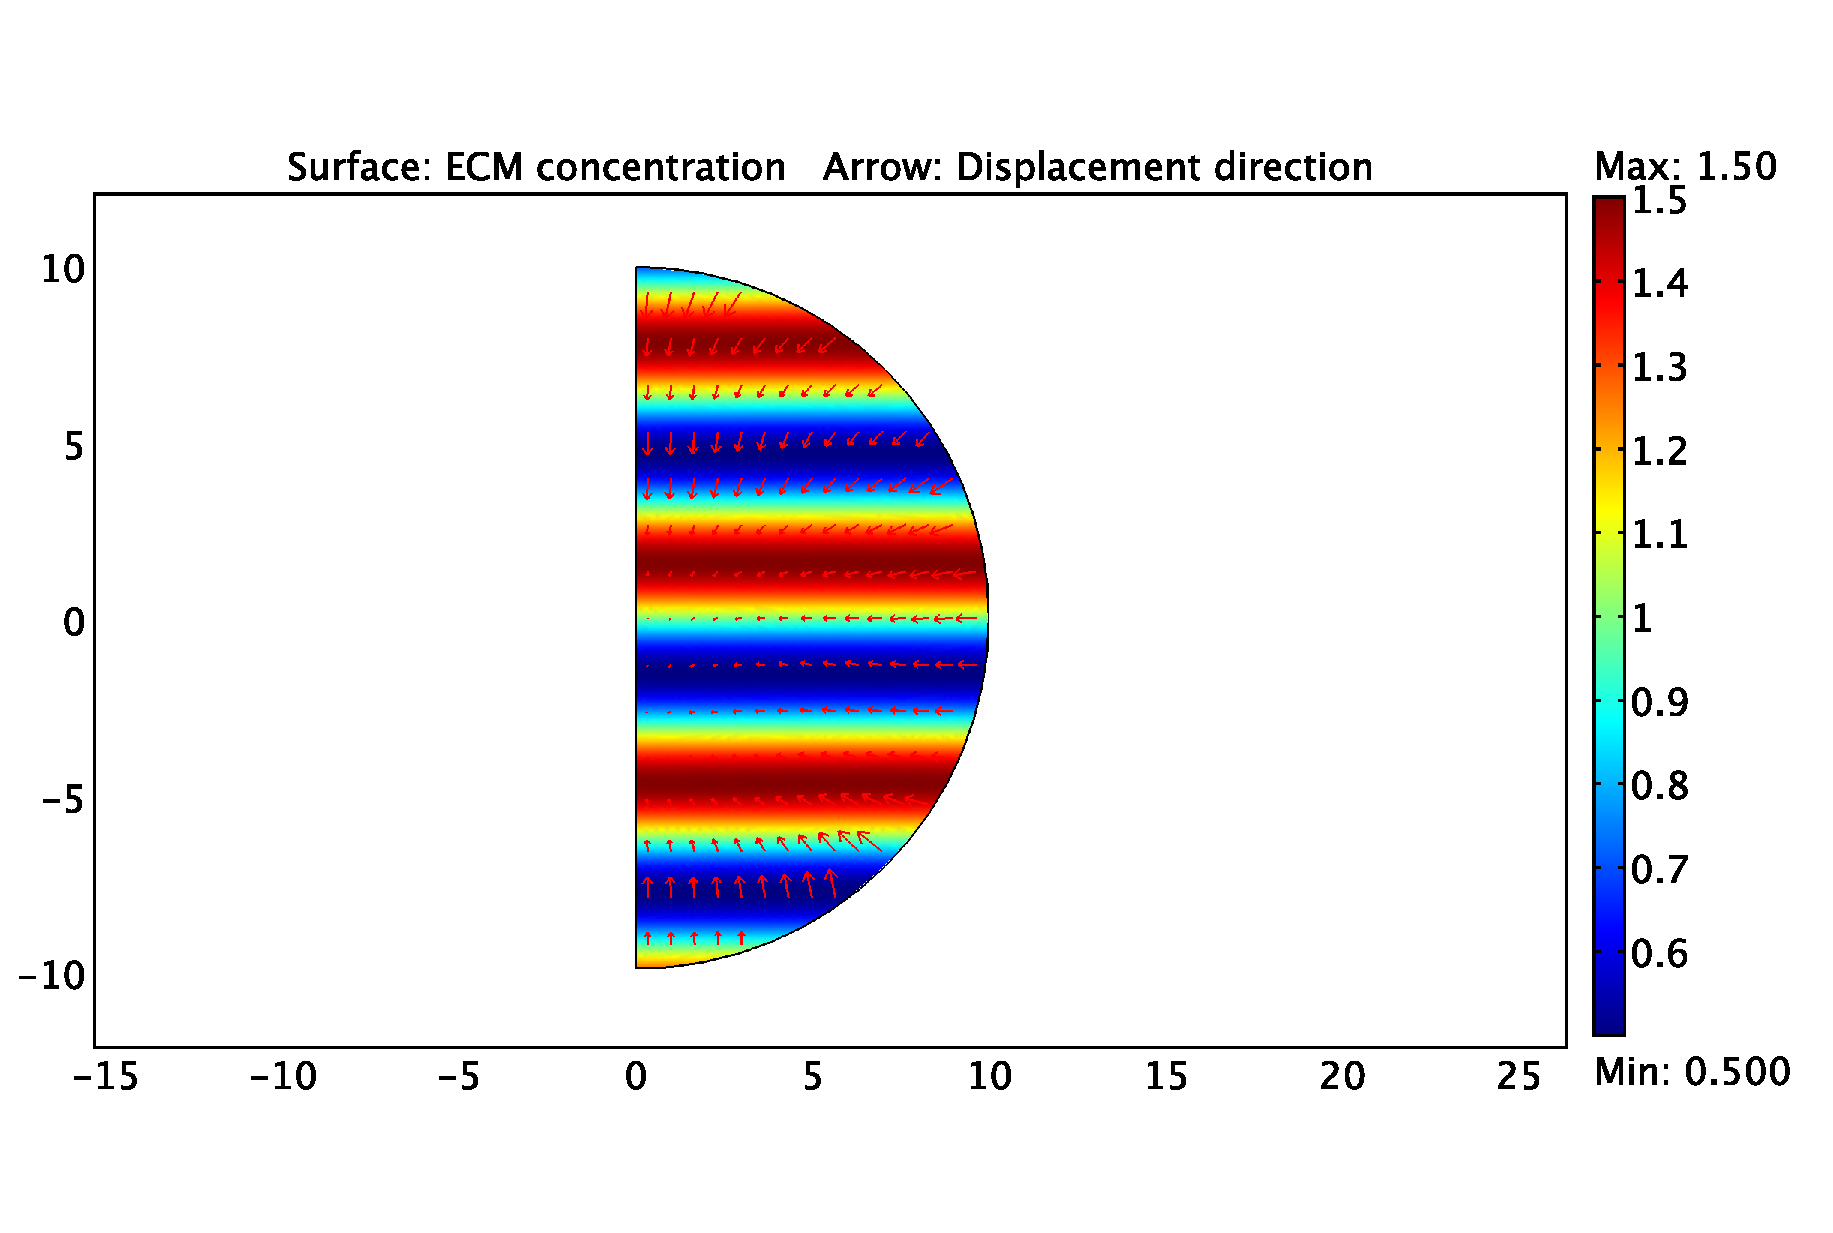
\includegraphics[width=0.9\textwidth]{images/examples/%
eulerian/cancer/heterogeneous-ecm-concentration}
\caption{Heterogeneous extra-cellular matrix concentration.}
\label{heterogeneous-ecm-concentration}
\end{figure}

\begin{figure}[!hptb]
\centering
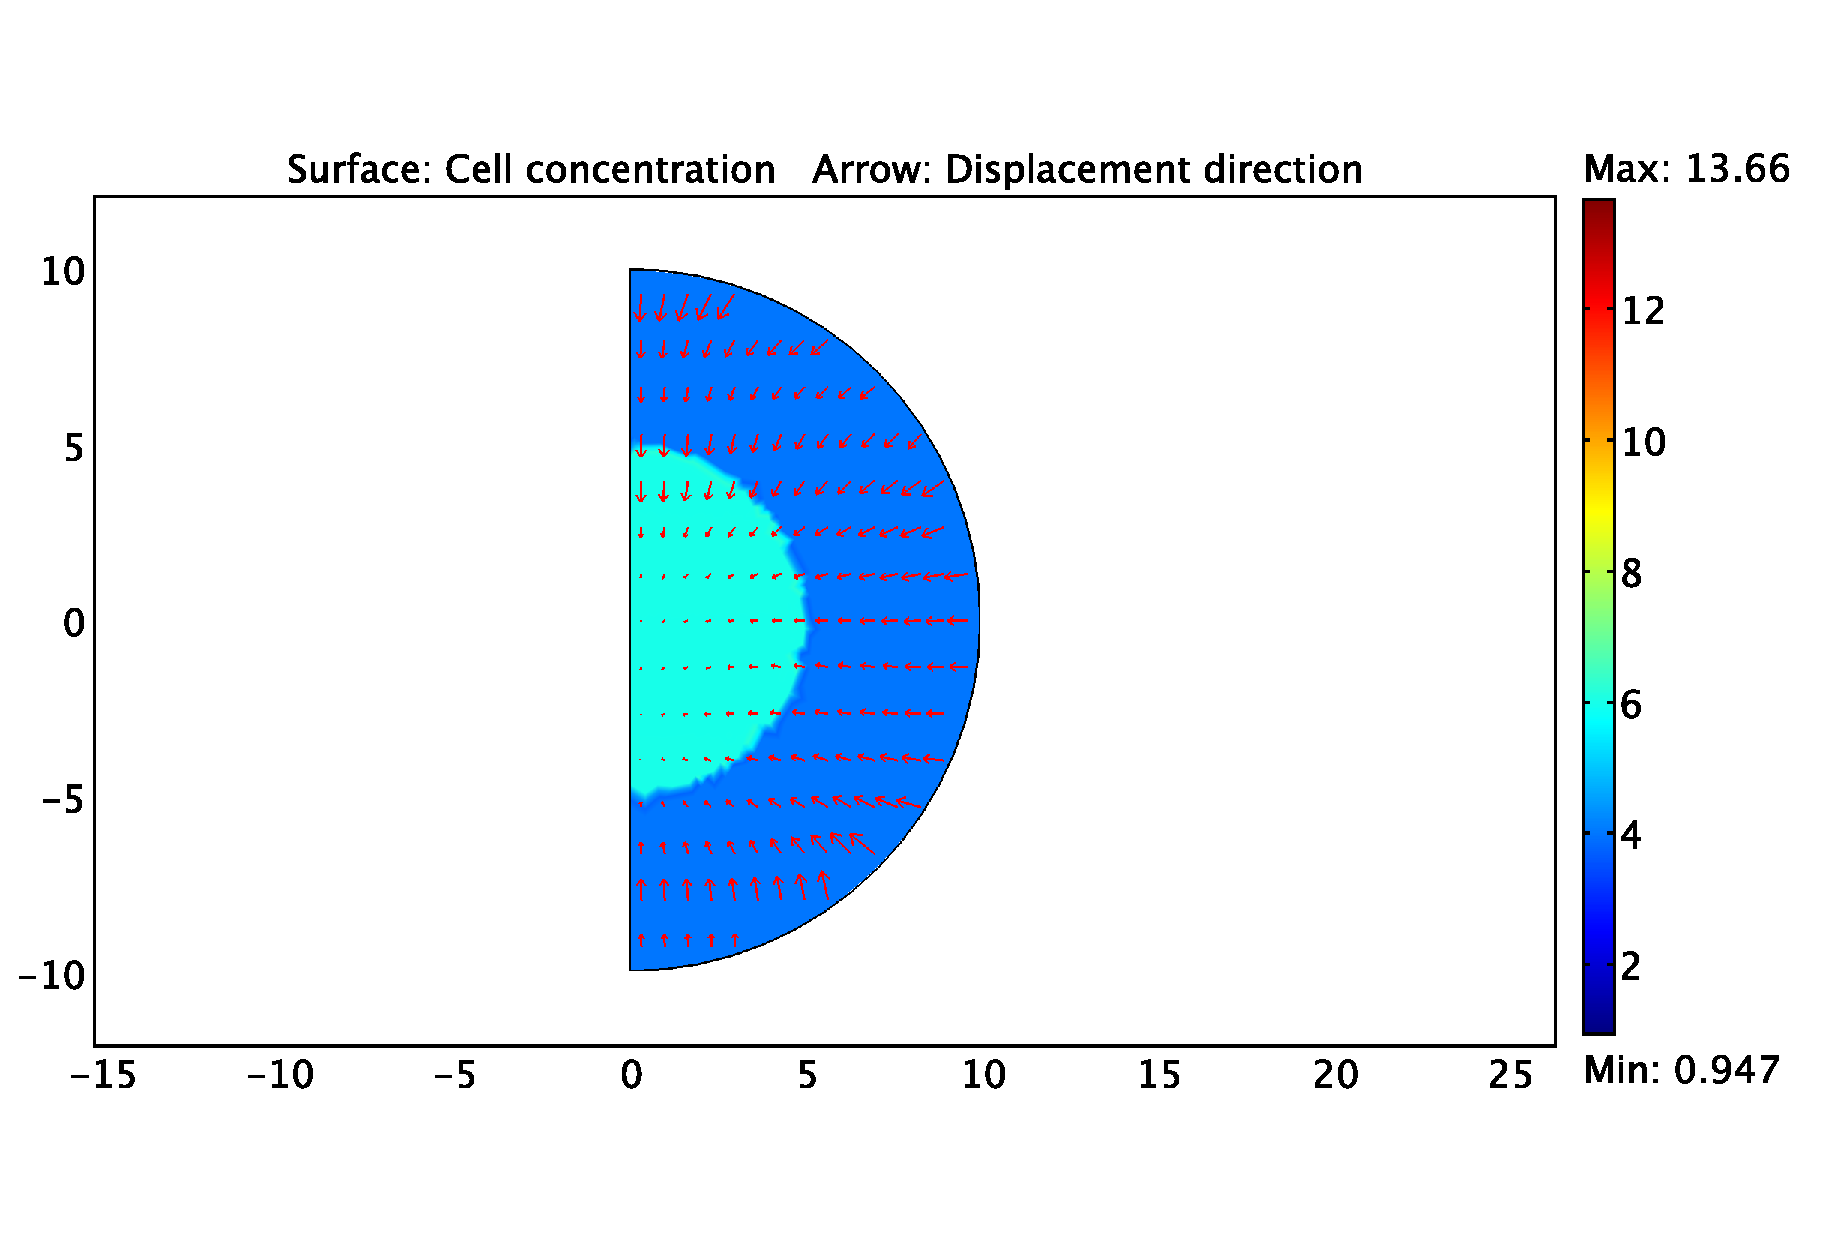
\includegraphics[width=0.9\textwidth]{images/examples/%
eulerian/cancer/haptotaxis-proliferating-cells-0}
\caption{Proliferating cells undergoing diffusion and haptotaxis at time $t=0$ days.}
\label{tumour-haptotaxis-proliferation-0}
\end{figure}

\begin{figure}[!hptb]
\centering
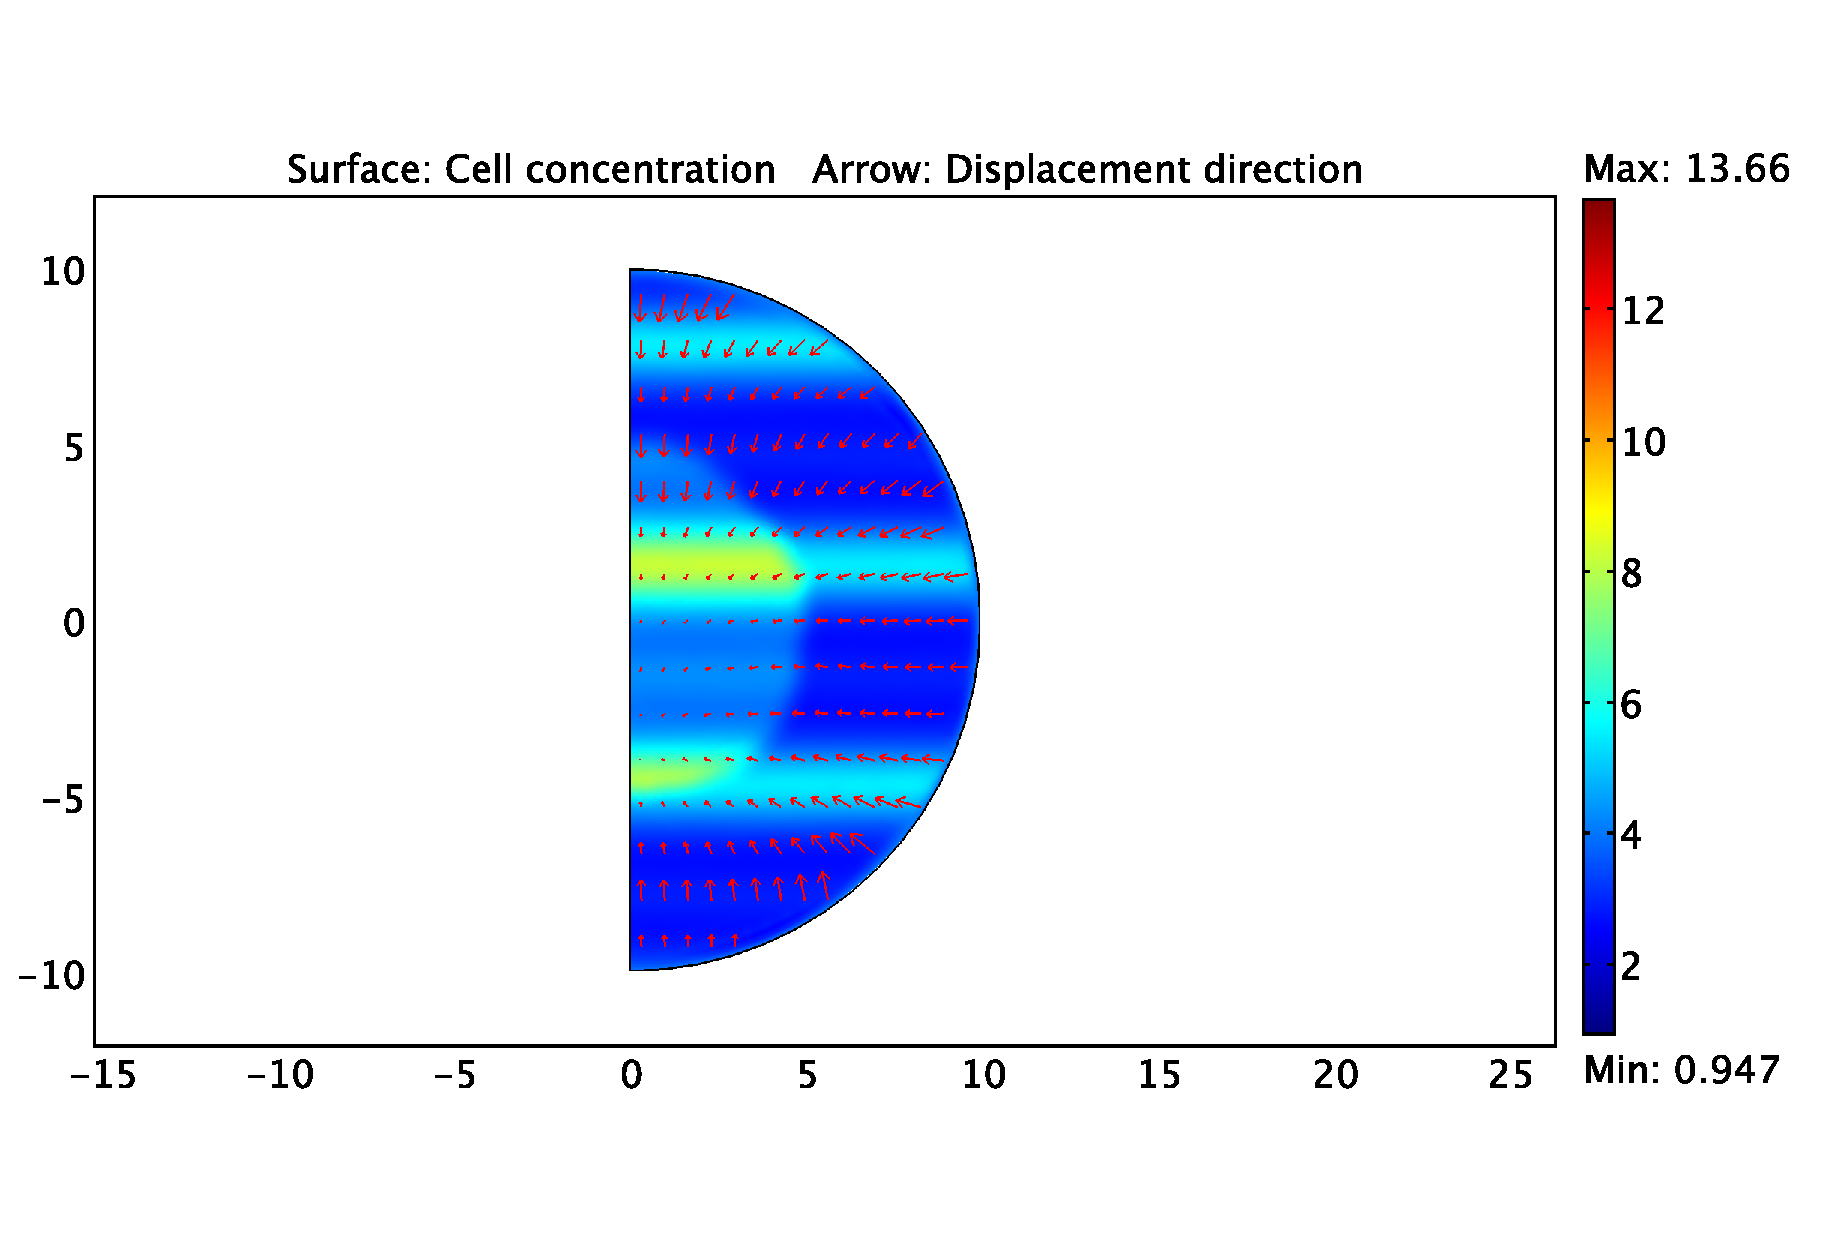
\includegraphics[width=0.9\textwidth]{images/examples/%
eulerian/cancer/haptotaxis-proliferating-cells-3p3}
\caption{Proliferating cells undergoing diffusion and haptotaxis at time $t=33$ days.}
\label{tumour-haptotaxis-proliferation-3p3}
\end{figure}

\begin{figure}[!hptb]
\centering
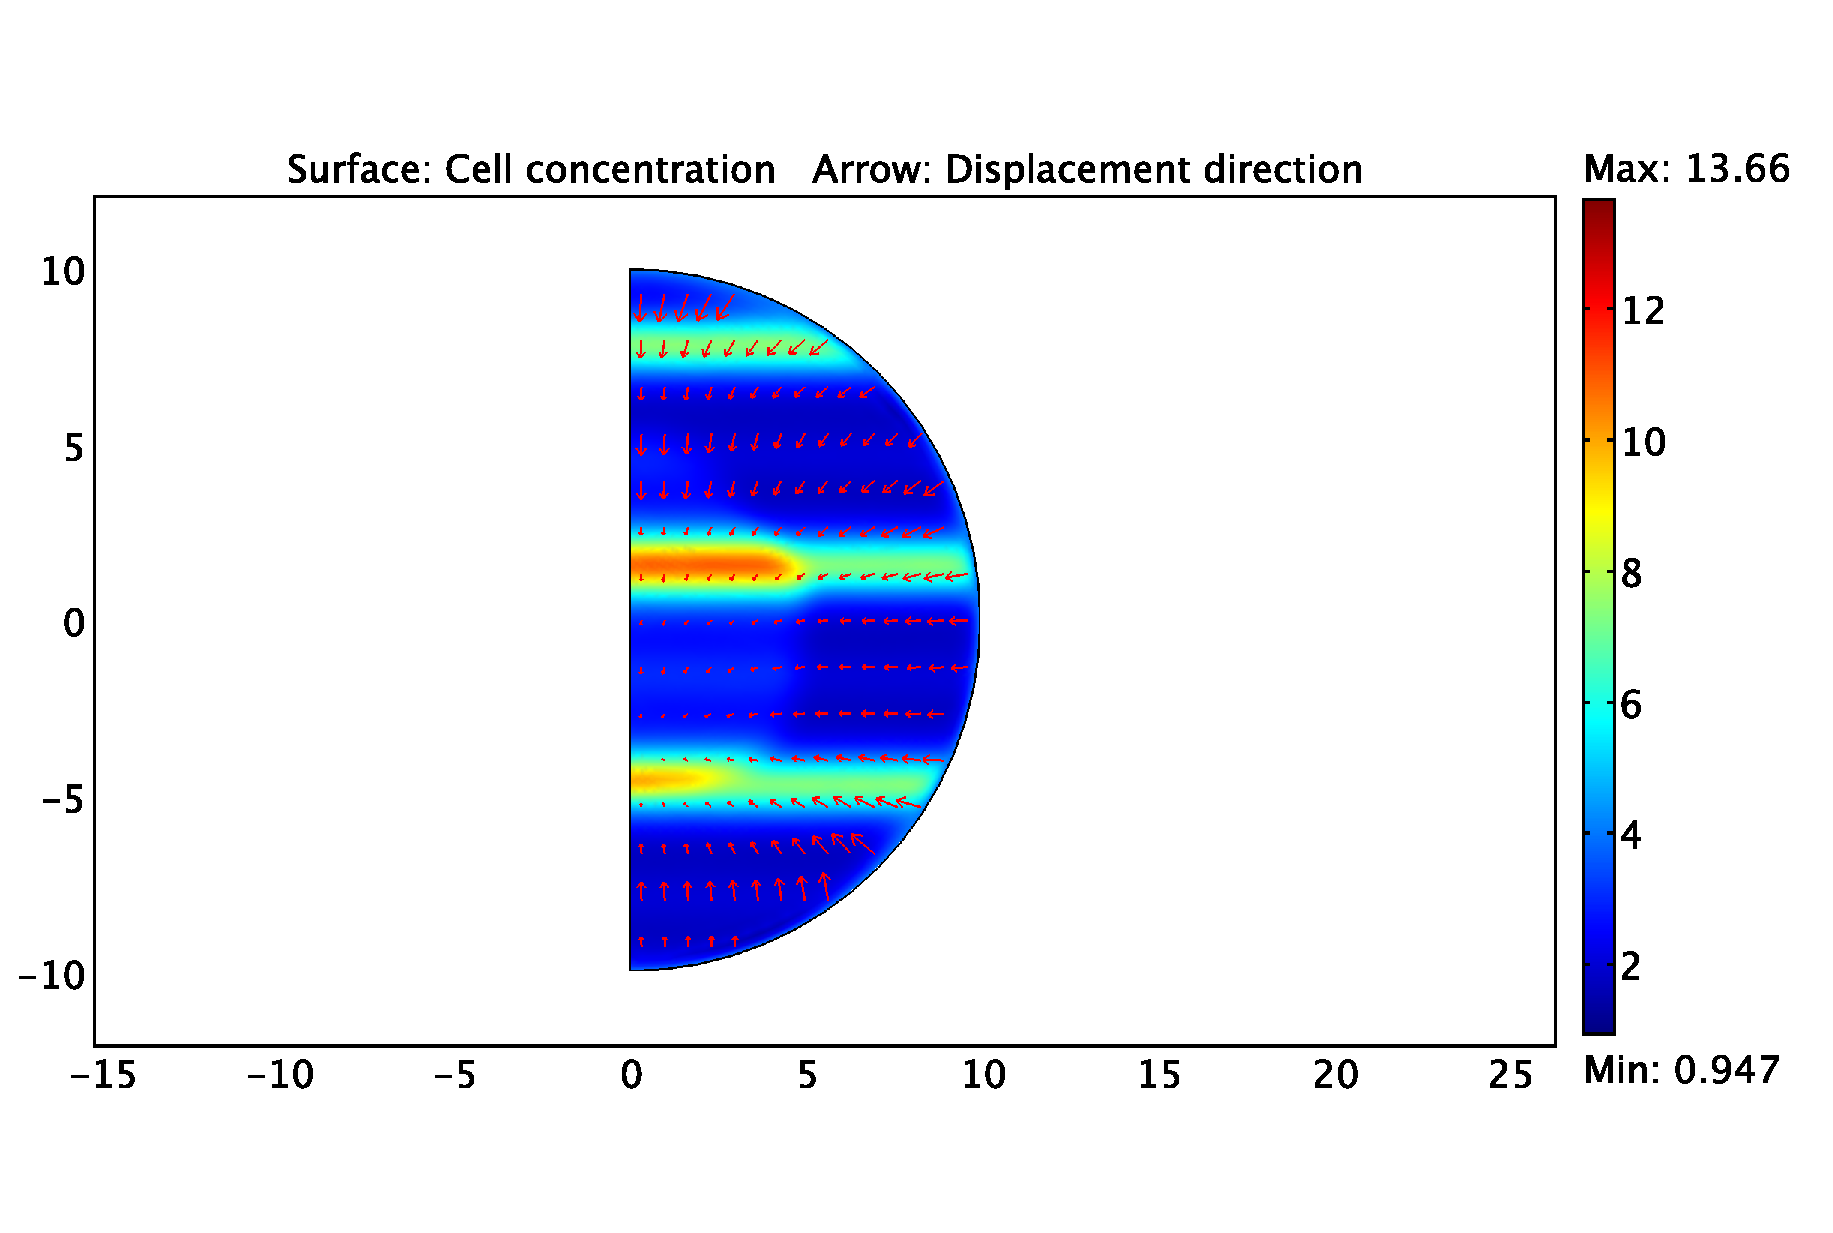
\includegraphics[width=0.9\textwidth]{images/examples/%
eulerian/cancer/haptotaxis-proliferating-cells-6p7}
\caption{Proliferating cells undergoing diffusion and haptotaxis at time $t=67$ days.}
\label{tumour-haptotaxis-proliferation-6p7}
\end{figure}

\begin{figure}[!hptb]
\centering
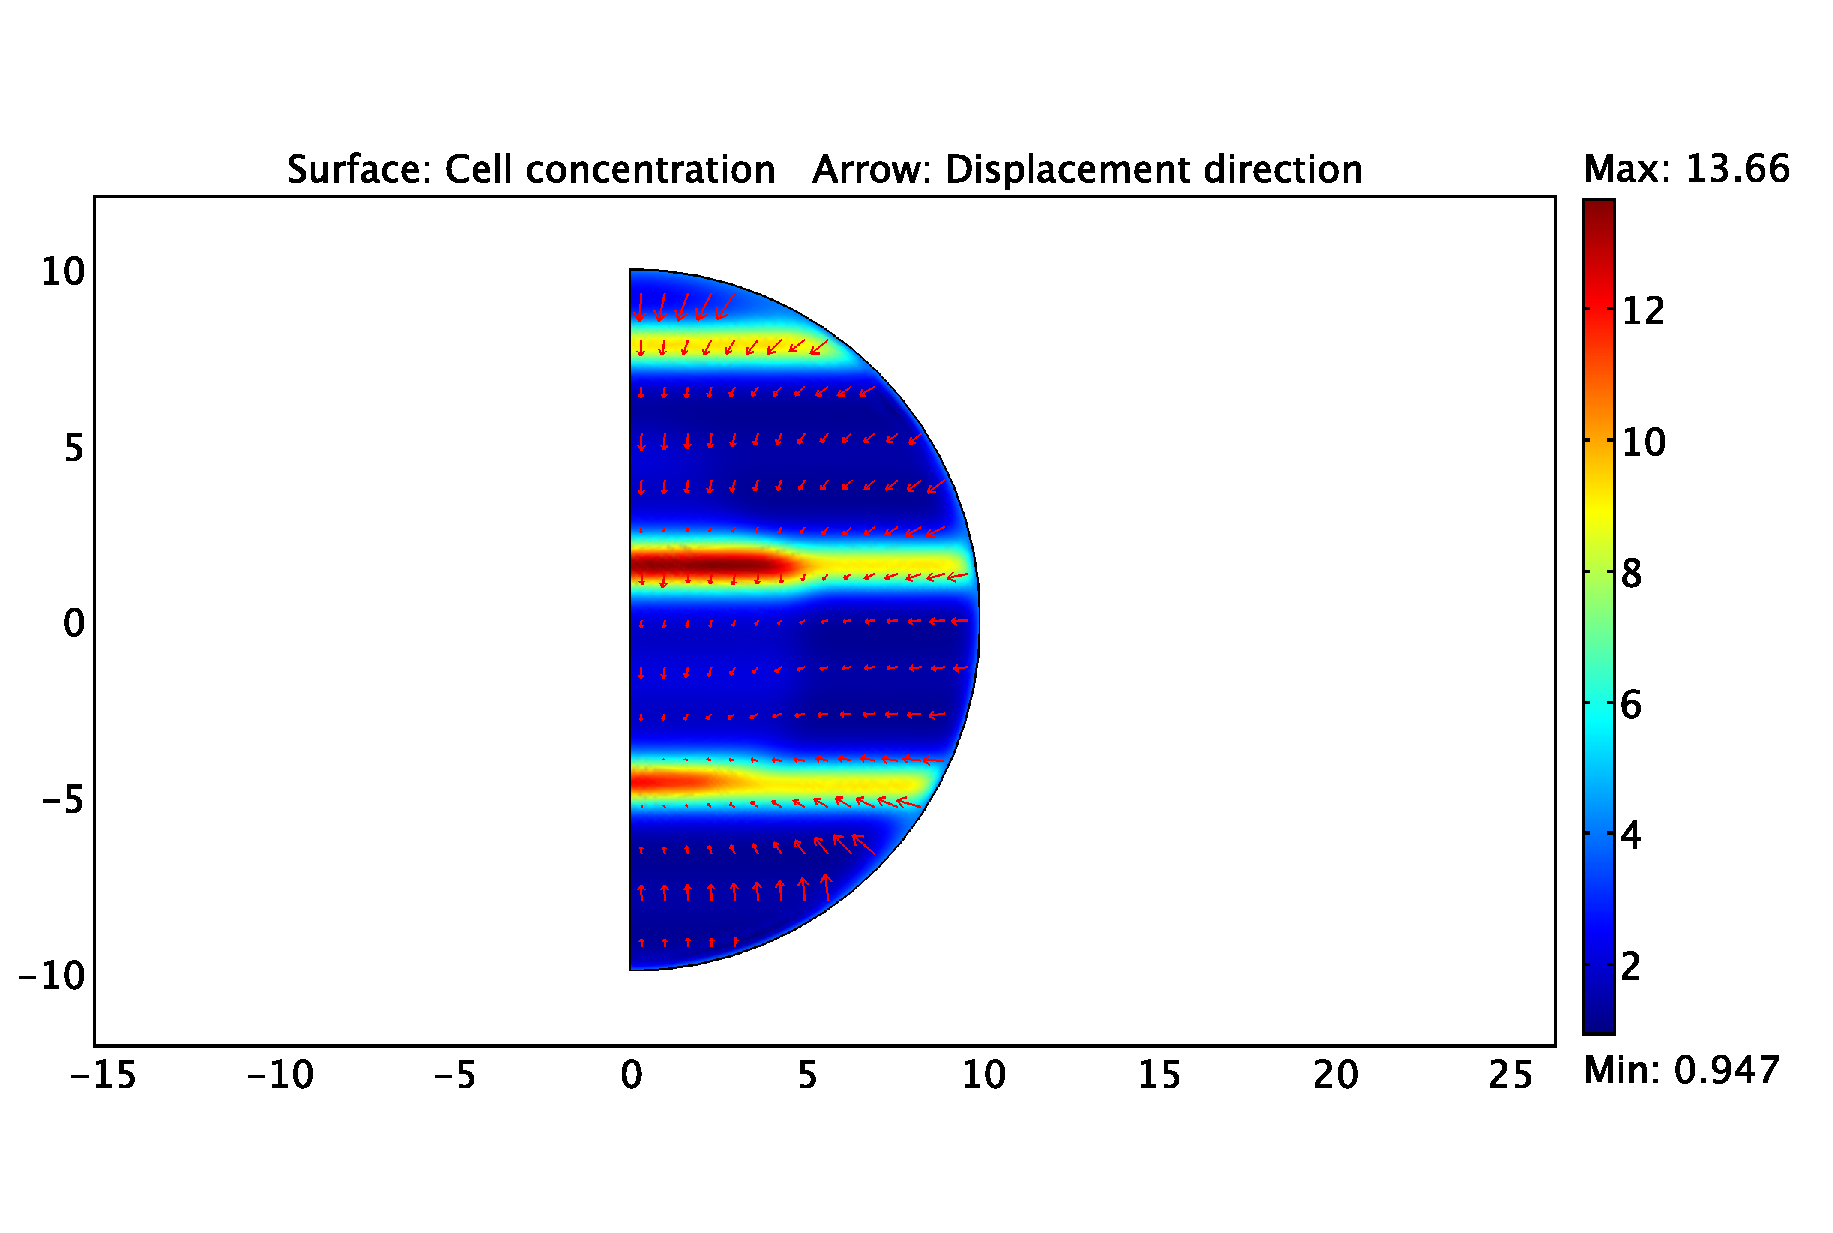
\includegraphics[width=0.9\textwidth]{images/examples/%
eulerian/cancer/haptotaxis-proliferating-cells-10}
\caption{Proliferating cells undergoing diffusion and haptotaxis at time $t=100$ days.}
\label{tumour-haptotaxis-proliferation-10}
\end{figure}

While the magnitudes for the cell diffusivity, $D^{\mathrm{cell}}$,
and haptotactic coefficient, $h$, are arbitrarily chosen, following
the experimental data cited in \citet{namyetal:04}, the value assumed
for $h$ is an order of magnitude greater than that assumed for
$D^{\mathrm{cell}}$, which will ensure that when the two modes for
mass transport are combined, haptotaxis will be the dominant
mechanism.

\subsection{Coupling the phenomena}
\label{cacophonous-medley}

With the individual phenomena explored, we are now ready to solve
the coupled problem described initially. The range of physics
incorporated into this problem include proliferating cells undergoing
both diffusion and haptotaxis, a rate law for the production of
additional ECM which scales linearly with the concentration of
cells, the stress within the cells induced by their traction, the
hyperelastic response of the ECM, isotropic kinematic swelling
associated with the increase in tumour mass, and finally, this
swelling constrained by the presence of the wall.

Figures~\ref{tumour-growth-constrained-0}%
--Figures~\ref{tumour-growth-constrained-5} show snapshots of the
growing tumour constrained by the wall. The colour contours provide
the x-displacement of the swelling tumour and arrows provide the
direction of the velocity field. Observe that the regions that have a
higher cell concentration due to haptotaxis (refer
Figures~\ref{tumour-haptotaxis-proliferation-0}%
--\ref{tumour-haptotaxis-proliferation-10}) tend to swell faster than
regions with lower cell concentrations. Also observe that due to the
presence of the wall, even as early as 2~days, the velocities are
biased toward the vertical direction. Finally, upon comparing these
constrained tumour growth snapshots with
Figure~\ref{tumour-growth-no-wall-4}, which is a result of a similar
calculation without the wall, it is clear that the presence of the
compressive stress along a direction inhibits growth along that
direction, which is what we were aiming to see.

\vspace{1 cm} % Hack

It must be reiterated here that the results provided in this section
are only to demonstrate that varying classes of physics can be
incorporated into the existing mathematical and computational
formulation. These results have been obtained using an isotropic
growth law (\ref{2d-isotropic}), without requiring the
stress-dependent time rate of the growth portion of the deformation
gradient derived in Section~\ref{eu-stress-dependent-growth}. It is
not yet clear whether the constraint from the mechanical loads just
deform the tissue and distort their shape, or whether the cells have
some ability to sense the local stress state and this affects
directionality of further growth. More research into experimental
literature is needed before a conclusive statement can be made.

\vspace{1cm} %Hack

\begin{figure}[!hptb]
\centering
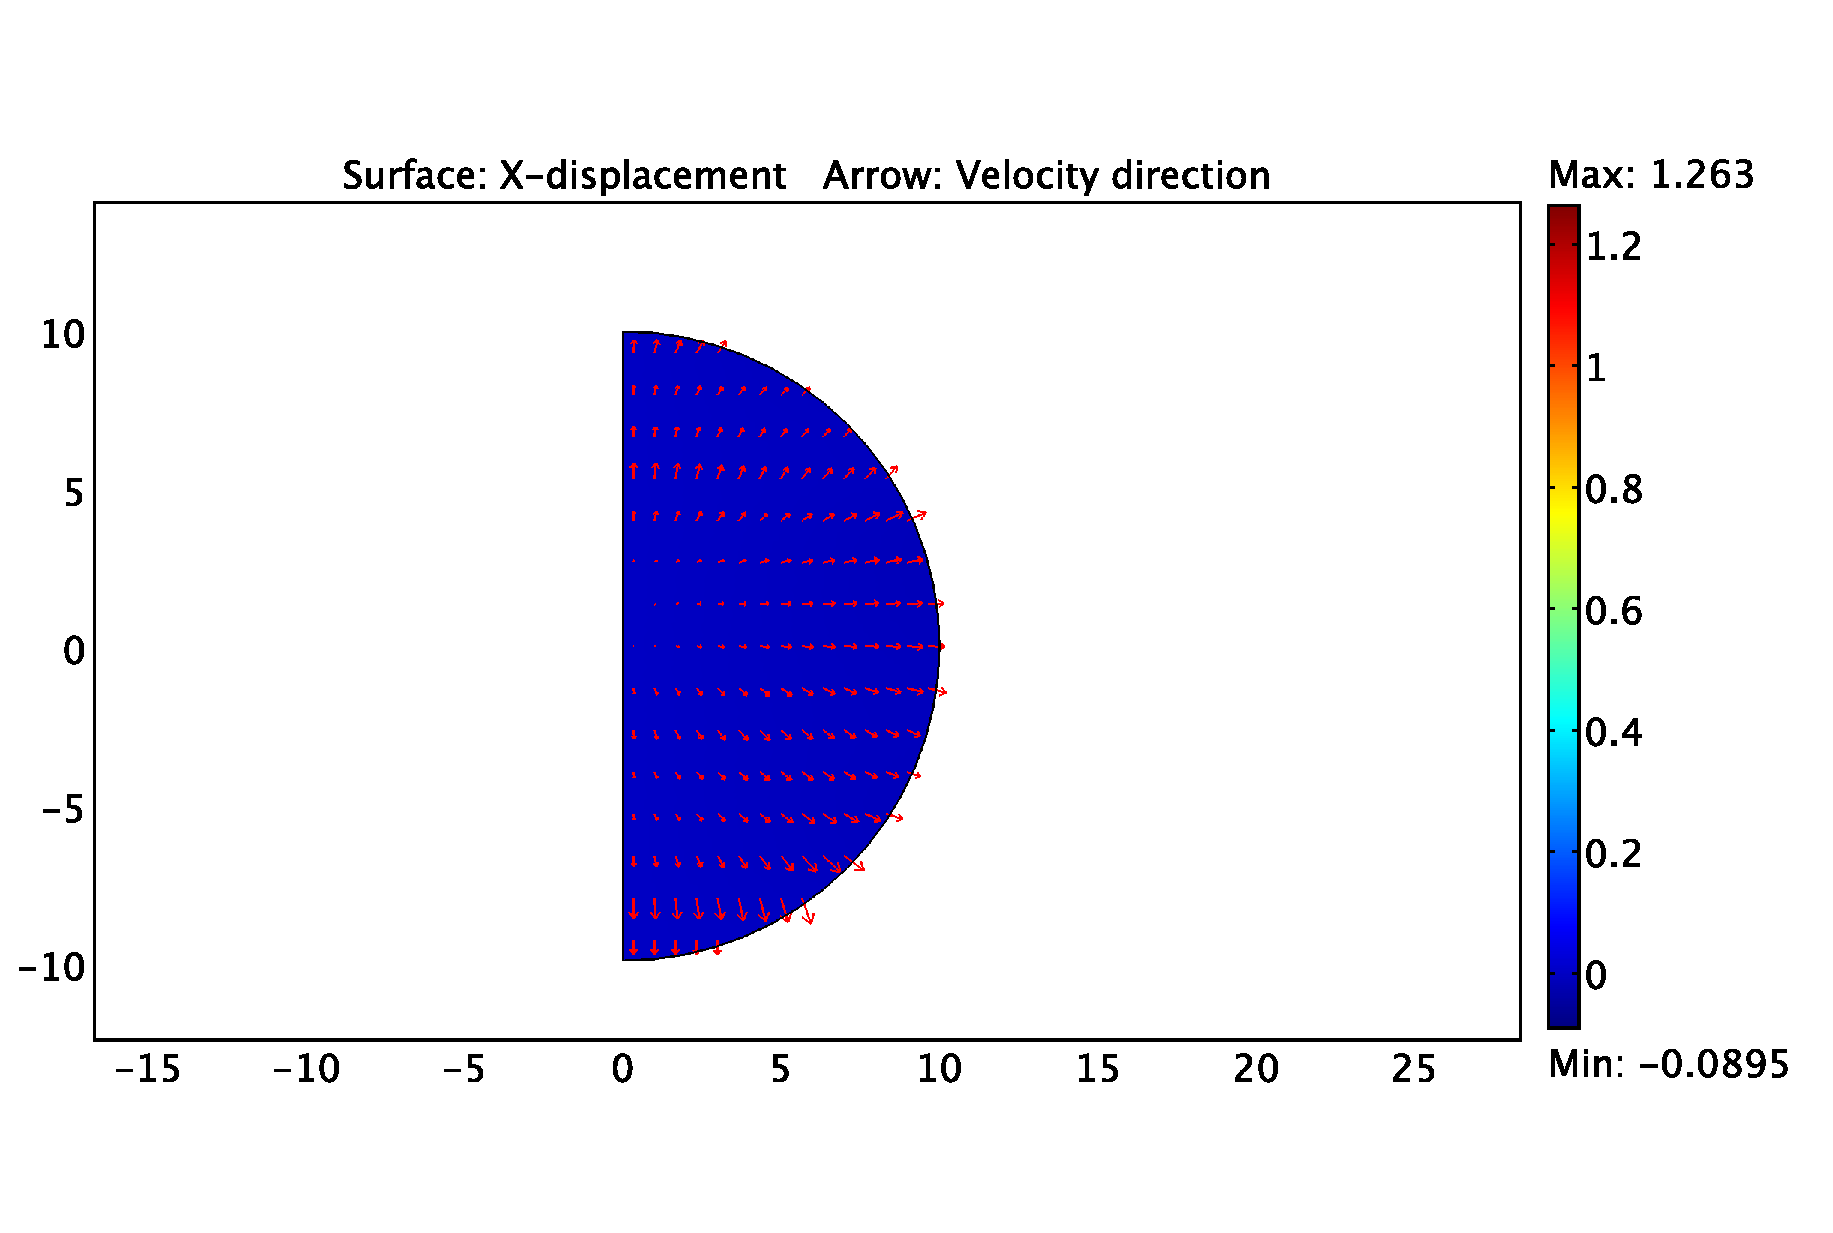
\includegraphics[width=0.9\textwidth]{images/examples/%
eulerian/cancer/growing-tumour-0.eps}
\caption{A constrained growing tumour at $t=0$ days.}
\label{tumour-growth-constrained-0}
\end{figure}

\begin{figure}[!hptb]
\centering
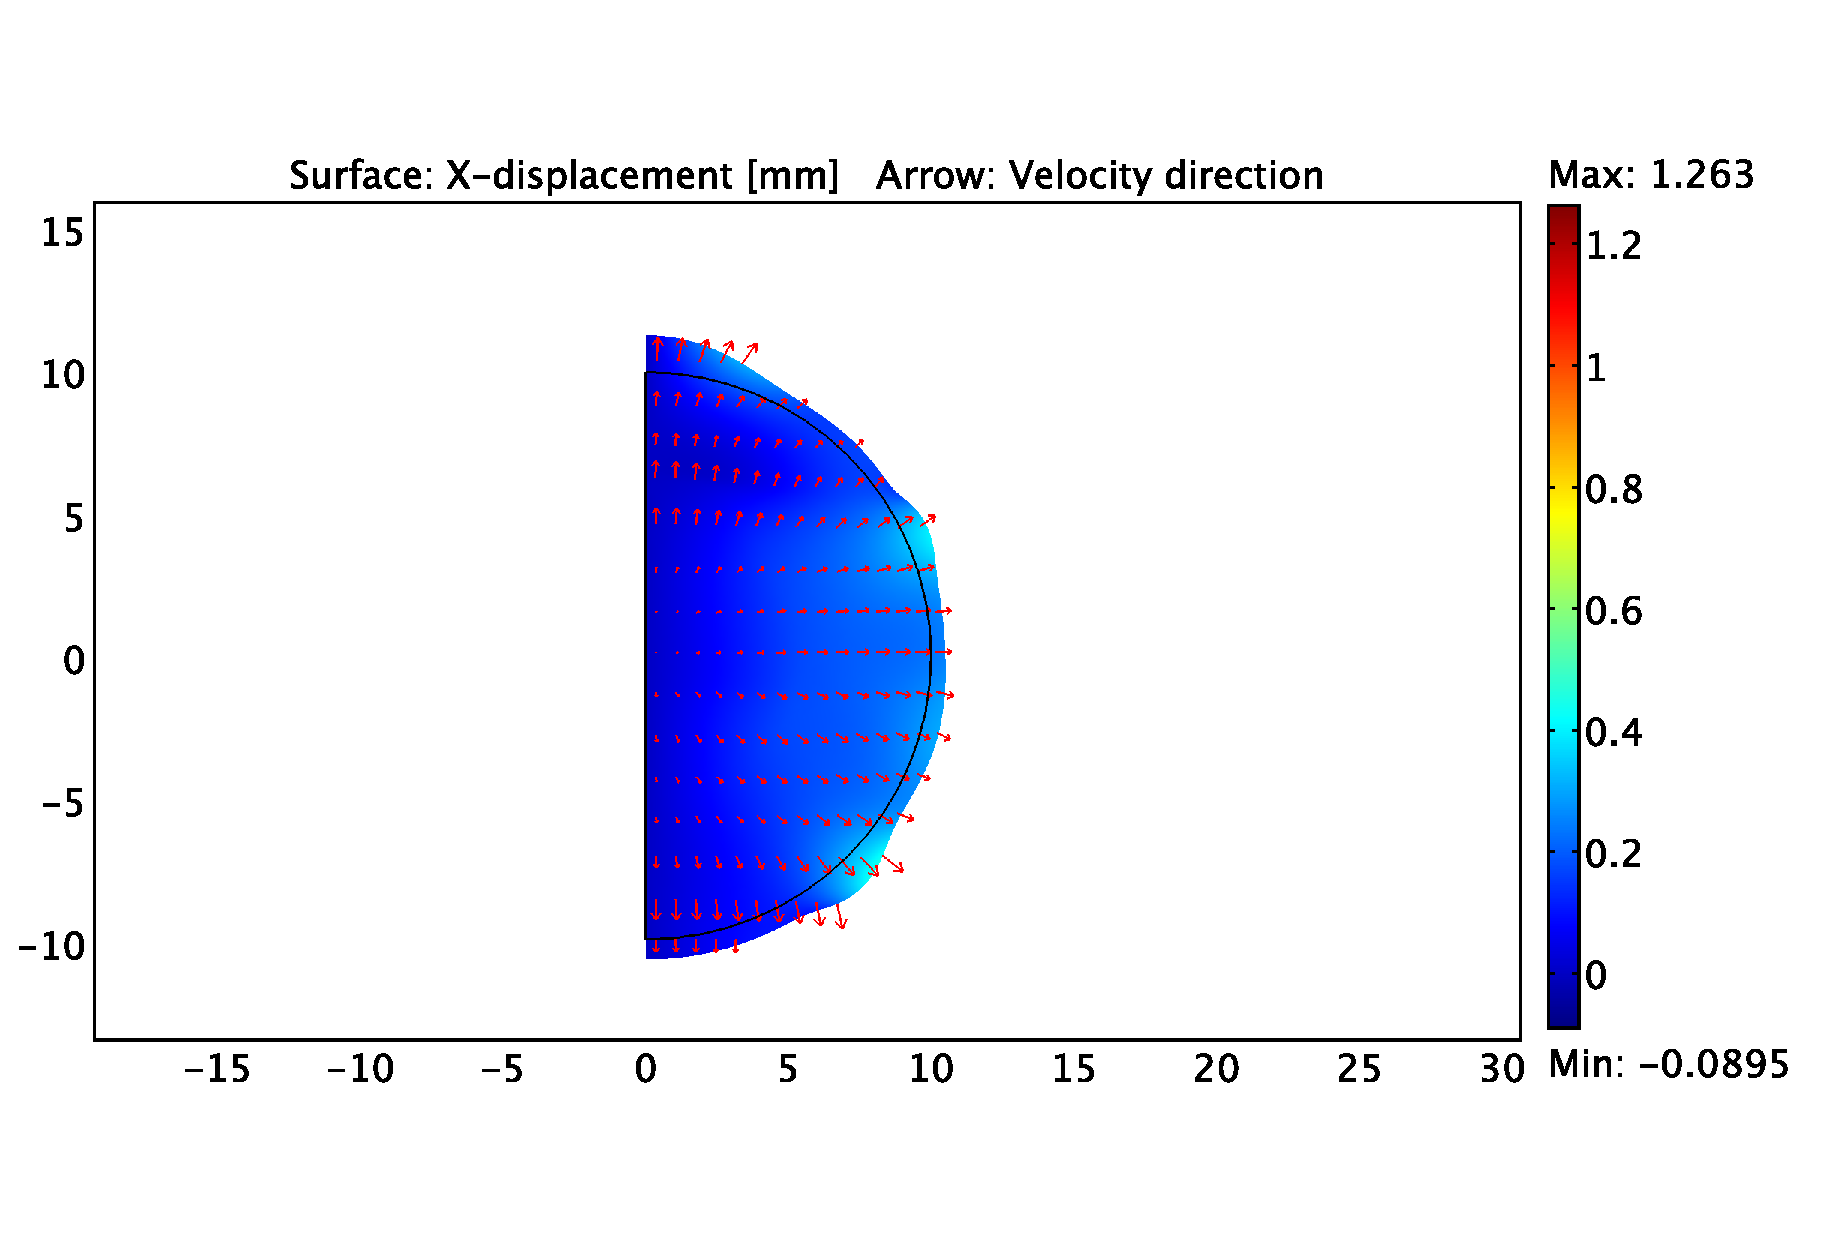
\includegraphics[width=0.9\textwidth]{images/examples/%
eulerian/cancer/growing-tumour-1.eps}
\caption{A constrained growing tumour at $t=20$ days.}
\label{tumour-growth-constrained-1}
\end{figure}

\begin{figure}[!hptb]
\centering
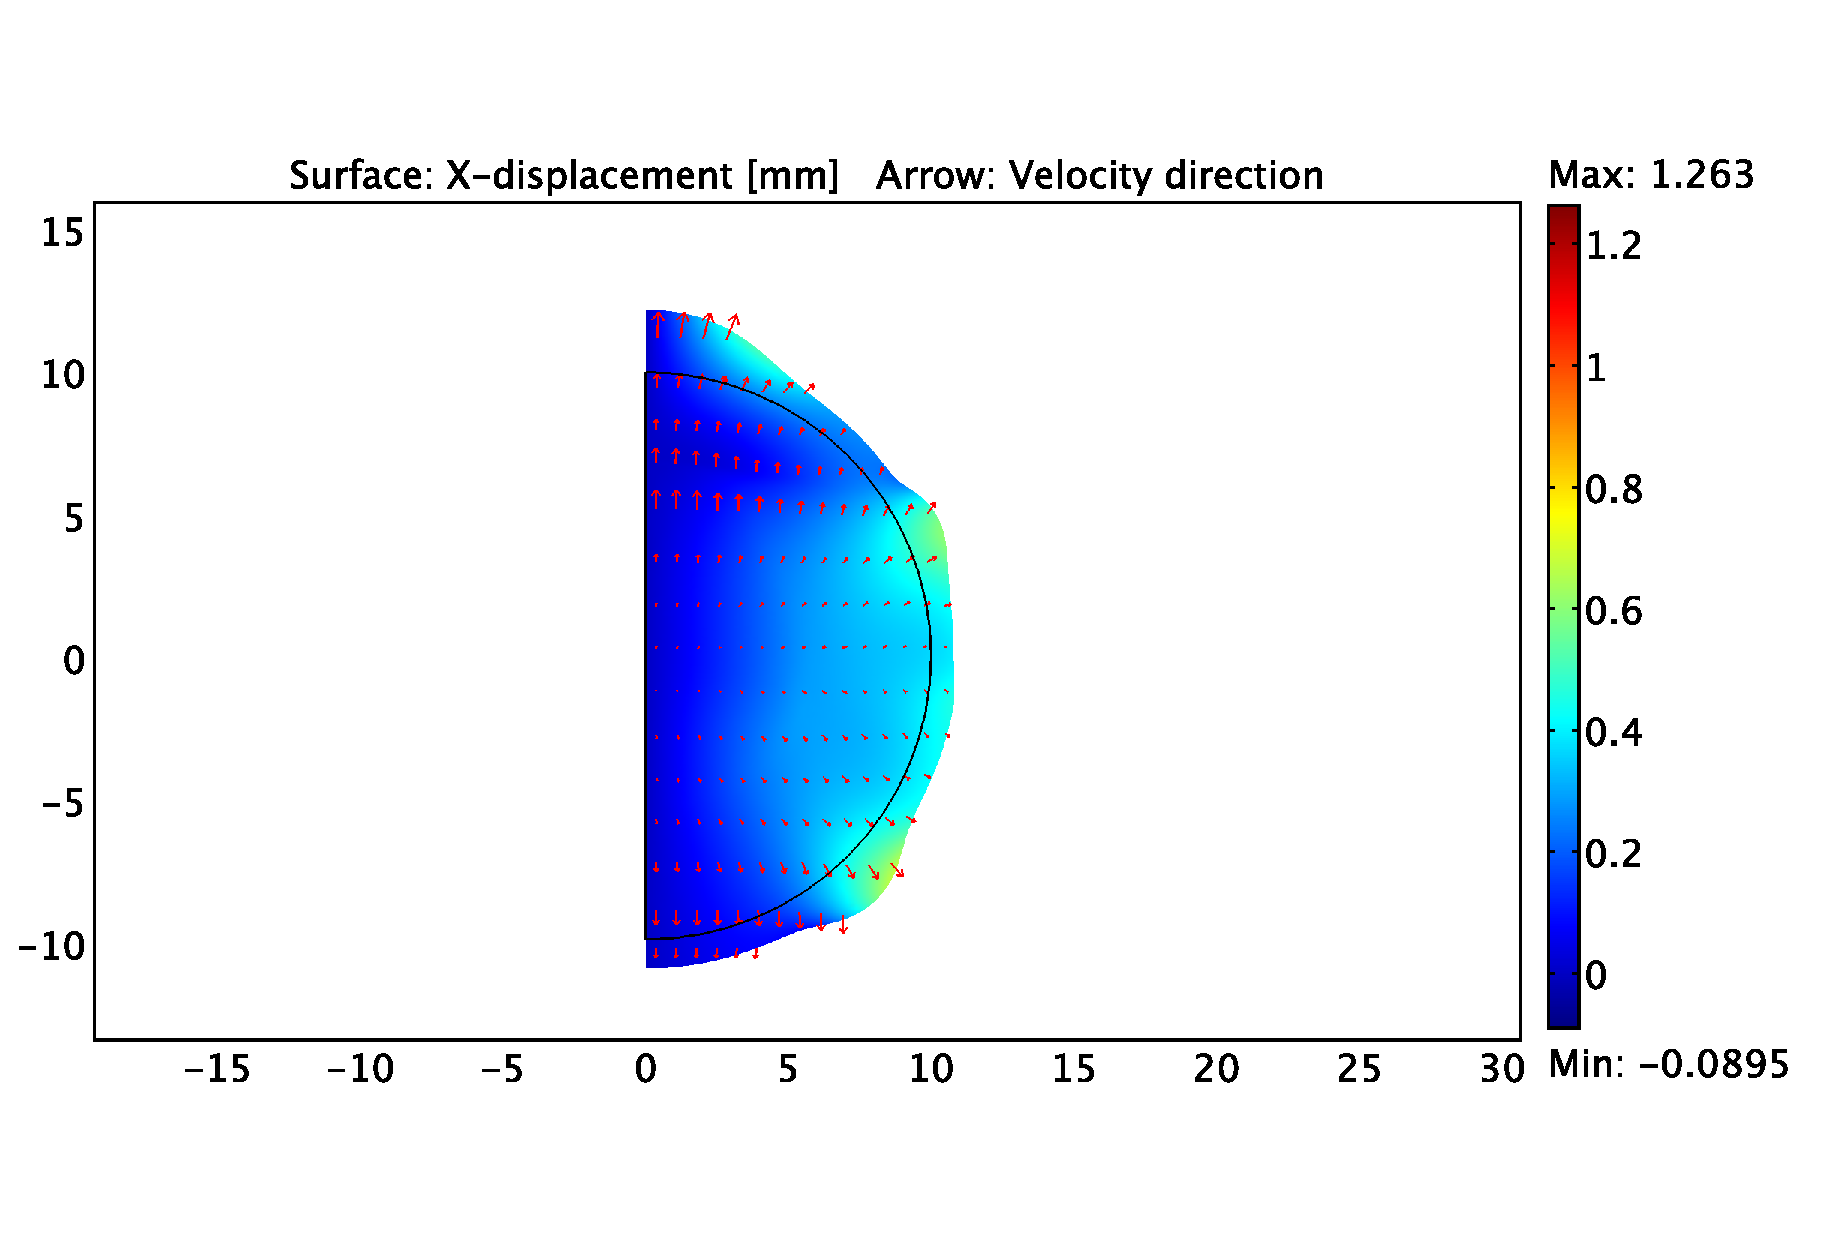
\includegraphics[width=0.9\textwidth]{images/examples/%
eulerian/cancer/growing-tumour-2.eps}
\caption{A constrained growing tumour at $t=40$ days.}
\label{tumour-growth-constrained-2}
\end{figure}

\begin{figure}[!hptb]
\centering
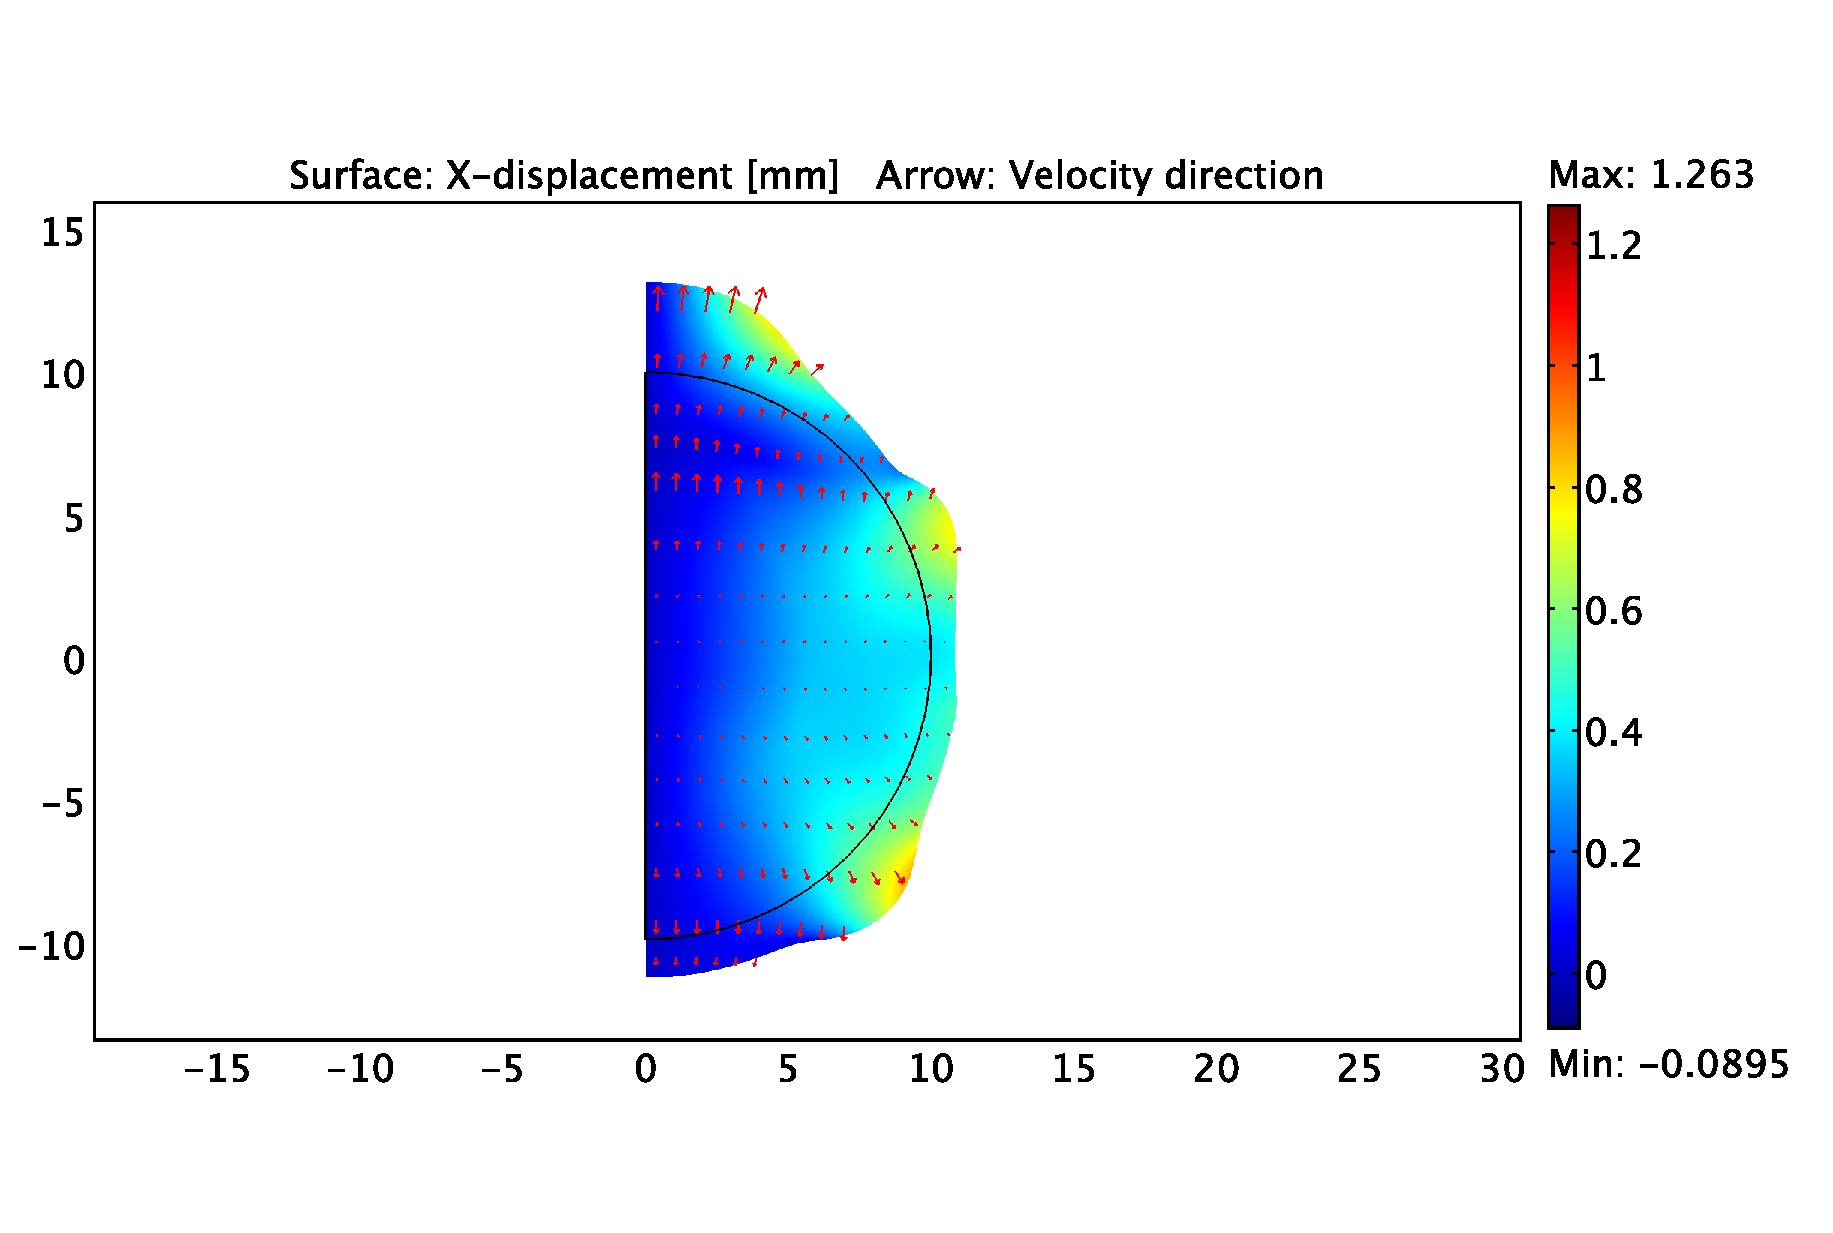
\includegraphics[width=0.9\textwidth]{images/examples/%
eulerian/cancer/growing-tumour-3.eps}
\caption{A constrained growing tumour at $t=60$ days.}
\label{tumour-growth-constrained-3}
\end{figure}

\begin{figure}[!hptb]
\centering
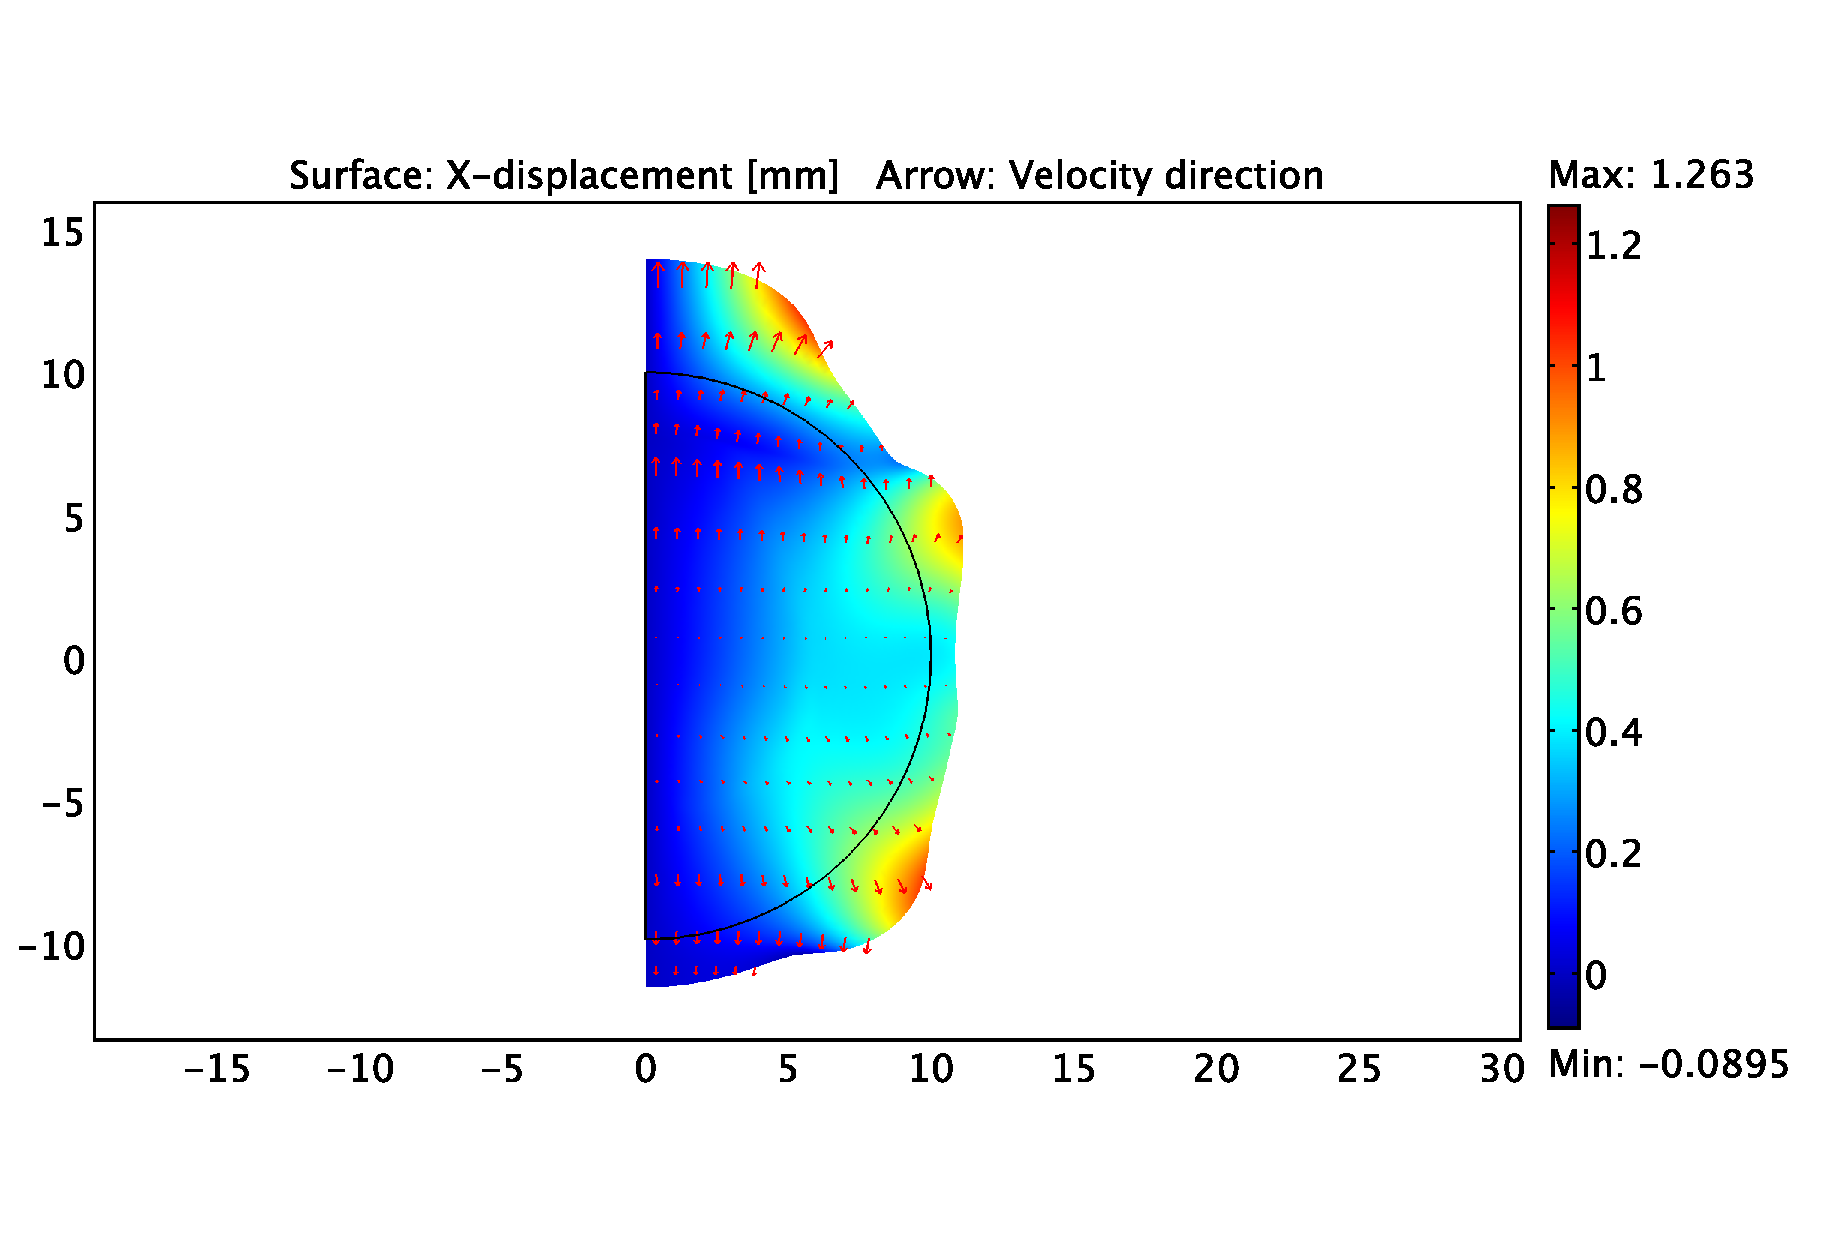
\includegraphics[width=0.9\textwidth]{images/examples/%
eulerian/cancer/growing-tumour-4.eps}
\caption{A constrained growing tumour at $t=80$ days.}
\label{tumour-growth-constrained-4}
\end{figure}

\begin{figure}[!hptb]
\centering
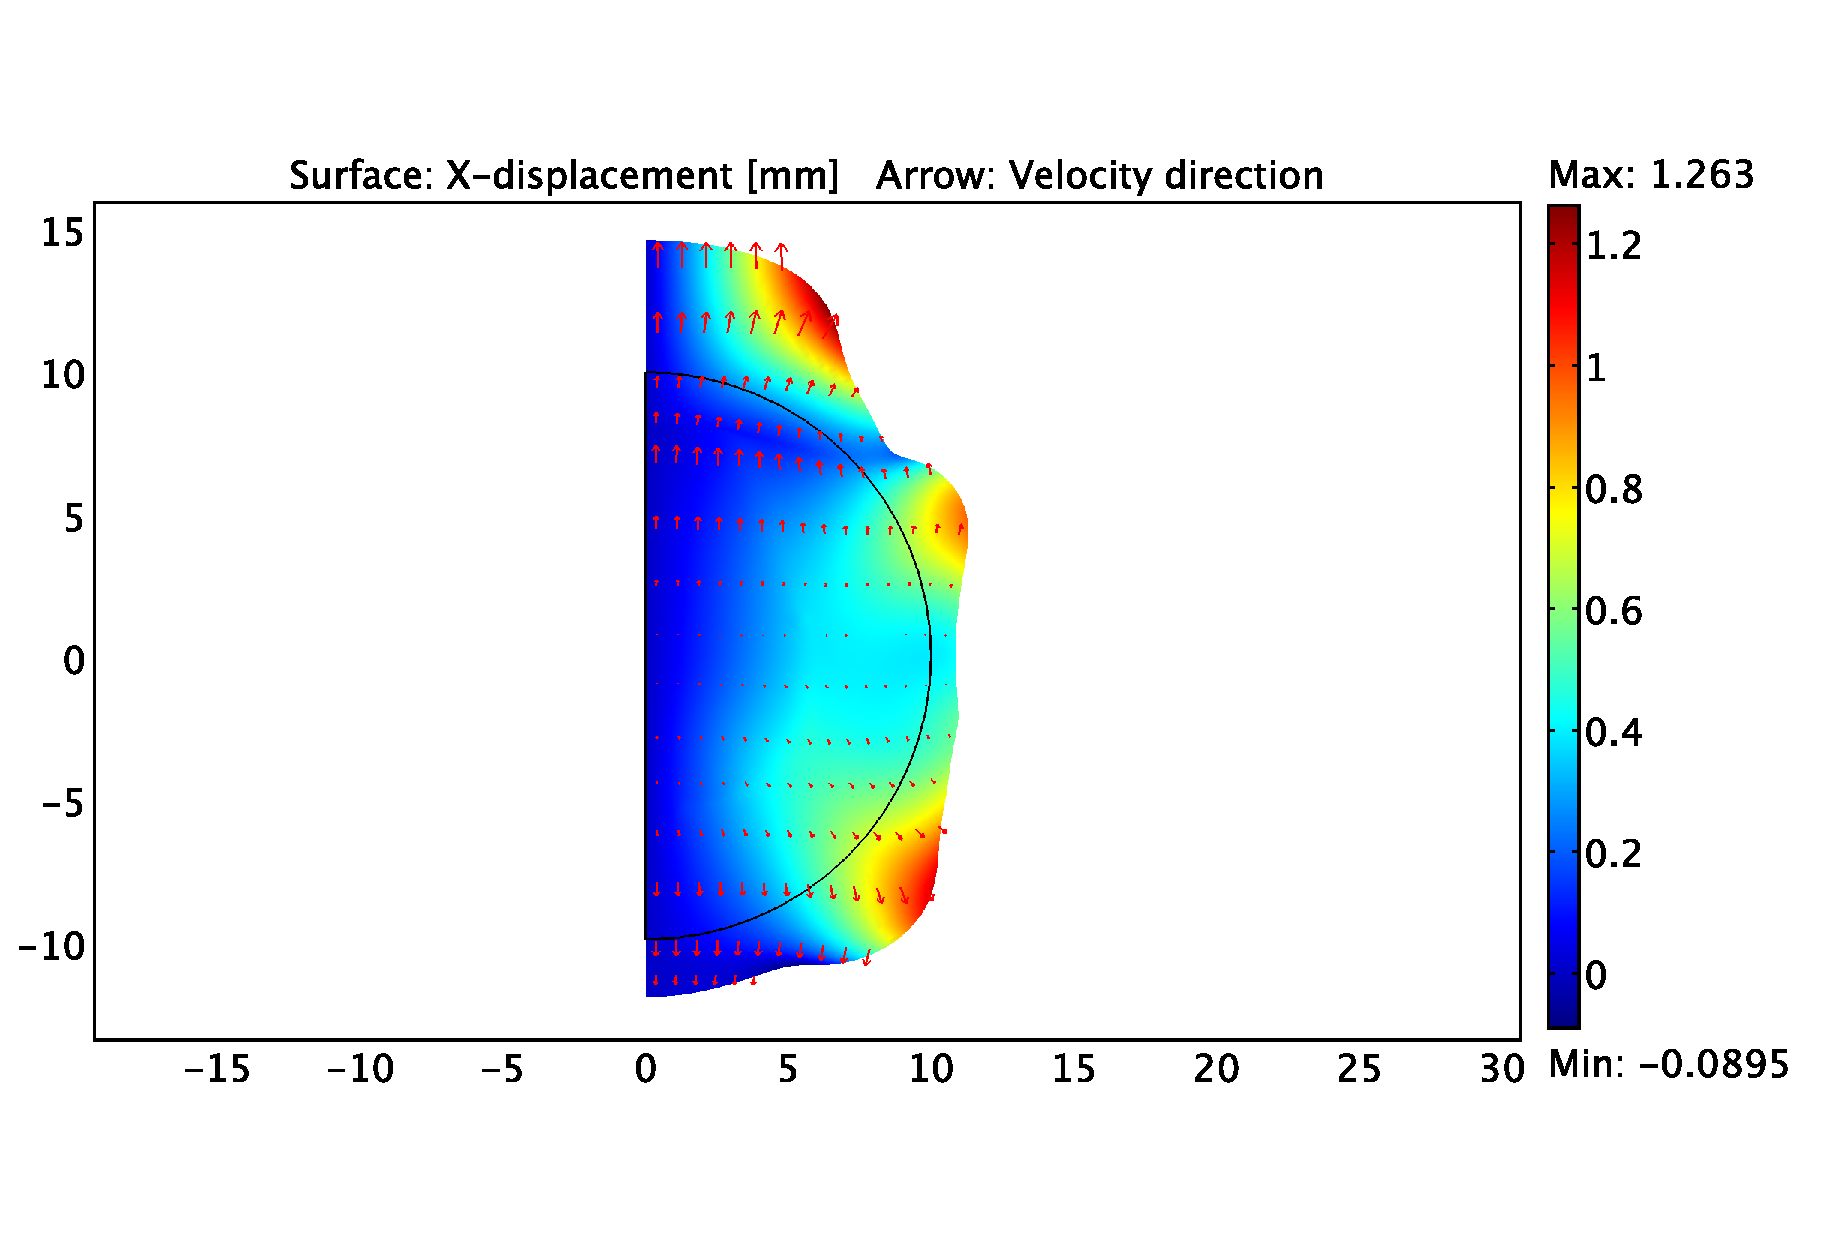
\includegraphics[width=0.9\textwidth]{images/examples/%
eulerian/cancer/growing-tumour-5.eps}
\caption{A constrained growing tumour at $t=100$ days.}
\label{tumour-growth-constrained-5}
\end{figure}

\begin{figure}[!hptb]
\centering
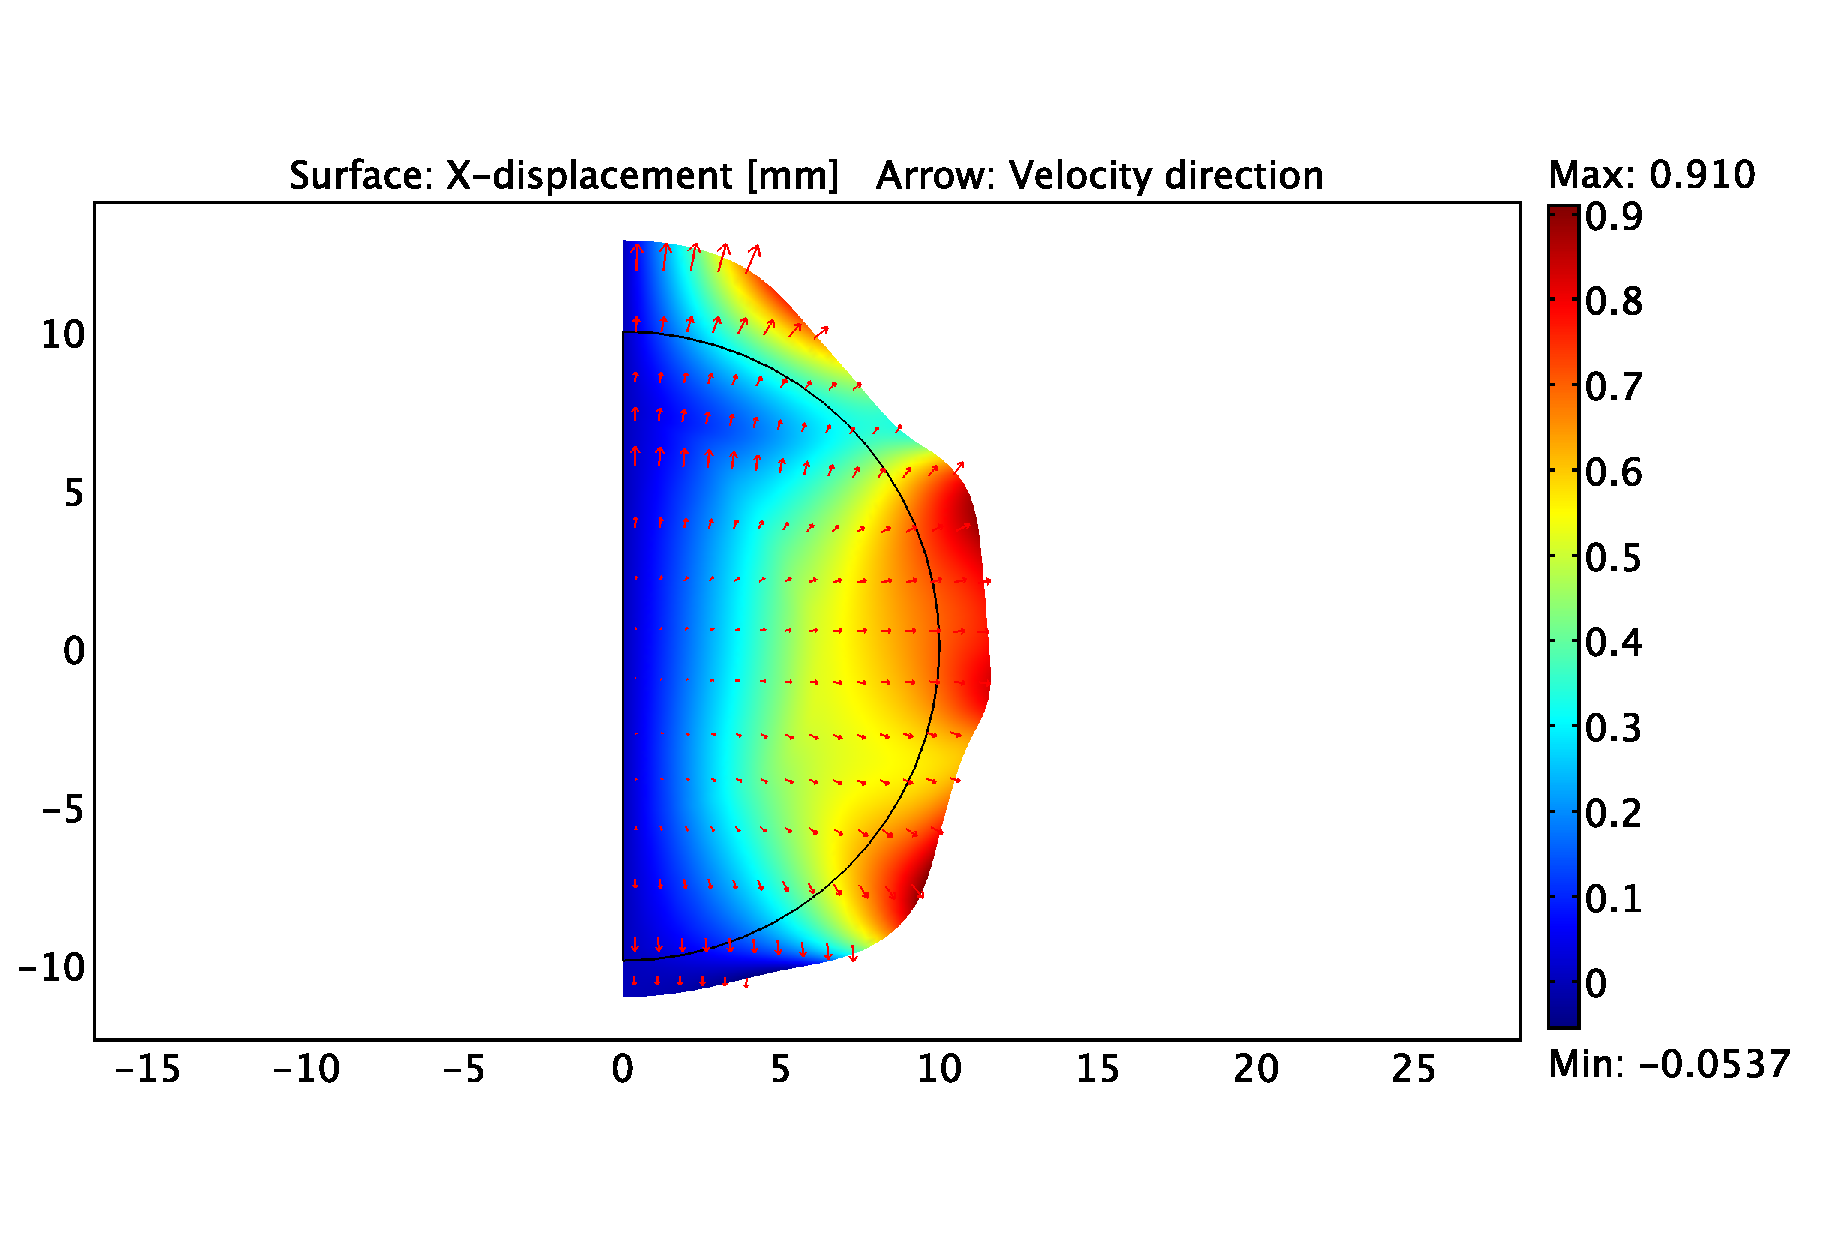
\includegraphics[width=0.9\textwidth]{images/examples/%
eulerian/cancer/growing-tumour-no-wall-4}
\caption{An unconstrained growing tumour at $t=80$ days.}
\label{tumour-growth-no-wall-4}
\end{figure}

%

% Local Variables:
% TeX-master: "thesis"
% mode: latex
% mode: flyspell
% End:
